%==============================================================================
% Tento soubor použijte jako základ
% This file should be used as a base for the thesis
% Autoři / Authors: 2008 Michal Bidlo, 2022 Jaroslav Dytrych
% Kontakt pro dotazy a připomínky: sablona@fit.vutbr.cz
% Contact for questions and comments: sablona@fit.vutbr.cz
%==============================================================================
% kódování: UTF-8 (zmena prikazem iconv, recode nebo cstocs)
% encoding: UTF-8 (you can change it by command iconv, recode or cstocs)
%------------------------------------------------------------------------------
% zpracování / processing: make, make pdf, make clean
%==============================================================================
% Soubory, které je nutné upravit nebo smazat: / Files which have to be edited or deleted:
%   xmiska03-Zobrazeni_dat_z_zeleznicniho_MMS-20-literatura-bibliography.bib - literatura / bibliography
%   xmiska03-Zobrazeni_dat_z_zeleznicniho_MMS-01-kapitoly-chapters.tex - obsah práce / the thesis content
%   xmiska03-Zobrazeni_dat_z_zeleznicniho_MMS-01-kapitoly-chapters-en.tex - obsah práce v angličtině / the thesis content in English
%   xmiska03-Zobrazeni_dat_z_zeleznicniho_MMS-30-prilohy-appendices.tex - přílohy / appendices
%   xmiska03-Zobrazeni_dat_z_zeleznicniho_MMS-30-prilohy-appendices-en.tex - přílohy v angličtině / appendices in English
%==============================================================================
\documentclass[slovak, zadani]{fitthesis} % bez zadání - pro začátek práce, aby nebyl problém s překladem
%\documentclass[english]{fitthesis} % without assignment - for the work start to avoid compilation problem
%\documentclass[zadani]{fitthesis} % odevzdani do IS VUT a/nebo tisk s barevnými odkazy - odkazy jsou barevné
%\documentclass[english,zadani]{fitthesis} % for submission to the IS VUT and/or print with color links - links are color
%\documentclass[zadani,print]{fitthesis} % pro černobílý tisk - odkazy jsou černé
%\documentclass[english,zadani,print]{fitthesis} % for the black and white print - links are black
%\documentclass[zadani,cprint]{fitthesis} % pro barevný tisk - odkazy jsou černé, znak VUT barevný
%\documentclass[english,zadani,cprint]{fitthesis} % for the print - links are black, logo is color
% * Je-li práce psaná v anglickém jazyce, je zapotřebí u třídy použít 
%   parametr english následovně:
%   If thesis is written in English, it is necessary to use 
%   parameter english as follows:
%      \documentclass[english]{fitthesis}
% * Je-li práce psaná ve slovenském jazyce, je zapotřebí u třídy použít 
%   parametr slovak následovně:
%   If the work is written in the Slovak language, it is necessary 
%   to use parameter slovak as follows:
%      \documentclass[slovak]{fitthesis}
% * Je-li práce psaná v anglickém jazyce se slovenským abstraktem apod., 
%   je zapotřebí u třídy použít parametry english a enslovak následovně:
%   If the work is written in English with the Slovak abstract, etc., 
%   it is necessary to use parameters english and enslovak as follows:
%      \documentclass[english,enslovak]{fitthesis}

% Základní balíčky jsou dole v souboru šablony fitthesis.cls
% Basic packages are at the bottom of template file fitthesis.cls
% zde můžeme vložit vlastní balíčky / you can place own packages here


% Pro seznam zkratek lze využít balíček Glossaries - nutno odkomentovat i níže a při kompilaci z konzoly i v Makefile (plnou verzi pro Perl, nebo lite)
% The Glossaries package can be used for the list of abbreviations - it is necessary to uncomment also below. When compiling from the console also in the Makefile (full version for Perl or lite)
%\usepackage{glossaries}
%\usepackage{glossary-superragged}
%\makeglossaries 

% Nastavení cesty k obrázkům
% Setting of a path to the pictures
%\graphicspath{{obrazky-figures/}{./obrazky-figures/}}
%\graphicspath{{obrazky-figures/}{../obrazky-figures/}}

%---rm---------------
\renewcommand{\rmdefault}{lmr}%zavede Latin Modern Roman jako rm / set Latin Modern Roman as rm
%---sf---------------
\renewcommand{\sfdefault}{qhv}%zavede TeX Gyre Heros jako sf
%---tt------------
\renewcommand{\ttdefault}{lmtt}% zavede Latin Modern tt jako tt

% vypne funkci šablony, která automaticky nahrazuje uvozovky,
% aby nebyly prováděny nevhodné náhrady v popisech API apod.
% disables function of the template which replaces quotation marks
% to avoid unnecessary replacements in the API descriptions etc.
\csdoublequotesoff

\usepackage{url}

% =======================================================================
% balíček "hyperref" vytváří klikací odkazy v pdf, pokud tedy použijeme pdflatex
% problém je, že balíček hyperref musí být uveden jako poslední, takže nemůže
% být v šabloně
% "hyperref" package create clickable links in pdf if you are using pdflatex.
% Problem is that this package have to be introduced as the last one so it 
% can not be placed in the template file.
\ifWis
\ifx\pdfoutput\undefined % nejedeme pod pdflatexem / we are not using pdflatex
\else
  \usepackage{color}
  \usepackage[unicode,colorlinks,hyperindex,plainpages=false,pdftex]{hyperref}
  \definecolor{hrcolor-ref}{RGB}{223,52,30}
  \definecolor{hrcolor-cite}{HTML}{2F8F00}
  \definecolor{hrcolor-urls}{HTML}{092EAB}
  \hypersetup{
	linkcolor=hrcolor-ref,
	citecolor=hrcolor-cite,
	filecolor=magenta,
	urlcolor=hrcolor-urls
  }
  \def\pdfBorderAttrs{/Border [0 0 0] }  % bez okrajů kolem odkazů / without margins around links
  \pdfcompresslevel=9
\fi
\else % pro tisk budou odkazy, na které se dá klikat, černé / for the print clickable links will be black
\ifx\pdfoutput\undefined % nejedeme pod pdflatexem / we are not using pdflatex
\else
  \usepackage{color}
  \usepackage[unicode,colorlinks,hyperindex,plainpages=false,pdftex,urlcolor=black,linkcolor=black,citecolor=black]{hyperref}
  \definecolor{links}{rgb}{0,0,0}
  \definecolor{anchors}{rgb}{0,0,0}
  \def\AnchorColor{anchors}
  \def\LinkColor{links}
  \def\pdfBorderAttrs{/Border [0 0 0] } % bez okrajů kolem odkazů / without margins around links
  \pdfcompresslevel=9
\fi
\fi
% Řešení problému, kdy klikací odkazy na obrázky vedou za obrázek
% This solves the problems with links which leads after the picture
\usepackage[all]{hypcap}
\usepackage{listings}

% Informace o práci/projektu / Information about the thesis
%---------------------------------------------------------------------------
\projectinfo{
  %Prace / Thesis
  project={BP},            %typ práce BP/SP/DP/DR  / thesis type (SP = term project)
  year={2025},             % rok odevzdání / year of submission
  date=\today,             % datum odevzdání / submission date
  %Nazev prace / thesis title
  title.cs={Zobrazení lidarových, kamerových a~vektorových dat z~železničního mobilního mapovacího systému},  % název práce v češtině či slovenštině (dle zadání) / thesis title in czech language (according to assignment)
  title.en={Thesis title}, % název práce v angličtině / thesis title in english
  title.length={12.8cm}, % nastavení délky bloku s titulkem pro úpravu zalomení řádku (lze definovat zde nebo níže) / setting the length of a block with a thesis title for adjusting a line break (can be defined here or below)
  %sectitle.length={14.5cm}, % nastavení délky bloku s druhým titulkem pro úpravu zalomení řádku (lze definovat zde nebo níže) / setting the length of a block with a second thesis title for adjusting a line break (can be defined here or below)
  %dectitle.length={14.5cm}, % nastavení délky bloku s titulkem nad prohlášením pro úpravu zalomení řádku (lze definovat zde nebo níže) / setting the length of a block with a thesis title above declaration for adjusting a line break (can be defined here or below)
  %Autor / Author
  author.name={Zuzana},   % jméno autora / author name
  author.surname={Miškaňová},   % příjmení autora / author surname 
  %author.title.p={Bc.}, % titul před jménem (nepovinné) / title before the name (optional)
  %author.title.a={Ph.D.}, % titul za jménem (nepovinné) / title after the name (optional)
  %Ustav / Department
  department={UPGM}, % doplňte příslušnou zkratku dle ústavu na zadání: UPSY/UIFS/UITS/UPGM / fill in appropriate abbreviation of the department according to assignment: UPSY/UIFS/UITS/UPGM
  % Školitel / supervisor
  supervisor.name={Ondřej},   % jméno školitele / supervisor name 
  supervisor.surname={Klíma},   % příjmení školitele / supervisor surname
  supervisor.title.p={Ing.},   %titul před jménem (nepovinné) / title before the name (optional)
  supervisor.title.a={Ph.D.},    %titul za jménem (nepovinné) / title after the name (optional)
  % Klíčová slova / keywords
  keywords.cs={vizualizácia dát, dierkový model kamery, mračno bodov, Python, deck.gl, webové aplikácie, Dash}, % klíčová slova v českém či slovenském jazyce / keywords in czech or slovak language
  keywords.en={data visualization, pinhole camera model, point cloud, Python, deck.gl, web aplications, Dash}, % klíčová slova v anglickém jazyce / keywords in english
  %keywords.en={Here, individual keywords separated by commas will be written in English.},
  % Abstrakt / Abstract
  abstract.cs={Do tohoto odstavce bude zapsán výtah (abstrakt) práce v českém (slovenském) jazyce.}, % abstrakt v českém či slovenském jazyce / abstract in czech or slovak language
  abstract.en={Do tohoto odstavce bude zapsán výtah (abstrakt) práce v anglickém jazyce.}, % abstrakt v anglickém jazyce / abstract in english
  %abstract.en={An abstract of the work in English will be written in this paragraph.},
  % Prohlášení (u anglicky psané práce anglicky, u slovensky psané práce slovensky; u projektové praxe lze zakomentovat) / Declaration (for thesis in english should be in english; for project practice can be commented out)
  declaration={ Prehlasujem... %Prohlašuji, že jsem tuto bakalářskou práci vypracoval samostatně pod vedením pana X...
%Další informace mi poskytli...
%Uvedl jsem všechny literární prameny, publikace a další zdroje, ze kterých jsem čerpal.
},
  %declaration={I hereby declare that this Bachelor's thesis was prepared as an original work by the author under the supervision of Mr. X
% The supplementary information was provided by Mr. Y
% I have listed all the literary sources, publications and other sources, which were used during the preparation of this thesis.},
  % Poděkování (nepovinné, nejlépe v jazyce práce; nechcete-li, zakomentujte pro skrytí nadpisu) / Acknowledgement (optional, ideally in the language of the thesis; comment out for hiding including heading)
  acknowledgment={ ... %V této sekci je možno uvést poděkování vedoucímu práce a těm, kteří poskytli odbornou pomoc
%(externí zadavatel, konzultant apod.).
},
  %acknowledgment={Here it is possible to express thanks to the supervisor and to the people which provided professional help
%(external submitter, consultant, etc.).},
  % Rozšířený abstrakt (cca 3 normostrany) - lze definovat zde nebo níže / Extended abstract (approximately 3 standard pages) - can be defined here or below
  %extendedabstract={Do tohoto odstavce bude zapsán rozšířený výtah (abstrakt) práce v českém (slovenském) jazyce.},
  %extabstract.odd={true}, % Začít rozšířený abstrakt na liché stránce? / Should extended abstract start on the odd page?
  %faculty={FIT}, % FIT/FEKT/FSI/FA/FCH/FP/FAST/FAVU/USI/DEF
  faculty.cs={Fakulta informačních technologií}, % Fakulta v češtině - pro využití této položky výše zvolte fakultu DEF / Faculty in Czech - for use of this entry select DEF above
  faculty.en={Faculty of Information Technology}, % Fakulta v angličtině - pro využití této položky výše zvolte fakultu DEF / Faculty in English - for use of this entry select DEF above
  department.cs={Ústav matematiky}, % Ústav v češtině - pro využití této položky výše zvolte ústav DEF nebo jej zakomentujte / Department in Czech - for use of this entry select DEF above or comment it out
  department.en={Institute of Mathematics} % Ústav v angličtině - pro využití této položky výše zvolte ústav DEF nebo jej zakomentujte / Department in English - for use of this entry select DEF above or comment it out
}

% Rozšířený abstrakt (cca 3 normostrany) - lze definovat zde nebo výše / Extended abstract (approximately 3 standard pages) - can be defined here or above
%\extendedabstract{Do tohoto odstavce bude zapsán výtah (abstrakt) práce v českém (slovenském) jazyce.}
% Začít rozšířený abstrakt na liché stránce? / Should extended abstract start on the odd page?
%\extabstractodd{true}

% nastavení délky bloku s titulkem pro úpravu zalomení řádku - lze definovat zde nebo výše / setting the length of a block with a thesis title for adjusting a line break - can be defined here or above
%\titlelength{14.5cm}
% nastavení délky bloku s druhým titulkem pro úpravu zalomení řádku - lze definovat zde nebo výše / setting the length of a block with a second thesis title for adjusting a line break - can be defined here or above
%\sectitlelength{14.5cm}
% nastavení délky bloku s titulkem nad prohlášením pro úpravu zalomení řádku - lze definovat zde nebo výše / setting the length of a block with a thesis title above declaration for adjusting a line break - can be defined here or above
%\dectitlelength{14.5cm}

% řeší první/poslední řádek odstavce na předchozí/následující stránce
% solves first/last row of the paragraph on the previous/next page
\clubpenalty=10000
\widowpenalty=10000

% checklist
\newlist{checklist}{itemize}{1}
\setlist[checklist]{label=$\square$}

% Kompilace po částech (rychlejší, ale v náhledu nemusí být vše aktuální)
% Compilation piecewise (faster, but not all parts in preview will be up-to-date)
% Další informace viz / For more information see https://www.overleaf.com/learn/latex/Multi-file_LaTeX_projects
% \usepackage{subfiles}

% Nechcete-li, aby se u oboustranného tisku roztahovaly mezery pro zaplnění stránky, odkomentujte následující řádek / If you do not want enlarged spacing for filling of the pages in case of duplex printing, uncomment the following line
% \raggedbottom

\begin{document}
  % Vysazeni titulnich stran / Typesetting of the title pages
  % ----------------------------------------------
  \maketitle
  % Obsah
  % ----------------------------------------------
  \setlength{\parskip}{0pt}

  {\hypersetup{hidelinks}\tableofcontents}
  
  % Seznam obrazku a tabulek (pokud prace obsahuje velke mnozstvi obrazku, tak se to hodi)
  % List of figures and list of tables (if the thesis contains a lot of pictures, it is good)
  %  \ifczech
  %    \renewcommand\listfigurename{Seznam obrázků}
  %  \fi
  %  \ifslovak
  %   \renewcommand\listfigurename{Zoznam obrázkov}
  %\fi
  %{\hypersetup{hidelinks}\listoffigures}
  
  %  \ifczech
  %    \renewcommand\listtablename{Seznam tabulek}
  %  \fi
  %  \ifslovak
  %    \renewcommand\listtablename{Zoznam tabuliek}
  %  \fi
  % {\hypersetup{hidelinks}\listoftables}

  % Seznam zkratek / List of abbreviations
  %\ifczech
  %  \renewcommand*\glossaryname{Seznam zkratek}%
  %  \renewcommand*\entryname{Zkratka}
  %  \renewcommand*\descriptionname{Význam}
  %\fi
  %\ifslovak
  %  \renewcommand*\glossaryname{Zoznam skratiek}%
  %  \renewcommand*\entryname{Skratka}
  %  \renewcommand*\descriptionname{Význam}
  %\fi
  %\ifenglish
  %  \renewcommand*\glossaryname{List of abbreviations}%
  %  \renewcommand*\entryname{Abbreviation}
  %  \renewcommand*\descriptionname{Meaning}
  %\fi
  % Definice zkratek - z textu se odkazují např. \Gls{TF–IDF}
  % Definition of abbreviations - referred from the text e.g. \Gls{TF–IDF}
  %\newglossaryentry{TF–IDF}
  %{
  %  name={TF–IDF},
  %  description={Term Frequency-Inverse Document Frequency}
  %}
  % 
  %\setglossarystyle{superragged}
  %\printglossaries


  \ifODSAZ
    \setlength{\parskip}{0.5\bigskipamount}
  \else
    \setlength{\parskip}{0pt}
  \fi

  % vynechani stranky v oboustrannem rezimu
  % Skip the page in the two-sided mode
  \iftwoside
    \cleardoublepage
  \fi

  % Text prace / Thesis text
  % ----------------------------------------------
  \ifenglish
    \input{xmiska03-Zobrazeni_dat_z_zeleznicniho_MMS-01-kapitoly-chapters-en}
  \else
    % Pro kompilaci po částech (viz projekt.tex), nutno odkomentovat a upravit
%\documentclass[../projekt.tex]{subfiles}
%\begin{document}

\chapter{Úvod}

Pre technológie dnešnej doby je typické, že produkujú veľké možstvo dát. Pri analýze a~spracovávaní týchto dát hrajú veľmi dôležitú úlohu systémy pre ich zobrazenie. Rôzne typy dát si pritom vyžadujú špecializované zobrazovacie systémy. U~týchto systémov je dôležitá prehľadnosť, presnosť a intuitívnosť, aby mohli byť efektívne využité.

Táto práca sa zaoberá tvorbou webovej aplikácie, ktorá zobrazuje dáta z~železničného mobilného mapovacieho systému, teda zo senzorov umiestnených na čele vlaku, z~pohľadu strojvedúceho. Dáta zachytávajú železničnú trať a jej okolie a skladajú sa z~kamerového záznamu a mračna bodov nasnímaného lidarom, čo je systém pre diaľkové meranie vzdialenosti podobný radaru. Aplikácia má okrem toho schopnosť zobrazovať aj ľubovoľné vektorové dáta, ktoré môžu byť odvodené z~máp alebo byť výsledkom spracovania mračna bodov.

Toto zadanie som si vybrala preto, že zahŕňa tvorbu jedinečného systému, ktorý má potenciál byť využitý v~praxi v~oblasti analýzy a spracovávania dát z~mobilných mapovacích systémov, ktorá je pre mňa zaujímavá.

Sadu dát pre vývoj a testovanie aplikácie poskytla spoločnosť AŽD Praha s.r.o. a pochádza z~autonómneho vlaku, ktorý premáva na súkromnej experimentálnej železničnej trati Kopidlno~--~Dolní Bousov.

Kapitola \ref{ch:teoria} sa zaoberá popisom teoretických základov snímania obrazu kamerou a vykresľovania trojrozmerných dát v~počítačovej grafike, ktorých znalosť bola pri tvorbe práce nutná. Ďalej sa v~nej nachádza analýza niektorých technológií, ktoré je možné použiť k~tvorbe webovej aplikácie spĺňajúcej požadované vlastnosti.

Nasledujúca kapitola \ref{ch:navrh} obsahuje návrh aplikácie, ktorý sa zaoberá nielen návrhom funkcionality a používateľského rozhrania, ale aj problémom nahrávania dát.

Predmetom kapitoly \ref{ch:implementacia} je popis implementácie navrhnutej aplikácie v~programovacom jazyku Python s~pomocným skriptom v~jazyku JavaScript, ktorý slúži na optimalizáciu vykresľovania mračna bodov, čo bolo pri tvorbe práce najväčšou výzvou, pretože práve mračno bodov tvorí najväčšiu časť zobrazovaných dát.

Na záver je v~kapitole \ref{ch:vyhodnotenie} vyhodnotená výkonnosť a používateľská prívetivosť aplikácie. 

\chapter{Vizualizácia dát z~mobilných mapovacích systémov}
\label{ch:teoria}

Výstupom mobilného mapovacieho systému je množstvo dát z~rôznych senzorov. Dáta, ktoré boli poskytnuté k~tvorbe tejto práce, obsahovali v~prvom rade mračná bodov získané z~lidaru. Aby bolo možné s~týmito mračnami bodov pracovať a vhodne ich zobrazovať, je potrebné, aby mobilný mapovací systém zaznamenával údaje o~svojej polohe. V~tomto prípade boli k~dispozícii údaje o~transláciách a rotáciách kamery s~časovými razítkami. Ďalej býva súčasťou mobilného mapovacieho systému klasická kamera. Pre zobrazenie mračna bodov takým spôsobom, aby sa zobrazenie čo najviac zhodovalo s~kamerovým záznamom, je nutné poznať parametre kamery -- kalibračnú maticu a prípadne aj parametre skreslenia.

Pri vývoji aplikácie, ktorá má umožniť vizualizáciu týchto dát a navyše aj ďalších vektorových dát, je nutné poznať základné princípy zobrazovania 3D dát v~počítačovej grafike. Ďalej je potrebné vybrať si a naštudovať technológie, pomocou ktorých bude aplikácia vytvorená, a to konkrétne niektorý z~frameworkov pre tvorbu aplikácií v~jazyku Python a vhodný framework pre zobrazenie grafických dát. Všetko toto je predmetom tejto kapitoly.

\section{Dierkový model kamery}

Zdrojom všetkých informácií, ktoré budú uvedené v~tejto sekcii, je kniha \emph{Multiple View Geometry in Computer Vision} od autorov R. Hartley a A. Zisserman \cite{multiple_view_geometry}.

Kamera je v~oblasti počítačovej grafiky a počítačového videnia pojem, ktorý označuje projekciu bodov z~trojrozmerného priestoru do roviny. Túto projekciu je možné vyjadriť pomocou matíc a je väčšinou bodová (\emph{central projection}).

Existuje niekoľko rôznych modelov kamery, z~ktorých najjednoduchší je dierkový model kamery (\emph{pinhole camera model}). U~tohto modelu je stred projekcie $\mathbf{C}$  (\emph{camera centre}) v~počiatku Euklidovského súradnicového systému a body sa premietajú do roviny $z = f$, ktorá sa označuje ako obrazová rovina (\emph{image plane}).

Princíp zobrazenia je nasledovný: obrazom bodu $\mathbf{X} = (X, Y, Z)^T$ je bod $\mathbf{x}$, kde priamka vedúca bodom $\mathbf{X}$ a stredom projekcie $\mathbf{C}$ pretína obrazovú rovinu (obrázok \ref{fig:model_kamery1}). Z~podobnosti trojuholníkov je možné odvodiť, že bod $\mathbf{x}$ má súradnice $(fX/Z, fY/Z, f)^T$, postup je naznačený na obrázku \ref{fig:model_kamery2}.

\begin{figure}[h!]
    \centering
    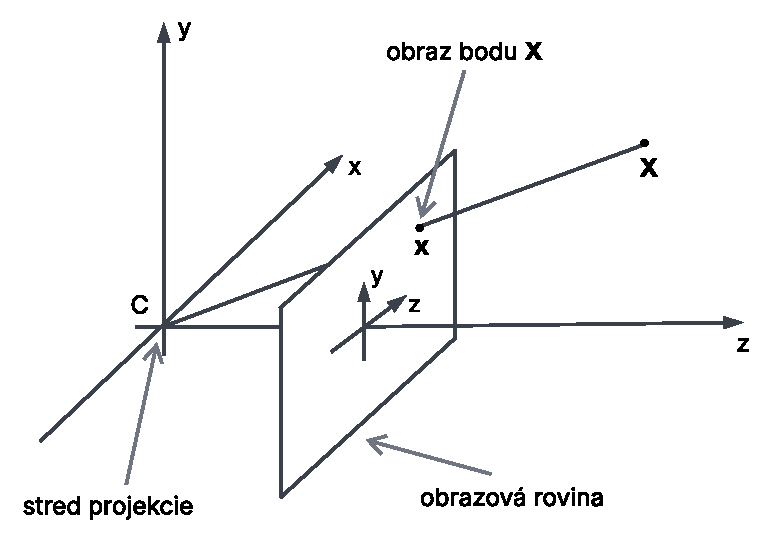
\includegraphics[width=0.7\linewidth]{text_prace/obrazky-figures/model_kamery1.pdf}
    \caption[Zakladný princíp dierkového modelu kamery.]{Zakladný princíp dierkového modelu kamery. Prevzaté z~\cite{multiple_view_geometry}.}
    \label{fig:model_kamery1}
\end{figure}

\begin{figure}[h!]
    \centering
    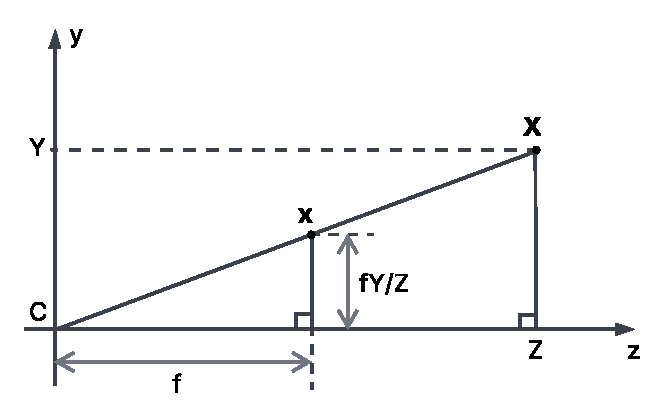
\includegraphics[width=0.7\linewidth]{text_prace/obrazky-figures/model_kamery2.pdf}
    \caption[Náčrt odvodenia súradníc zobrazovaného bodu u~dierkového modelu kamery.]{Náčrt odvodenia súradníc bodu $\mathbf{x}$. Prevzaté z~\cite{multiple_view_geometry}.}
    \label{fig:model_kamery2}
\end{figure}

Keďže všetky obrazy bodov ležia v~obrazovej rovine $z = f$, je možné poslednú súradnicu zanedbať a zapisovať súradnice bodu $\mathbf{x}$ v~súradnicovom systéme obrazovej roviny ako $(fX/Z, fY/Z)^T$.

Túto projekciu môžeme v~homogénnych súradniciach zapísať pomocou násobenia matíc nasledovným spôsobom:

$$ \mathbf{x} 
=
\begin{pmatrix}
fX \\
fY \\
Z
\end{pmatrix}
=
\begin{bmatrix}
f &   &   & 0 \\
  & f &   & 0 \\
  &   & 1 & 0
\end{bmatrix}
\begin{pmatrix}
X \\
Y \\
Z \\
1
\end{pmatrix}
=
\begin{bmatrix}
f &   &   & 0 \\
  & f &   & 0 \\
  &   & 1 & 0
\end{bmatrix}
\mathbf{X}
=
\mathrm{P} \mathbf{X}
$$

Maticu $\mathrm{P}$ nazývame projekčnou maticou kamery (\emph{camera projection matrix}).

\subsubsection{Rozšírenia základného dierkového modelu kamery}

V~praxi väčšinou chceme vyjadriť body na obrazovej rovine v~súradnicovom systéme, ktorý nemá stred v~bode $(0, 0, f)^T$, ale v~ľubovoľnom bode $(-p_x, -p_y, f)^T$ (obrázok \ref{fig:model_kamery3}). Obrazom bodu $\mathbf{X} = (X, Y, Z)^T$ (v~súradnicovom systéme kamery) potom bude bod $\mathbf{x} = (fX/Z + p_x, fY/Z + p_y, f)^T$ (v~súradnicovom systéme obrazovej roviny). To je možné zahrnúť do projekčnej matice nasledovným spôsobom:

$$ \mathrm{P} =
\begin{bmatrix}
f &   & p_x & 0 \\
  & f & p_y & 0 \\
  &   &  1  & 0
\end{bmatrix}
$$

$$ \mathbf{x} 
=
\begin{pmatrix}
fX/Z + p_x \\
fY/Z + p_y \\
1
\end{pmatrix}
=
\begin{pmatrix}
fX + Z p_x \\
fY + Z p_y \\
Z
\end{pmatrix}
=
\begin{bmatrix}
f &   &  p_x & 0 \\
  & f &  p_y & 0 \\
  &   &   1  & 0
\end{bmatrix}
\begin{pmatrix}
X \\
Y \\
Z \\
1
\end{pmatrix}
$$

Maticu

$$ \mathrm{K} 
=
\begin{bmatrix}
f &   &  p_x \\
  & f &  p_y \\
  &   &   1  
\end{bmatrix}
$$

nazývame kalibračnou maticou kamery (\emph{camera calibration matrix}) a medzi ňou a projekčnou maticou platí vzťah
$\mathrm{P} = \begin{bmatrix} \mathrm{K} | 0 \end{bmatrix}$, kde $0$ predstavuje nulový stĺpcový vektor.

\begin{figure}[h!]
    \centering
    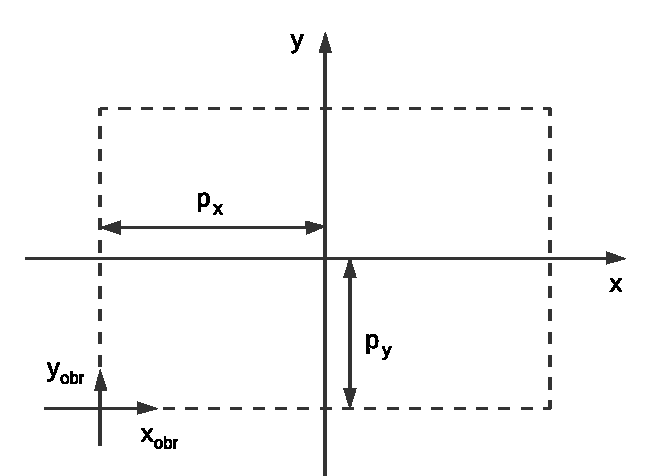
\includegraphics[width=0.7\linewidth]{text_prace/obrazky-figures/model_kamery3.pdf}
    \caption[Súradnicový systém so stredom v~bode $(-p_x, -p_y, f)^T$ obrazovej roviny.]{Súradnicový systém so stredom v~bode $(-p_x, -p_y, f)^T$ obrazovej roviny. Prevzaté z~\cite{multiple_view_geometry}.}
    \label{fig:model_kamery3}
\end{figure}

U~niektorých kamier je možné, že súradnicový systém obrazovej roviny nemá rovnakú mierku na oboch osiach. Vtedy sú v~kalibračnej matici namiesto parametra $f$ parametre $f_x$, $f_y$ a matica má podobu

$$ \mathrm{K'} 
=
\begin{bmatrix}
f_x &     &  p_x \\
    & f_y &  p_y \\
    &     &   1  
\end{bmatrix} \mathrm{.}
$$

Parametre $p_x$, $p_y$ a $f$, prípadne $f_x$ a $f_y$ označujeme ako \textbf{vnútorné parametre kamery}.

Až doteraz sme predpokladali, že kamera má stred v~počiatku súradnicovej sústavy a je \uv{otočená} v~smere osi $z$, t. j. že obrazová rovina je rovnobežná s~rovinou $xy$. V~praxi to tak však nebýva a kamera má v~súradnicovom systéme, v~ktorom sú definované zobrazované body, istú rotáciu a transláciu. V~takom prípade rozlišujeme všeobecný súradnicový systém a súradnicový systém kamery (\emph{world coordinate frame} a \emph{camera coordinate frame}).

Ak $\widetilde{\mathbf{X}}$ je vektor súradníc bodu $\mathbf{X}$ vo všeobecnom súradnicovom systéme a vektor $\widetilde{\mathbf{X}}_{\mathrm{cam}}$ reprezentuje ten istý bod v~súradnicovom systéme kamery, tak platí vzťah 
$$\widetilde{\mathbf{X}}_{\mathrm{cam}} = \mathrm{R} (\widetilde{\mathbf{X}} - \widetilde{\mathbf{C}}),$$ 
kde $\widetilde{\mathbf{C}}$ sú súradnice stredu kamery vo všeobecnom súradnicovom systéme a $\mathrm{R}$ je rotačná matica $3 \times 3$ reprezentujúca orientáciu súradnicového systému kamery. To vedie k~novému vyjadreniu projekčnej matice ako $\mathrm{P} = \mathrm{K} \mathrm{R} \bigl[ \mathrm{I} | - \widetilde{\mathbf{C}} \bigr]$, kde $\mathrm{I}$ je jednotková matica $3 \times 3$.

Parametre $\mathrm{R}$ a $\widetilde{\mathbf{C}}$ označujeme ako \textbf{vonkajšie parametre kamery}.

\section{Skreslenie kamery}
\label{sec:skreslenie}

Dierkový model kamery zodpovedá spôsobu, akým zachytávajú obraz reálne kamery, iba približne, ale nie presne. Obraz z~reálnej kamery má zvyčajne navyše ešte skreslenie.

Existujú rôzne modely skreslenia, z~ktorých najčastejšie používané sú radiálne skreslenie (\emph{radial distortion}) a tangenciálne skreslenie (\emph{tangential/decentering distortion}) \cite{sun_cooperstock_camera_calibration}.

Radiálne skreslenie vzniká v~dôsledku rozdielneho lomu lúčov v~strede a na okraji šošovky a je tým väčšie, čím menšia je šošovka. Príklad radiálneho skreslenia je na obrázku \ref{fig:radialne_skreslenie}. Tangenciálne skreslenie vzniká vtedy, keď šošovka nie je rovnobežná s~obrazovou rovinou~\cite{matlab_camera_calibration}. Reálne kamery zvyčajne majú radiálne skreslenie väčšie než tangenciálne \cite{opencv_camera_calibration_older}.

Radiálne skreslenie sa počíta vzťahmi

$$x_{distorted} = x(1 + k_1 r^2 + k_2 r^4 + k_3 r^6)$$
$$y_{distorted} = y(1 + k_1 r^2 + k_2 r^4 + k_3 r^6)$$

kde

\begin{itemize}
    \item $x, y$ sú normalizované obrazové súradnice (\emph{normalized image coordinates}) bodu pred skreslením,
    \item $k_1, k_2, k_3$ sú koeficienty radiálneho skreslenia,
    \item $r^2 = x^2 + y^2$ \cite{opencv_camera_calibration}.
\end{itemize}

Normalizovaný obrazový súradnicový systém je súradnicový systém, ktorý má tieto vlastnosti:
\begin{itemize}
    \item Jeho stred je v~strede obrazu,
    \item Väčšia dimenzia obrazu má veľkosť 1.
\end{itemize}

Teda napríklad obraz s~pomerom strán 4:3 bude v~normalizovanom obrazovom súradnicovom systéme obdĺžnik s~ľavým dolným rohom v~bode $[-0.5, 3/4 \times (-0.5)]$ a pravým horným rohom v~bode $[0.5, 3/4 \times 0.5]$.

Prevod zo súradníc pixelu v~obraze s~rozlíšením $w \times h$ pixelov do normalizovaných obrazových súradníc je nasledovný \cite{opensfm_coordinate_systems}:

$$
x_{norm} = \frac{x_{pix} - \frac{w-1}{2}}{max(w, h)}
\mathrm{,} \quad
y_{norm} = \frac{y_{pix} - \frac{h-1}{2}}{max(w, h)}
\mathrm{.}
$$

Tangenciálne skreslenie sa počíta vzťahmi

$$x_{distorted} = x + [2 p_1 x y + p_2(r^2 + 2 x^2)]$$
$$y_{distorted} = y + [ p_1(r^2 + 2 y^2) + 2 p_2 x y]$$

kde

\begin{itemize}
    \item $x, y, r^2$ sú rovnaké ako u~radiálneho skreslenia,
    \item $p_1, p_2$ sú koeficienty tangenciálneho skreslenia \cite{opencv_camera_calibration}.
\end{itemize}

Vzťahy pre výpočet radiálneho a tangenciálneho skreslenia zároveň sú nasledovné \cite{sun_cooperstock_camera_calibration}:

$$x_{distorted} = x(1 + k_1 r^2 + k_2 r^4 + k_3 r^6) + [2 p_1 x y + p_2(r^2 + 2 x^2)]$$
$$y_{distorted} = y(1 + k_1 r^2 + k_2 r^4 + k_3 r^6) + [ p_1(r^2 + 2 y^2) + 2 p_2 x y]$$

Koeficienty skreslenia sa zvyčajne udávajú ako pätica \cite{opencv_camera_calibration}

$$(k_1, k_2, p_1, p_2, k_3)\mathrm{.}$$

Proces zisťovania parametrov kamery, vrátane koeficientov skreslenia, sa nazýva kalibrácia kamery (\emph{camera calibration}) \cite{matlab_camera_calibration}.

\begin{figure}[t]
    \centering
    
\includegraphics[width=0.6\linewidth]{text_prace/obrazky-figures/radialne_skreslenie.png}
    \caption[Radiálne skreslenie kamery ilustrované na mriežke.]{Radiálne skreslenie ilustrované na mriežke. Bledomodrá mriežka je pôvodná, čierna skreslená. Pri tvorbe obrázku boli použité skutočné parametre radiálneho skreslenia kamery mobilného mapovacieho systému, ktoré boli súčasťou dát dodaných k~tvorbe tejto práce: $k_1 = -0.183217$, $k_2 = 0.026917$, $k_3 = 0.335446$}.
    \label{fig:radialne_skreslenie}
\end{figure}

\section{Vykresľovací reťazec}

Proces vykresľovania trojrozmerných objektov na dvojrozmernú obrazovku v~počítačovej grafike pozostáva z~viacerých transformácií. Vykresľované objekty sú postupne prevádzané cez niekoľko súradnicových systémov pomocou transformačných matíc.

Abstraktný model, ktorý popisuje sériu krokov potrebných k~zobrazeniu trojrozmernej scény zloženej z~viacerých objektov, sa nazýva vykresľovací reťazec (\emph{graphics/rendering pipeline}). Vykresľovací reťazec zahŕňa popis prenosu dát na grafickú kartu, výpočet finálnej polohy objektu na obrazovke, rasterizáciu (určenie, ktoré pixely zodpovedajú vektorovo popísaným objektom) a výpočet farby pixelov \cite{stemkoski_graphics}.

Vykresľovací reťazec môže mať rôzne podoby. V~tejto sekcii je popísaná verzia, ktorú používa knižnica OpenGL, pretože, ako bude popísané v~sekcii \ref{sec:deck_gl}, pri implementácii tejto práce bol použitý framework, ktorý používa rozhranie WebGL, ktoré je založené práve na knižnici OpenGL \cite{webgl_overview}.

Vykresľované objekty sa typicky skladajú z~bodov (\emph{vertices}) pospájaných hranami do trojuholníkov \cite{stemkoski_graphics}. Táto sekcia sa bude zaoberať iba popisom transformácie bodov z~lokálneho súradnicového systému do finálnej polohy vo vykreslenom obraze.

Na začiatku vykresľovacieho reťazca sú body v~lokálnom súradnicovom systéme (\emph{\mbox{local}/ object space}, každý objekt má vlastný súradnicový systém), s~homogénnymi súradnicami v~tvare $V_{local} = (x, y, z, 1)^T$. Potom prechádzajú transformáciami, ktoré sa počítajú násobením súradníc bodu maticami a sú znázornené na obrázku \ref{fig:suradnicove_systemy}. Sú to nasledujúce transformácie:

\begin{enumerate}
    \item Modelová transformácia (\emph{model transformation}). Každý objekt vo vykresľovanej scéne má vlastnú modelovú maticu $M_{model}$ (\emph{model matrix}), ktorá popisuje jeho pozíciu, orientáciu a veľkosť v~scéne. Po modelovej transformácii sú súradnice bodov v~súradnicovom systéme scény (\emph{world space}) \cite{de_vries_coordinate_systems, stemkoski_graphics}.
    \item Pohľadová transformácia (\emph{view transformation}). Prevádza body zo súradnicového systému scény do súradnicového systému kamery (\emph{view/camera/eye space}). Zodpovedá jej pohľadová matica $M_{view}$ (\emph{view matrix}), ktorá popisuje polohu a orientáciu kamery v~súradnicovom systéme scény \cite{de_vries_coordinate_systems, stemkoski_graphics}. 
    \item Projekcia (\emph{projection transformation}). Je buď ortografická, alebo perspektívna. Prevádza body zo súradnicového systému kamery do orezávacieho súradnicového systému (\emph{clip space}). Určuje, ktoré body scény budú viditeľné a ktoré nie, pretože sa zobrazia iba body, ktoré budú mať v~orezávacom súradnicovom systéme všetky súradnice v~intervale $(-1, 1)$ \cite{stemkoski_graphics}. Týmto súradniciam sa hovorí aj \emph{normalized device coordinates} (NDC). Oblasť v~súradnicovom systéme scény, ktorá bude vo finálnom obraze viditeľná, sa nazýva \emph{frustum}. U~ortografickej projekcie má tvar kvádra a u~perspektívnej projekcie má tvar zrezaného ihlana \cite{de_vries_coordinate_systems}, čo ilustruje obrázok \ref{fig:perspektivna_projekcia_frustum}. Zodpovedá jej projekčná matica (\emph{projection matrix}), ktorá má tvar 
    $$
    M_{projection} = 
    \begin{pmatrix}
    k_1 & 0 & k_2 & 0 \\
    0 & k_3 & k_4 & 0 \\
    0 & 0 & \frac{-(f+n)}{f-n} & \frac{-2fn}{f-n} \\
    0 & 0 & -1 & 0
    \end{pmatrix}
    \mathrm{,}
    $$
    kde $n$ a $f$ sú vzdialenosti prednej a zadnej orezávacej rovniny (\emph{near plane} a \emph{far plane}, znázornené na obrázku \ref{fig:perspektivna_projekcia_frustum}) \cite{ahn_projection_matrix}. \\ 
    Po vynásobení súradníc bodov projekčnou maticou je potrebné ešte vydeliť ich súradnice v~tvare $(x, y, z, w)^T$ homogénnou zložkou, čím vznikne tvar $(x/w, y/w, z/w, 1)^T$ aby bolo možné zistiť, či sú všetky súradnice v~intervale $(-1, 1)$, a teda či bude bod súčasťou výsledného obrazu. Táto operácia sa nazýva perspektívne delenie (\emph{perspective division}) \cite{de_vries_coordinate_systems}.  
    \item Transformácia do súradnicového systému obrazu (\emph{viewport transform}). Prevádza body z~orezávacieho súradnicového systému do súradnicového systému finálneho obrazu (\emph{\mbox{screen} space}) \cite{de_vries_coordinate_systems}. Matica, ktorá vykonáva túto transformáciu, sa nazýva \emph{viewport transform matrix} a má tvar
    $$
    M_{viewport} = 
    \begin{pmatrix}
    \frac{w}{2} & 0 & 0 & \frac{w}{2} \\
    0 & \frac{h}{2} & 0 & \frac{h}{2} \\
    0 & 0 & \frac{f-n}{2} & \frac{f+n}{2} \\
    0 & 0 & 0 & 1
    \end{pmatrix}
    \mathrm{,}
    $$
    kde $w$ a $h$ je výška a šírka obrazu v~pixeloch \cite{ahn_viewport_transform}.
\end{enumerate}

\begin{figure}[t]
    \centering
    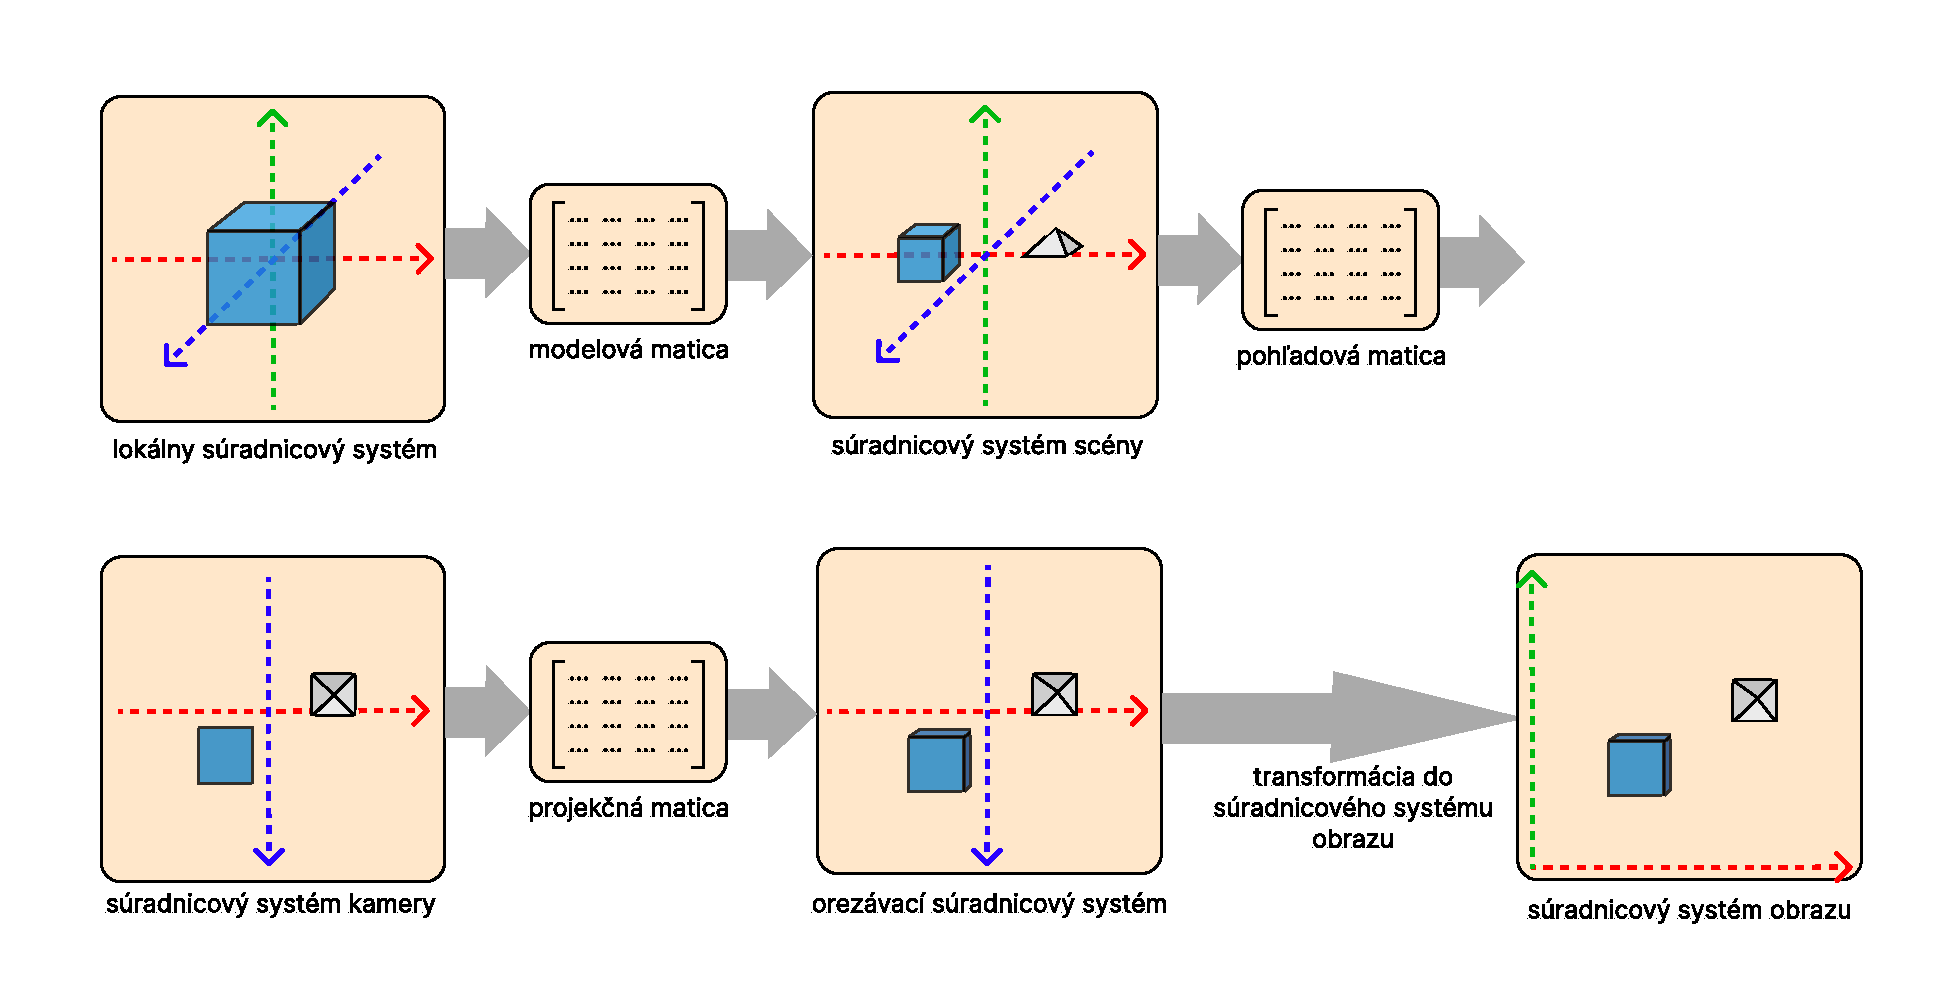
\includegraphics[width=1\linewidth]{text_prace/obrazky-figures/suradnicove_systemy.pdf}
    \caption[Transformácie medzi rôznymi súradnicovými systémami, ktoré sú súčasťou vykresľovacieho reťazca.]{Transformácie medzi rôznymi súradnicovými systémami, ktoré sú súčasťou vykresľovacieho reťazca. Prevzaté z~\cite{de_vries_coordinate_systems}.}
    \label{fig:suradnicove_systemy}
\end{figure}

\begin{figure}[h!]
    \centering
    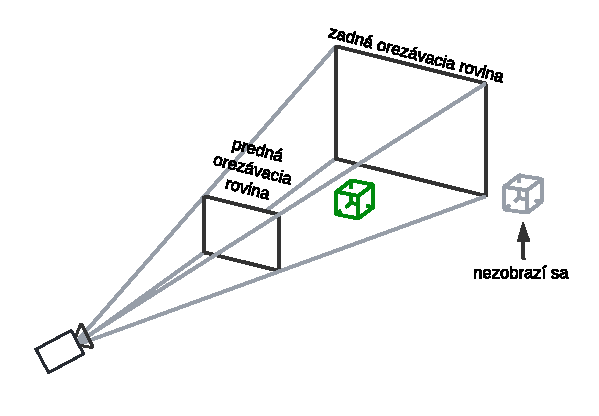
\includegraphics[width=0.6\linewidth]{text_prace/obrazky-figures/perspektivna_projekcia_frustum.pdf}
    \caption[Frustum u~perspektívnej projekcie.]{\emph{Frustum} -- oblasť v~súradnicovom systéme scény, ktorá bude vo finálnom obraze viditeľná -- u~perspektívnej projekcie. Prevzaté z~\cite{de_vries_coordinate_systems}.}
    \label{fig:perspektivna_projekcia_frustum}
\end{figure}

Pozíciu bodu $V_{local}$ vo finálnom vykreslenom obraze scény je teda možné matematicky vyjadriť ako súčin

$$ M_{viewport} \cdot M_{projection} \cdot M_{view} \cdot M_{model} \cdot V_{local} \mathrm{.}$$

Transformácia z~lokálneho súradnicového systému do NDC prebieha na programovateľnej časti grafickej karty, ktorá sa nazýva \emph{vertex shader} \cite{de_vries_coordinate_systems}.

\subsubsection{Vzťah vykresľovacieho reťazca k~dierkovému modelu kamery}

Vykresľovací reťazec a dierkový model kamery sú modely, ktoré sú si podobné, pretože sa oba zaoberajú transformáciou trojrozmernej scény do dvojrozmerného obrazu. Používajú sa však v~odlišných oblastiach -- dierkový model kamery sa typicky používa v~teórii počítačového videnia a vykresľovací reťazec sa týka počítačovej grafiky a zobrazovania trojrozmerných modelov.

Rozdiely a podobnosti oboch modelov je možné zhrnúť týmito bodmi:
\begin{itemize}
    \item Dierkový model kamery nemá nič zodpovedajúce modelovej transformácii. Zobrazované body sú už od začiatku v~rovnakom súradnicovom systéme ako kamera.
    \item Pohľadová transformácia zodpovedá vonkajším parametrom kamery.
    \item Vnútorné parametre kamery zodpovedajú projekcii a transformácii do súradnicového systému obrazu. Vykresľovací reťazec má špeciálny medzistupeň -- orezávací súradnicový systém, ktorý dierkový model kamery nemá.
    \item Dierkový model kamery je jednoduchší, pretože na rozdiel od vykresľovacieho reťazca nemá prednú a zadnú orezávaciu rovinu a nerieši prekrývanie objektov. Vykreľovací reťazec ponecháva aj vo finálnych súradniciach bodu v~obraze hodnotu $z$, teda hĺbku, aby u~prekrývajúcich sa objektov bolo možné zistiť, ktorý z~nich je v~popredí. Dierkový model kamery nič také nezahŕňa.
\end{itemize}

Za poznámku stojí, že v~oboch modeloch sa vyskytuje termín \emph{projekčná matica}, ale ide o~dve rôzne matice.

V~rámci tejto práce bolo potrebné skombinovať znalosti z~oboch oblastí, pretože súčasťou dodaných dát bola kalibračná matica kamery, pomocou ktorej mali byť dáta zobrazené, ale použitý framework si vyžadoval zadať projekčnú maticu (tú z~vykresľovacieho reťazca).

Problém sa dá formulovať nasledovne: je známa projekčná matica (tá z~dierkového modelu kamery), ktorá prevádza body zo súradnicového systému kamery priamo do súradnicového systému obrazu, pričom nepočíta hodnotu hĺbky. Je potrebné vypočítať projekčnú maticu, ktorá bude prevádzať body zo súradnicového systému kamery do orezávacieho súradnicového systému tak, aby následne po automatickom prevode do súradnicového systému obrazu výsledný obraz zodpovedal zadanej projekčnej matici. Rozmery $w \times h$ výsledného obrazu sú známe.

Riešenie je možné matematicky odvodiť. Známa projekčná matica, ktorá prevádza body priamo do súradnicového systému obrazu, má tvar

$$ \mathrm{P} =
\begin{pmatrix}
f_x & 0 & p_x & 0 \\
0 & f_y & p_y & 0 \\
0 & 0 &  1  & 0
\end{pmatrix} \mathrm{.}
$$

Potrebujeme nájsť maticu $M_{projection}$ takú, aby platila rovnosť

$$M_{viewport} \cdot M_{projection} \cdot V_{view} = P \cdot V_{view} \mathrm{,}$$

teda parametre $k_1$, $k_2$, $k_3$ a $k_4$ také, aby platila rovnosť

$$
\begin{pmatrix}
\frac{w}{2} & 0 & 0 & \frac{w}{2} \\
0 & \frac{h}{2} & 0 & \frac{h}{2} \\
0 & 0 & \frac{f-n}{2} & \frac{f+n}{2} \\
0 & 0 & 0 & 1
\end{pmatrix}
\cdot
\begin{pmatrix}
k_1 & 0 & k_2 & 0 \\
0 & k_3 & k_4 & 0 \\
0 & 0 & \frac{-(f+n)}{f-n} & \frac{-2fn}{f-n} \\
0 & 0 & -1 & 0
\end{pmatrix}
\cdot
\begin{pmatrix}
x \\
y \\
z \\
1
\end{pmatrix}
=
\begin{pmatrix}
f_x & 0 & p_x & 0 \\
0 & f_y & p_y & 0 \\
? & ? & ? & ? \\
0 & 0 &  1  & 0
\end{pmatrix}
\cdot
\begin{pmatrix}
x \\
y \\
z \\
1
\end{pmatrix} \mathrm{.}
$$

Otázniky pridané do matice $P$ zastupujú výpočet súradnice $z$, ktorý pôvodná matica neobsahovala, ale pri vykresľovaní trojrozmenej scény v~počítačovej grafike je nutný.

Rovnosť zjednodušíme
$$
\begin{pmatrix}
\frac{w}{2} & 0 & 0 & \frac{w}{2} \\
0 & \frac{h}{2} & 0 & \frac{h}{2} \\
0 & 0 & \frac{f-n}{2} & \frac{f+n}{2} \\
0 & 0 & 0 & 1
\end{pmatrix}
\cdot
\begin{pmatrix}
k_1 x + k_2 z \\
k_3 y + k_4 z \\
\frac{-(f+n)}{f-n} z + \frac{-2fn}{f-n} \\
-z
\end{pmatrix}
=
\begin{pmatrix}
f_x x + p_x z \\
f_y y + p_y z \\
? z + ? \\
z
\end{pmatrix} \mathrm{,}
$$

vykonáme delenie homogénnou súradnicou

$$
\begin{pmatrix}
\frac{w}{2} & 0 & 0 & \frac{w}{2} \\
0 & \frac{h}{2} & 0 & \frac{h}{2} \\
0 & 0 & \frac{f-n}{2} & \frac{f+n}{2} \\
0 & 0 & 0 & 1
\end{pmatrix}
\cdot
\begin{pmatrix}
- k_1 \frac{x}{z} - k_2 \\
- k_3 \frac{y}{z} - k_4 \\
\frac{(f+n)}{f-n} + \frac{2fn}{z(f-n)} \\
1
\end{pmatrix}
=
\begin{pmatrix}
f_x \frac{x}{z} + p_x \\
f_y \frac{y}{z} + p_y \\
? + \frac{?}{z} \\
1
\end{pmatrix}
$$

a znova zjednodušíme

$$
\begin{pmatrix}
\frac{w}{2} (- k_1 \frac{x}{z} - k_2) + \frac{w}{2} \\
\frac{h}{2} (- k_3 \frac{y}{z} - k_4) + \frac{h}{2} \\
\frac{f-n}{2} (\frac{(f+n)}{f-n} + \frac{2fn}{z(f-n)}) + \frac{f+n}{2} \\
1
\end{pmatrix}
=
\begin{pmatrix}
f_x \frac{x}{z} + p_x \\
f_y \frac{y}{z} + p_y \\
? + \frac{?}{z} \\
1
\end{pmatrix}
$$

$$
\begin{pmatrix}
- k_1 \frac{w}{2} \frac{x}{z} - k_2 \frac{w}{2} + \frac{w}{2} \\
- k_3 \frac{h}{2} \frac{y}{z} - k_4 \frac{h}{2} + \frac{h}{2} \\
f + n + \frac{fn}{z} \\
1
\end{pmatrix}
=
\begin{pmatrix}
f_x \frac{x}{z} + p_x \\
f_y \frac{y}{z} + p_y \\
? + \frac{?}{z} \\
1
\end{pmatrix}
$$

$$
\begin{pmatrix}
- k_1 \frac{w}{2} \frac{x}{z} + \frac{w}{2} (1 - k_2)\\
- k_3 \frac{h}{2} \frac{y}{z} + \frac{h}{2} (1 - k_4)\\
f + n + \frac{fn}{z} \\
1
\end{pmatrix}
=
\begin{pmatrix}
f_x \frac{x}{z} + p_x \\
f_y \frac{y}{z} + p_y \\
? + \frac{?}{z} \\
1
\end{pmatrix} \mathrm{.}
$$

Z~toho vyplýva, že parametre $n$ a $f$ je možné si zvoliť ľubovoľne, pretože ich zadaná matica nedefinuje, a že musí platiť

$$
-k_1 \frac{w}{2} = f_x 
\mathrm{,} \quad
\frac{w}{2} (1 - k_2) = p_x \mathrm{,}
$$
$$
-k_3 \frac{h}{2} = f_y
\mathrm{,} \quad
\frac{h}{2} (1 - k_4) = p_y \mathrm{,}
$$

a teda sme dospeli k~hľadanému vyjadreniu parametrov $k_1$, $k_2$, $k_3$ a $k_4$

$$
k_1 = - \frac{2 f_x}{w}
\mathrm{,} \quad
k_2 = 1 - \frac{2 p_x}{w} \mathrm{,}
$$
$$
k_3 = - \frac{2 f_y}{h}
\mathrm{,} \quad
k_4 = 1 - \frac{2 p_x}{w} \mathrm{.}
$$

Hľadaná projekčná matica má teda tvar

$$
M_{projection}
=
\begin{pmatrix}
- \frac{2 f_x}{w} & 0 & 1 - \frac{2 p_x}{w} & 0 \\
0 & - \frac{2 f_y}{h} & 1 - \frac{2 p_x}{w} & 0 \\
0 & 0 & \frac{-(f+n)}{f-n} & \frac{-2fn}{f-n} \\
0 & 0 & -1 & 0
\end{pmatrix} \mathrm{.}
$$

\section{Framework deck.gl a jeho nadstavba Pydeck}
\label{sec:deck_gl}

Pri vývoji webovej aplikácie pre vizualizáciu väčšieho množstva dát, u~ktorej má vykresľovanie prebiehať na strane klienta, teda vo webovom prehliadači, sa hodí priamo či nepriamo použiť niektorý z~frameworkov pre zobrazovanie dát v~jazyku JavaScript.

Takým vhodným frameworkom je napríklad deck.gl, ktorý je určený na zobrazovanie veľkých sád dát. Je zameraný najmä na zobrazovanie geografických dát mapových podkladoch, ale hodí sa aj na iné typy dát. Vyznačuje sa vysokou presnosťou a výkonnosťou. Pre akceleráciu využíva rozhrania WebGPU a WebGL2 \cite{deck.gl_documentation}.

Vizualizácia dát v~deck.gl sa skladá z~dvoch základných častí:
\begin{itemize}
    \item Vrstvy (\texttt{Layers}). Do vrstiev sa ukladajú zobrazované dáta. Framework deck.gl ponúka vyše 30 preddefinovaných typov vrstiev, ktoré zodpovedajú rôznym často sa vyskytujúcim typom dát. Pre túto prácu je významná najmä vrstva \texttt{PointCloudLayer}, ktorá je určená na zobrazenie mračna bodov, a vrstva \texttt{PathLayer}, ktorá je určená na zobrazenie trás.
    \item Pohľad (\texttt{View}). Definuje vlastnosti kamery, napríklad zorné pole a prednú a zadnú orezávaciu rovinu (\emph{near plane} a \emph{far plane}). Je možné buď určiť všetky tieto vlastnosti osobitne, alebo rovno zadať vypočítanú projekčnú maticu.
    Časť \texttt{ViewState} určuje polohu a orientáciu kamery, pričom u~orientácie je možné určiť iba dva uhly (\emph{bearing} a \emph{pitch}). Typ pohľadu definuje spôsob interakcie vizualizácie s~používateľom, napríklad pre zobrazenie trate z~pohľadu strojvedúceho je ideálny typ \texttt{FirstPersonView}.
\end{itemize}

To, že sa deck.gl na vizualizáciu dát z~mobilného mapovacieho systému naozaj hodí, dokazujú ukážky na jeho webových stránkach. Použiteľnosť vrstvy \texttt{PointCloudLayer} demonštruje plynulá animácia mračna vyše 800~000 bodov.

Na webových stránkach deck.gl sa nachádza aj galéria projektov vytvorených pomocou tohto frameworku. Medzi nimi je Autonomous Visualization System (AVS), toolkit pre vývoj webových aplikácií pre vizualizáciu dát z~autonómnych vozidiel \cite{avs}. Na webových stránkach tohto projektu je ukážka takej aplikácie, ktorá je podobná aplikácii vyvíjanej v~rámci tejto práce. Bližší popis AVS sa nachádza v~sekcii \ref{sec:existujuce_riesenia}.

Hoci je framework deck.gl primárne určený pre použitie v~Javascripte, je možné ho použiť aj v~jazyku Python, a to pomocou knižnice \textbf{Pydeck}. Tá je pomerne jednoduchá a podstatou jej činnosti je, že prevedie kód napísaný v~jazyku Python do formátu JSON. Framework deck.gl má totiž modul @deck.gl/json, ktorý prijíma reprezentáciu vizualizácie vo formáte JSON a transformuje ju do javascriptového kódu (na definície funkcií a deck.gl objektov)\footnote{Ukážka rozhrania modulu @deck.gl/json je na \url{https://deck.gl/playground}.}.

Knižnica Pydeck je dobrým prostriedkom na vytvorenie jednoduchých vizualizácií, s~ktorými môže používateľ interagovať pohybmi myši. Jej možnosti sú však oproti pôvodnému frameworku deck.gl veľmi obmedzené. Nie je vhodná na vytváranie zložitejších animácií s~veľkým množstvom dát, pretože sa aj po tej najmenšej zmene musia dáta a definícia vizualizácie nanovo prevádzať do formátu JSON a následne na javascriptový kód (obrázok \ref{fig:pydeck_dashdeck_schema}), čo je veľmi časovo náročné.

\begin{figure}[h]
    \centering
    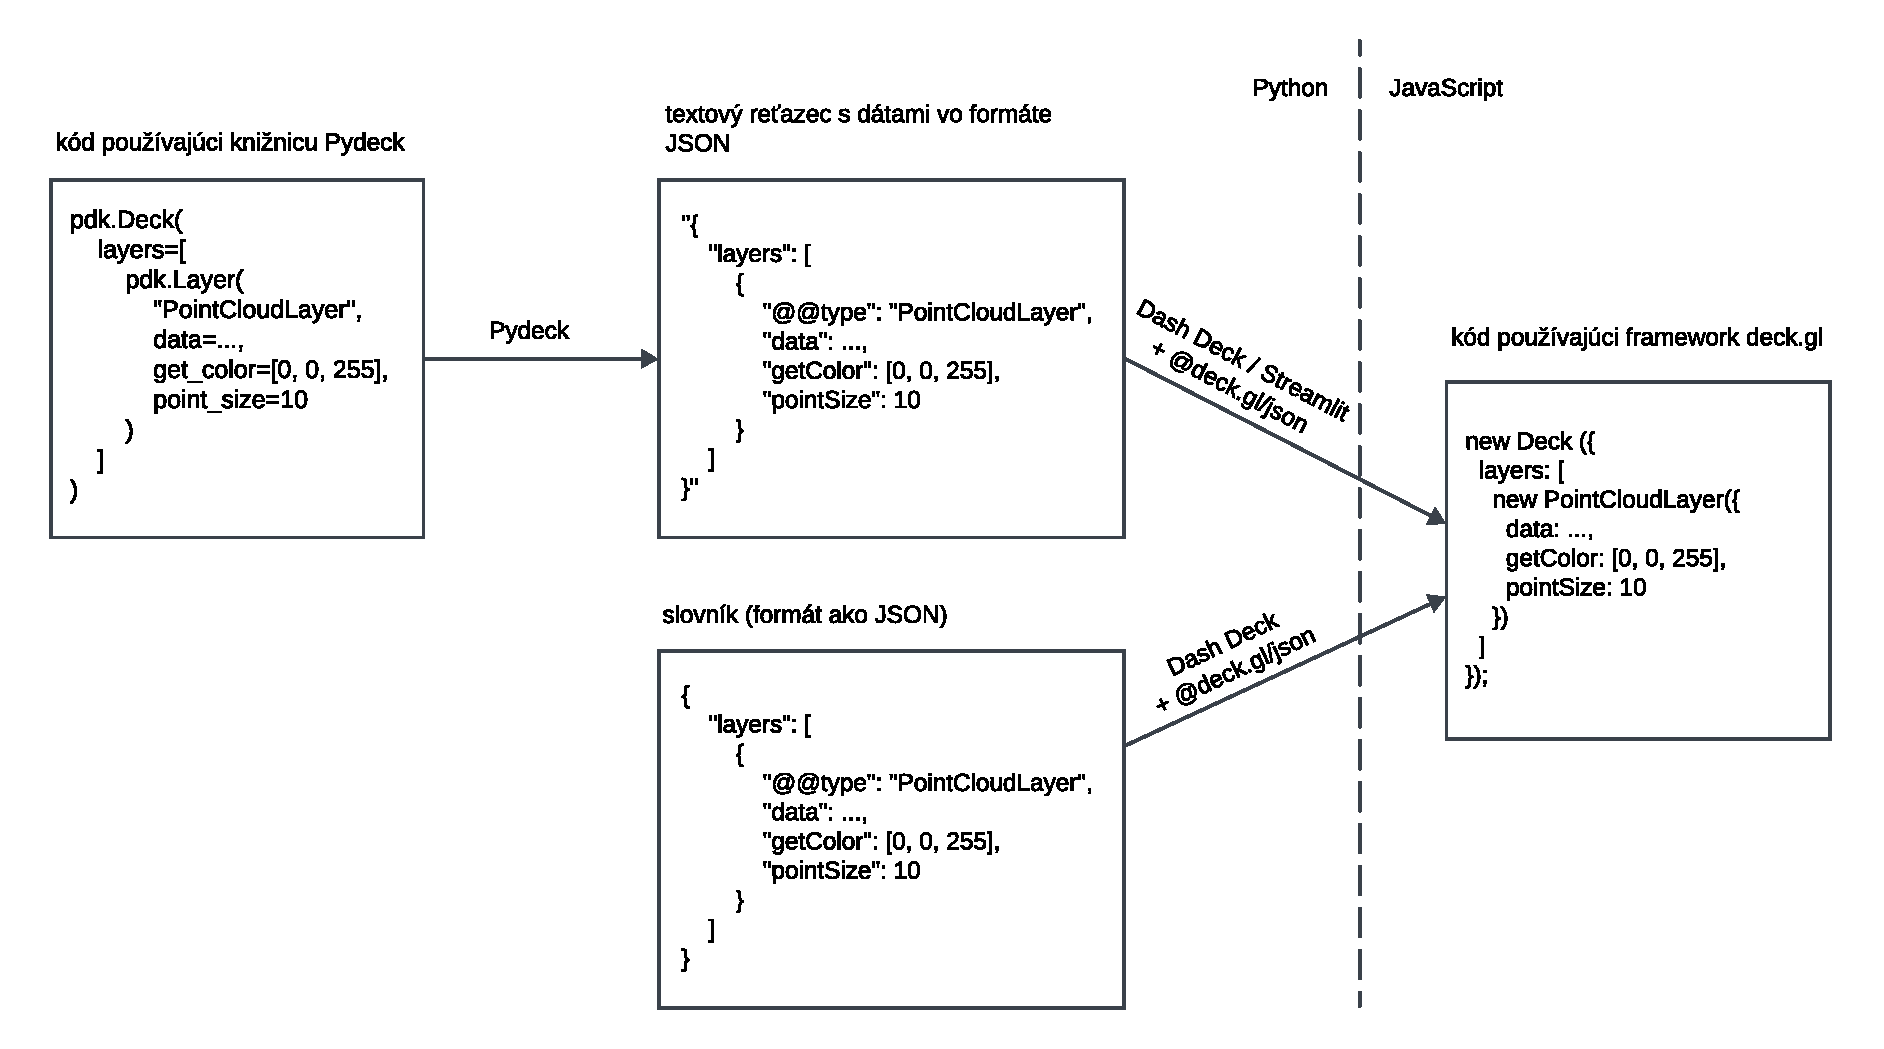
\includegraphics[width=1\linewidth]{text_prace/obrazky-figures/pydeck_dashdeck_transformacie.pdf}
    \caption[Schéma vzťahov medzi technológiami Pydeck, Dash Deck a deck.gl.]{Schéma vzťahov medzi technológiami Pydeck, Dash Deck a deck.gl a transformácií, ktorými prechádza definícia zobrazenia.}
    \label{fig:pydeck_dashdeck_schema}
\end{figure}

\section{Nastavenie polohy kamery vo frameworku deck.gl}
\label{sec:nastavenie_polohy_kamery}

Súčasťou dodaných dát z~mobilného mapovacieho systému boli rotácie a translácie kamery. Pre nastavenie polohy vo frameworku deck.gl existujú dve možnosti:

\begin{enumerate}
    \item Aplikovať transformáciu na dáta a nechať kameru v~počiatku súradnicového systému, prípadne v~nejakom inom pevnom bode.
    \item Nechať dáta v~pôvodnom stave a aplikovať všetky transformácie iba na kameru.
\end{enumerate}

Je zrejmé, že pre dosiahnutie rovnakého výsledku musí byť transformácia použitá v~druhom prípade inverzná k~tej, ktorá je použitá v~tom prvom.

Bližším popisom a zhodnotením výhod a nevýhod týchto dvoch metód sa zaoberajú nasledujúce dve podsekcie.

\subsubsection{Aplikovanie transformácií na dáta}

Ako bolo zmienené v~sekcii \ref{sec:deck_gl}, dáta sa vo frameworku deck.gl členia do vrstiev. Každej vrstve je potom potrebné priradiť pole s~dátami a definovať pre ňu takzvané prístupové funkcie (\emph{data accessors}), ktoré určujú, akým spôsobom sa z~poľa s~dátami získa poloha a farba prvku. Napríklad u~vrstvy \texttt{PointCloudLayer} je potrebné definovať funkciu \texttt{getPosition} pre získanie polohy bodu a \texttt{getColor} pre výpočet farby bodu \cite{deck.gl_documentation}.

Práve vo funkcii \texttt{getPosition} je možné aplikovať na polohu bodu ľubovoľnú transformáciu.

Napríklad v~prípade, že je potrebné posunúť kameru v~mračne bodov o~10 jednotiek v~kladnom smere po osi x, by bolo možné vykonať túto transformáciu pomocou funkcie \texttt{getPosition} tak, že by sa posunul každý bod po osi x o~10 jednotiek v~zápornom smere. V~prípade, že by bol v~poli dát každý bod vo formáte \texttt{[x, y, z, intenzita]}, by potom funkcia \texttt{getPosition} vyzerala takto:

\begin{lstlisting}
function getPosition(d) {
  return [d[0] - 10, d[1], d[2]];
}
\end{lstlisting}

Výhodou tohto prístupu je, že je možné vykonať ľubovoľnú transformáciu, pretože do funkcie možno napísať akýkoľvek kód.

Veľkou nevýhodou je časová náročnosť, pri zmene polohy kamery sa totiž musí prepočítať poloha každého bodu. Tieto výpočty sa vykonávajú na procesore a výsledky sa následne nahrávajú na grafickú kartu. To konštatuje aj samotná dokumentácia frameworku deck.gl, kde sa píše, že kľúčom k~tvorbe výkonných aplikácií je minimalizácia aktualizácií vrstiev, pri ktorých dochádza k~prepočítavaniu dát a ich opätovnému nahrávaniu na grafickú kartu. Taktiež je tam uvedené, že prístupové funkcie by mali byť čo najtriviálnejšie, pretože sa počítajú pre každú položku v~dátach, t. j. pre každý bod v~mračne bodov, a teda sa každé pridanie operácií naviac výrazne prejaví na výkonnosti. 99\% procesorového času venovaného aktualizácii dát vrstvy sa strávi práve volaním prístupových funkcií \cite{deck.gl_performance_optimization}.

\subsubsection{Aplikovanie transformácií na kameru}

Meniť polohu a orientáciu kamery je v~deck.gl možné pomocou troch parametrov: \texttt{position}, \texttt{bearing} a \texttt{pitch} \cite{deck.gl_documentation}. To sú rotácie iba podľa dvoch osí, a teda nie je možné dosiahnuť všeobecnú rotáciu -- chýba možnosť nastaviť rotáciu okolo tretej osi, takzvaný \emph{roll} uhol.

V~dokumentácii deck.gl je popísaná aj trieda \texttt{Viewport}, u~ktorej je možné namiesto parametrov \texttt{position}, \texttt{bearing} a \texttt{pitch} nastaviť maticu pohľadu \texttt{viewMatrix}, čo znamená možnosť použiť akúkoľvek rotáciu. Problém je však v~tom, že sa v~dokumentácii už nikde nepíše, ako túto triedu použiť. Ide teda o~nezrovnalosť, pravdepodobne pozostatok z~predchádzajúcich verzií deck.gl, kde táto možnosť bola, ale medzičasom bola zrušená. V~aktuálnej verzii je možné túto maticu už iba prečítať, ale nie nahradiť vlastnou.

Nevýhodou tohto spôsobu nastavenia polohy kamery teda je, že sa nedá nastaviť \emph{roll} uhol. Tento problém je však možné vyriešiť trikom, a to otočením HTML elementu \texttt{canvas}, do ktorého deck.gl vykresľuje výsledné zobrazenie, pomocou CSS vlastnosti \texttt{transform}. 

Za poznámku tiež stojí, že ak potrebujeme na kameru aplikovať nejakú zložitejšiu transformáciu než iba jednu rotáciu a posunutie, tak je potrebné odvodiť vzorce, ktorými sa táto zložitejšia transformácia prevedie na parametre \texttt{position}, \texttt{bearing} a \texttt{pitch}. Konrétnym prípadom, ktorý bolo potrebné vyriešiť v~tejto práci, sa zaoberá nasledujúca kapitola.

Veľkou výhodou naopak je, že na rozdiel od predchádzajúceho spôsobu nedochádza k~žianym aktualizáciám vrstiev, teda nie je potrebné prepočítavať polohy bodov na procesore ani ich znova nahrávať na grafickú kartu. Tým sa výrazne zvýši výkonnosť.

\subsubsection{Upresnenie polohy kamery}

Experimentmi s~dodanými dátami sa zistilo, že ak je mračno bodov zobrazené presne podľa dodaných údajov o~polohe a parametroch kamery, výsledné zobrazenie nesedí presne na záber z~kamery. Aby naozaj sedelo, je potrebné pridať isté posunutie kamery. Taká situácia je zjednodušene znázornená na obrázku \ref{fig:transformacie_kamery} -- je zadaná translácia $T$ a rotácia $R$, ale kameru je ešte potrebné posunúť doprava transláciou $T'$.

\begin{figure}[h]
    \centering
    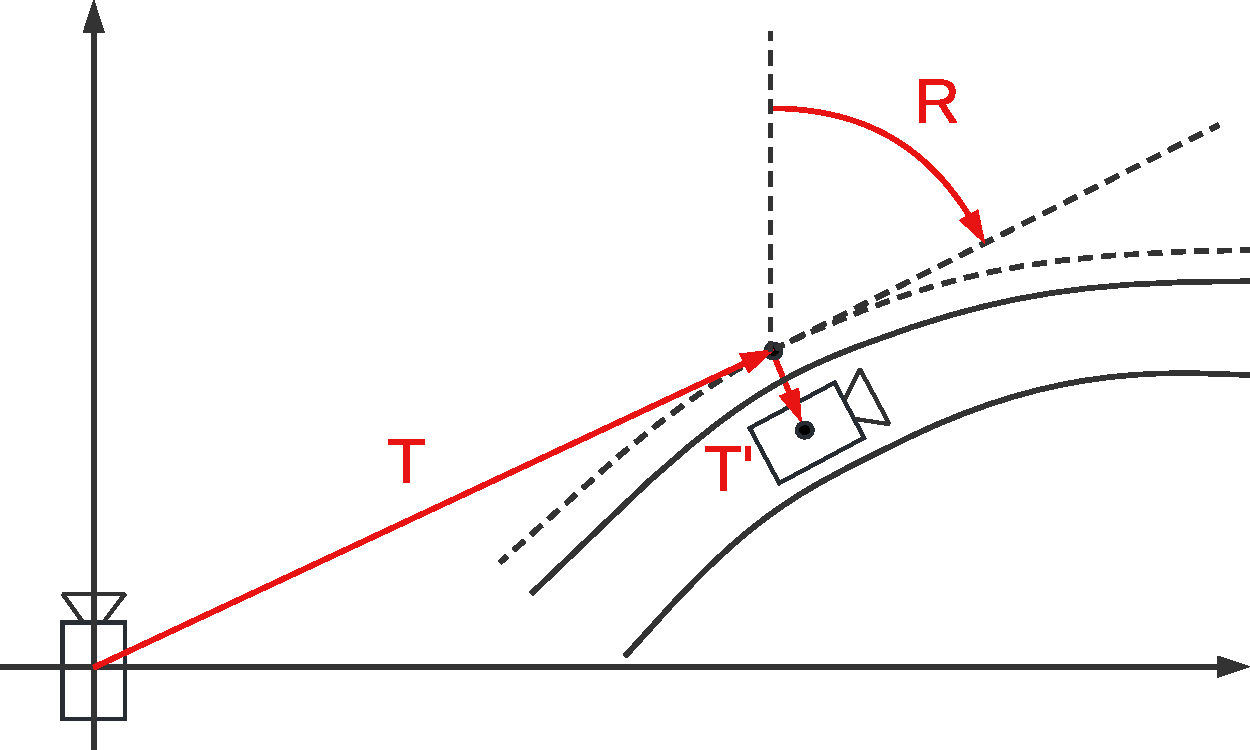
\includegraphics[width=0.8\linewidth]{text_prace/obrazky-figures/tri_transformacie.pdf}
    \caption[Kombinácia viacerých transformácií kamery.]{Zjednodušený príklad situácie, kedy je potrebné kombinovať viacero transformácií kamery. Je k~dispozícii translácia $T$ a rotácia $R$, ale kameru je ešte potrebné posunúť doprava transláciou $T'$, aby bola v~strede koľajníc.}
    \label{fig:transformacie_kamery}
\end{figure}

Ak by bolo pri implementácii v~deck.gl možné použiť aplikovanie transformácií na dáta, mal by tento problém jednoduché riešenie: z~translácie $T$ a rotácie $R$ sa zloží transformačná matica, ktorá sa použije v~prístupovej funkcii, a translácia $T'$ sa priamo použije ako poloha kamery.

Ak však tento prístup nie je vhodný, napríklad z~dôvodu horšieho výkonu, je nutné nájsť transláciu $T_V$ a rotáciu $R_V$ tak, aby platil vzťah 

$$ T R T' = T_V R_V \mathrm{.}$$

Transformácie $T_V$ a $R_V$ sa potom už totiž dajú priamo previesť na parametre \texttt{position}, \texttt{bearing} a \texttt{pitch} (na prevod rotácie na \texttt{bearing} a \texttt{pitch} sa dá použiť napríklad trieda \texttt{Rotation} z~knižnice \texttt{scipy}).

Nech

$$
    T =
    \begin{pmatrix}
    1 & 0 & 0 & t_1 \\
    0 & 1 & 0 & t_2 \\
    0 & 0 & 1 & t_3 \\
    0 & 0 & 0 & 1
    \end{pmatrix}
    \mathrm{,} \quad 
    R =
    \begin{pmatrix}
    r_{11} & r_{12} & r_{13} & 0 \\
    r_{21} & r_{22} & r_{23} & 0 \\
    r_{31} & r_{32} & r_{33} & 0 \\
    0 & 0 & 0 & 1
    \end{pmatrix}
    \mathrm{,} \quad 
    T' =
    \begin{pmatrix}
    1 & 0 & 0 & t'_1 \\
    0 & 1 & 0 & t'_2 \\
    0 & 0 & 1 & t'_3 \\
    0 & 0 & 0 & 1
    \end{pmatrix}
    \mathrm{,}
$$
$$
    T_V =
    \begin{pmatrix}
    1 & 0 & 0 & t_{v1} \\
    0 & 1 & 0 & t_{v2} \\
    0 & 0 & 1 & t_{v3} \\
    0 & 0 & 0 & 1
    \end{pmatrix}
    \quad \mathrm{a} \quad 
    R_V =
    \begin{pmatrix}
    r_{v11} & r_{v12} & r_{v13} & 0 \\
    r_{v21} & r_{v22} & r_{v23} & 0 \\
    r_{v31} & r_{v32} & r_{v33} & 0 \\
    0 & 0 & 0 & 1
    \end{pmatrix}
    \mathrm{.}
$$

Potom

$$
    T R T' =
    \begin{pmatrix}
    r_{11} & r_{12} & r_{13} & t'_1 r_{11} + t'_2 r_{12} + t'_3 r_{13} + t_1 \\
    r_{21} & r_{22} & r_{23} &  t'_1 r_{21} + t'_2 r_{22} + t'_3 r_{23} + t_2 \\
    r_{31} & r_{32} & r_{33} &  t'_1 r_{31} + t'_2 r_{32} + t'_3 r_{33} + t_3 \\
    0 & 0 & 0 & 1
    \end{pmatrix}
$$

a

$$
    T_V R_V =
    \begin{pmatrix}
    r_{v11} & r_{v12} & r_{v13} & t_{v1} \\
    r_{v21} & r_{v22} & r_{v23} & t_{v2} \\
    r_{v31} & r_{v32} & r_{v33} & t_{v3} \\
    0 & 0 & 0 & 1
    \end{pmatrix} \mathrm{.}
$$

Z~toho vyplýva, že musí platiť $R_V = R$ a

$$
    \begin{pmatrix}
    t_{v1} \\
    t_{v2} \\
    t_{v3} \\
    \end{pmatrix}
    =
    \begin{pmatrix}
    t'_1 r_{11} + t'_2 r_{12} + t'_3 r_{13} + t_1 \\
    t'_1 r_{21} + t'_2 r_{22} + t'_3 r_{23} + t_2 \\
    t'_1 r_{31} + t'_2 r_{32} + t'_3 r_{33} + t_3
    \end{pmatrix}
    =
    \begin{pmatrix}
    r_{v11} & r_{v12} & r_{v13} \\
    r_{v21} & r_{v22} & r_{v23} \\
    r_{v31} & r_{v32} & r_{v33}
    \end{pmatrix}
    \begin{pmatrix}
    t'_1 \\
    t'_2 \\
    t'_3
    \end{pmatrix}
    +
    \begin{pmatrix}
    t_1 \\
    t_2 \\
    t_3
    \end{pmatrix} \mathrm{.}
$$

Tým sme našli hľadanú transláciu $T_V$ a rotáciu $R_V$.

\section{Frameworky pre tvorbu webových aplikácií}

Keďže hlavným cieľom práce bolo vytvoriť aplikáciu v~jazyku Python, a to ideálne webovú, bolo potrebné preskúmať existujúce technológie, ktoré to umožňujú.

\subsubsection{Porovnanie frameworkov Streamlit a Dash}

Streamlit a Dash sú frameworky, ktoré majú rovnaké zameranie: oba slúžia na tvorbu webových aplikácií pre prácu s~dátami (\emph{data apps}) v~jazyku Python. Dash je oproti Streamlitu na nižšej úrovni abstrakcie, pretože sám o~sebe nemá žiaden vizuálny štýl a mnohé jeho komponenty sa priamo mapujú na HTML elementy, napríklad \texttt{dash.html.Div} a \texttt{dash.html.H1} \cite{dash_documentation, streamlit_documentation}.

Oba frameworky majú podporu pre Pydeck, u~Streamlitu je priamo k~dispozícii element \texttt{st.pydeck\_chart} a Dash má na tento účel vytvorenú prídavnú knižnicu \textbf{Dash Deck}. Ukázalo sa však, že \texttt{st.pydeck\_chart} podporuje iba pohľad \texttt{MapView}, ktorý je určený na zobrazenie dát na mape a nedá sa použiť na perspektívne zobrazenie bodov v~trojrozmernom priestore. Preto je pre účely tejto práce element \texttt{st.pydeck\_chart} prakticky nepoužiteľný.

Dash Deck má navyše tú výhodu, že umožňuje vynechať Pydeck a definovať zobrazenie iba pomocou slovníkov so štruktúrou zodpovedajúcou tej, ktorú vyžaduje modul @deck.gl/json, čo je tiež znázornené na obrázku \ref{fig:pydeck_dashdeck_schema}. To trochu zefektívni vykonávanie zmien vo vizualizácii, keďže taká reprezentácia umožní jednoduchšie vykonávanie úprav.

Z~týchto dôvodov bol pre implementáciu zvolený framework Dash, ktorý je podrobnejšie popísaný v~nasledujúcej podsekcii.

\subsubsection{Popis frameworku Dash}

Dash je framework, ktorý umožňuje tvorbu webových aplikácií v~jazyku Python. Interne používa na vytváranie používateľského rozhrania framework React \cite{dash_documentation}. Princíp jeho fungovania je nasledovný: kód aplikácie sa spúšťa v~rámci HTTP servera a generuje HTML dokument a skripty v~jazyku JavaScript, ktoré server odošle klientovi. Tieto skripty následne komunikujú sa serverom, čím sa zabezpečuje funkcionalita aplikácie. Server je bezstavový a neuchováva si žiadne informácie o~klientoch.

Kód webovej aplikácie napísanej s~využitím frameworku Dash sa skladá z~dvoch základných častí: komponentov a callbackov.

\emph{Komponenty} sú prvky používateľského rozhrania, ktoré sa skladajú do stromovej štruktúry. Je možné použiť komponenty priamo zodpovedajúce HTML elementom (Dash HTML Components), komponenty z~knižnice Dash Core Components (napríklad \texttt{Graph}, \texttt{Input}, \texttt{Tabs}, \texttt{Upload}) a ďalšie špeciálne komponenty \cite{dash_documentation}.

Pre túto prácu je významný komponent sklad (\texttt{Store}) z~knižnice Dash Core Components, ktorý umožňuje uložiť dáta na strane klienta. Hodí sa na uloženie dát, ktoré sa následne zobrazujú pomocou frameworku deck.gl.

Ďalej je možné použiť knižnicu \textbf{Dash Bootstrap Components} (DBC), ktorá poskytuje ďalšie komponenty, ikony, lepšie možnosti pre rozloženie stránky, a v~neposlednom rade vizuálne štýly \cite{dbc_documentation}.

Tam, kde nestačia štýly a možnosti rozloženia stránky z~DBC, je možné u~komponentov dodefinovať vlastné pravidlá v~jazyku CSS.

\emph{Callbacky} vytvárajú funkcionalitu aplikácie. Každý callback je funkcia, ktorá má vstupy a výstupy. Vstupy a výstupy sú vždy atribúty konkrétnych komponentov. Callback sa zavolá na začiatku behu aplikácie (táto vlastnosť sa dá zrušiť) a potom vždy, keď sa zmení niektorý z~jeho vstupov. Callback môže mať aj špeciálne vstupy typu \texttt{State}, ktorých zmena callback nespustí. Platí obmedzenie, že každý atribút komponentu môže byť výstupom maximálne jedného callbacku \cite{dash_documentation}. U~vstupov žiadne obmedzenia nie sú.

Existujú dva typy callbackov.
\begin{itemize}
    \item Obyčajné callbacky. Sú napísané v~jazyku Python. Klient má iba informáciu o~ich vstupoch a výstupoch. Keď sa zmení niektorý zo vstupov, klient pošle na server požiadavok obsahujúci hodnoty všetkých vstupov. Server spustí kód callbacku a pošle klientovi odpoveď, ktorá obsahuje hodnoty všetkých výstupov.
    \item Klientske callbacky. Sú napísané v~jazyku JavaScript. Klient má k~dispozícii celý kód callbacku. Keď sa zmení niektorý zo vstupov, klient vykoná kód callbacku bez akejkoľvek komunikácie so serverom.
\end{itemize}

Je zrejmé, že klientske callbacky sú efektívnejšie než tie obyčajné, pretože ich nespomaľuje réžia komunikácie so serverom. Najvýraznejšie sa to prejaví vtedy, keď vstupy alebo výstupy obsahujú veľké množstvo dát.

K~aplikácii vytvorenej pomocou frameworku Dash je možné pridať vlastné štýlové predpisy a skripty alebo moduly v~jazyku JavaScript. Je potrebné uložiť ich do priečinka s~názvom \texttt{assets} v~koreňovom priečinku aplikácie. Rovnako je nutné postupovať aj pri vkladaní obrázkov a videí. Všetky štýlové predpisy, skripty a moduly z~priečinka \texttt{assets} Dash automaticky načítava a pripája k~aplikácii \cite{dash_documentation}.

\section{Existujúce riešenia}
\label{sec:existujuce_riesenia}

Existujúce systémy podobné vyvíjanému systému by sa dali rozdeliť do dvoch kategórií.

Prvou kategóriu sú systémy určené na vizualizáciu dát z~mobilných mapovacích systémov. Bývajú väčšinou komerčné a zobrazujú dáta agregované a spojené do väčších celkov. Príkladom môže byť napríklad robustná platforma Orbit od spoločnosti Bentley \cite{orbit}. Na jej webovej stránke sa však nachádza aj ukážka zobrazenia, ktoré má veľmi blízko k~aplikácii vyvíjanej v~rámci tejto práce, pretože zobrazuje mračno bodov ako vrstvu nad záznamom z~kamery (obr. \ref{fig:orbit}).

\begin{figure}[h]
    \centering
    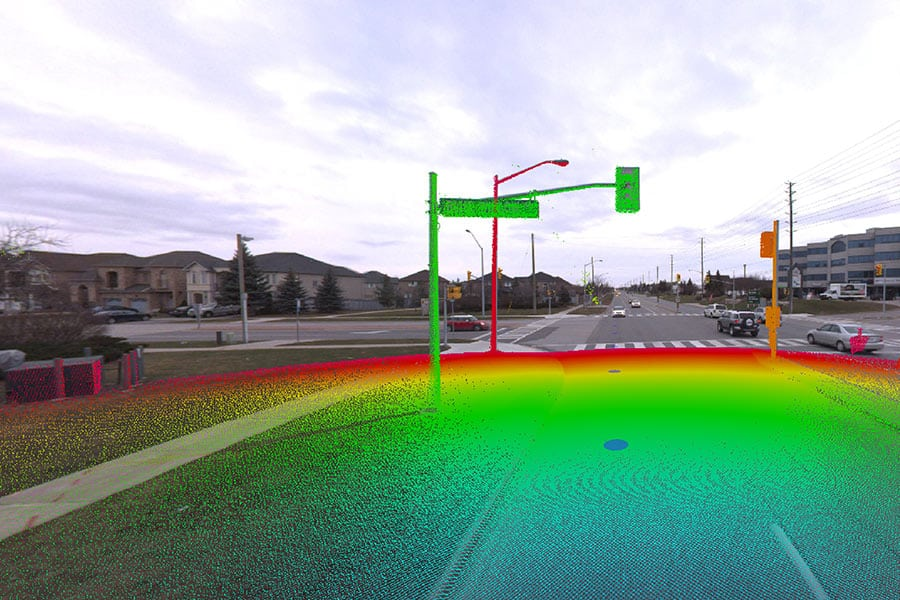
\includegraphics[width=0.6\linewidth]{text_prace/obrazky-figures/Orbit.jpg}
    \caption[Ukážka z~webovej stránky platformy Orbit.]{Ukážka z~webovej stránky platformy Orbit, na ktorej je mračno bodov zobrazené ako vrstva nad záznamom z~kamery. Prevzaté z~\cite{orbit}.}
    \label{fig:orbit}
\end{figure}

Druhou kategóriou sú systémy zamerané na vizualizáciu dát z~autonómnych vozidiel a robotov, ktoré taktiež často zobrazujú mračno bodov, záznam z~kamery a vektorové dáta, ale sú zamerané skôr na zobrazenie dát v~reálnom čase. 

Sem patrí napríklad Autonomous Visualization System (AVS), toolkit pre vývoj webových aplikácií pre vizualizáciu dát z~autonómnych vozidiel, ktorý sa skladá z~dvoch častí: prenosového protokolu XVIZ a toolkitu pre vizualizáciu dát streetscape.gl \cite{avs}. Ukážka aplikácie vytvorenej pomocou toolkitu AVS na webových stránkach tohto projektu je veľmi podobná ukážke na stránkach komerčnej platformy Foxglove, ktorá vizualizuje dáta z~robotov a autonómnych systémov (obr. \ref{fig:foxglove}) \cite{foxglove}. Obe zobrazujú dáta z~autonomného vozidla, ktoré sa skladajú z~neagregovaného mračna bodov, vektorových označení ostatných identifikovaných vozidiel a záznamu z~kamery v~osobitnom okne.

\begin{figure}[h]
    \centering
    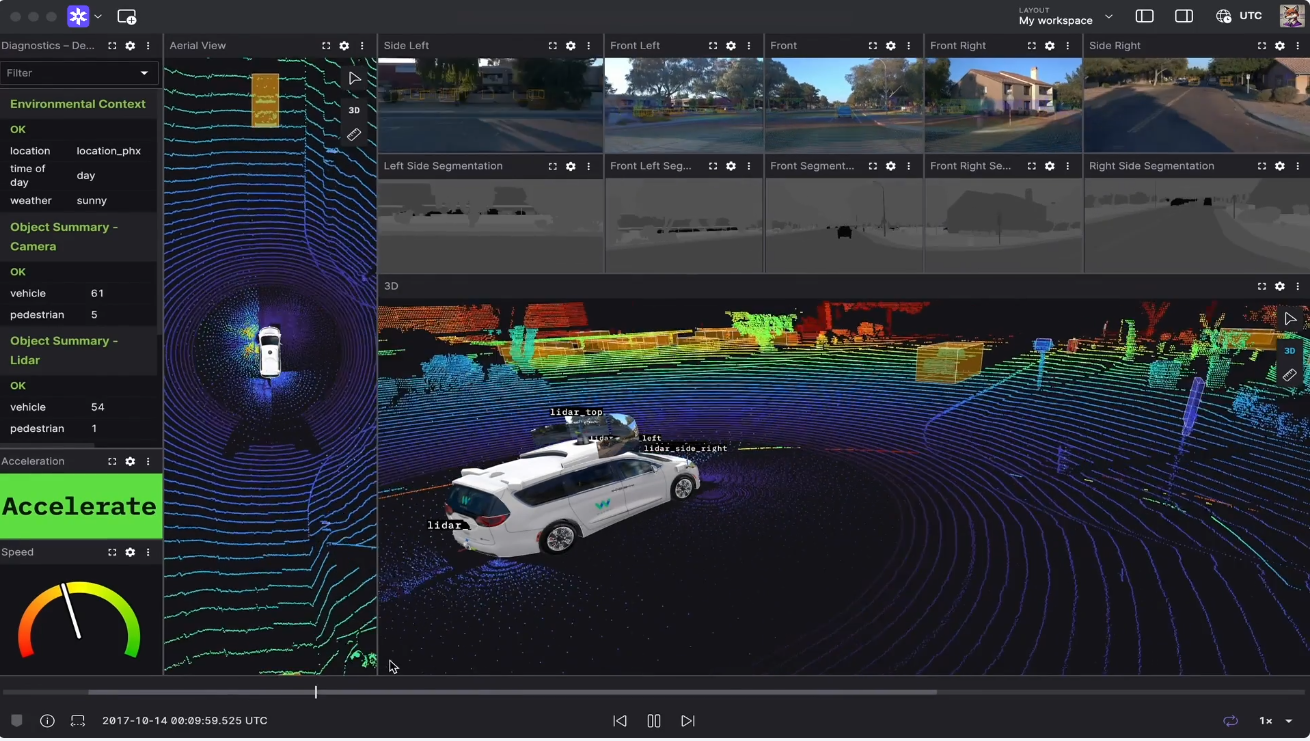
\includegraphics[width=1\linewidth]{text_prace/obrazky-figures/Foxglove.png}
    \caption[Ukážka z~webovej stránky platformy Foxglove.]{Ukážka z~webovej stránky platformy Foxglove, ktorá zobrazuje lidarové a kamerové dáta z~autonómneho automobilu spoločne s~vektorovými dátami. Prevzaté z~\cite{foxglove}.}
    \label{fig:foxglove}
\end{figure}

Okrem toho ešte existuje množstvo komerčných aj voľne dostupných nástrojov, ktoré sú zamerané na zobrazenie a prácu s~mračnami bodov, z~ktorých niektoré dokážu zobraziť aj vektorové dáta, ako napríklad program CloudCompare.

\chapter{Návrh aplikácie}
\label{ch:navrh}

Cieľom tejto práce bolo vytvoriť používateľskú aplikáciu. Výsledná aplikácia mala byť webová, aby ju bolo možné spustiť jednoducho pomocou webového prehliadača. Čo sa týka funkcionality, mala by spĺňať nasledujúce body:

\begin{itemize}
    \item Zobrazenie dát z~mobilného mapovacieho systému. Tieto dáta sú tvorené mračnom bodov z~lidaru, kamerovým záznamom, údajmi o~pohybe vlaku a ďalšími vektorovými dátami a mali by byť zobrazené z~pohľadu strojvedúceho vlaku.
    \item Umožniť používateľovi vybrať si konkrétnu pozíciu vlaku alebo prehrať si animáciu pohybu vlaku s~nastaviteľnou rýchlosťou.
    \item Umožniť používateľovi nahrať súbory s~dátami na zobrazenie: súbor s~mračnom bodov, video z~kamery na čele vlaku, súbor s~vektorovými dátami, textové súbory s~údajmi o~pohybe vlaku -- pole translácií, pole rotácií a pole zodpovedajúcich časových razítok.
    \item Zobrazovať dva typy dát z~lidaru:
    \begin{itemize}
        \item \emph{real-time} -- malé, postupne nasnímané kusy mračna bodov s~časovými razítkami,
        \item \emph{postprocess} -- jedno celistvé mračno bodov, ktoré vzniklo ich spojením.
    \end{itemize}
    (U~oboch typov ide o~agregované dáta -- všetky body sú v~jednej spoločnej súradnicovej sústave). Umožniť používateľovi prepínať medzi týmito dvoma typmi.
    \item Poskytnúť používateľovi možnosti prispôsobenia zobrazenia, ako napríklad zmeny viditeľnosti jednotlivých vrstiev (mračno bodov, vektorové dáta, kamerový záznam) a základné nastavenia zobrazenia mračna bodov (rôzne farebné škály podľa intenzity, veľkosť a priehľadnosť bodov, zobrazenie bodov len do určitej vzdialenosti) aj vektorových dát (farba a hrúbka čiar).
    \item Mať prepínač na zapnutie a vypnutie skreslenia mračna bodov a vektorových dát podľa parametrov skreslenia kamery.
    \item Zobrazovať prejazdný profil vlaku v~predikovanej polohe v~rôznych vzdialenostiach pred vlakom -- 25, 50, 75 a 100m. Zobrazovať aj čiaru spájajúcu predikované polohy. (Súbory s~predikovanými polohami sú súčasťou dát, ktoré aplikácia načítava.)

\end{itemize}

\section{Návrh používateľského rozhrania}

Pri návrhu používateľského rozhrania aplikácie bolo prioritou zobrazenie vizualizácie ako hlavnej časti aplikácie na čo najväčšej ploche a tiež tak, aby bola viditeľná vo všetkých stavoch.

Z~ovládacích prvkov sú za najdôležitejšie považované prvky pre zmenu polohy vlaku, ktoré sú umiestnené v~spodnom paneli. Všetky ostatné ovládacie prvky sú skryté v~bočnom paneli, ktorý sa dá vysunúť tlačítkom v~ľavom hornom rohu, a sú rozdelené do troch záložiek -- nahrávanie dát, prispôsobenie zobrazenia a samostatná záložka pre prejazdný profil. Celkový návrh vzhľadu je na obrázku \ref{fig:navrh_gui}.

\begin{figure}[h]
    \centering
    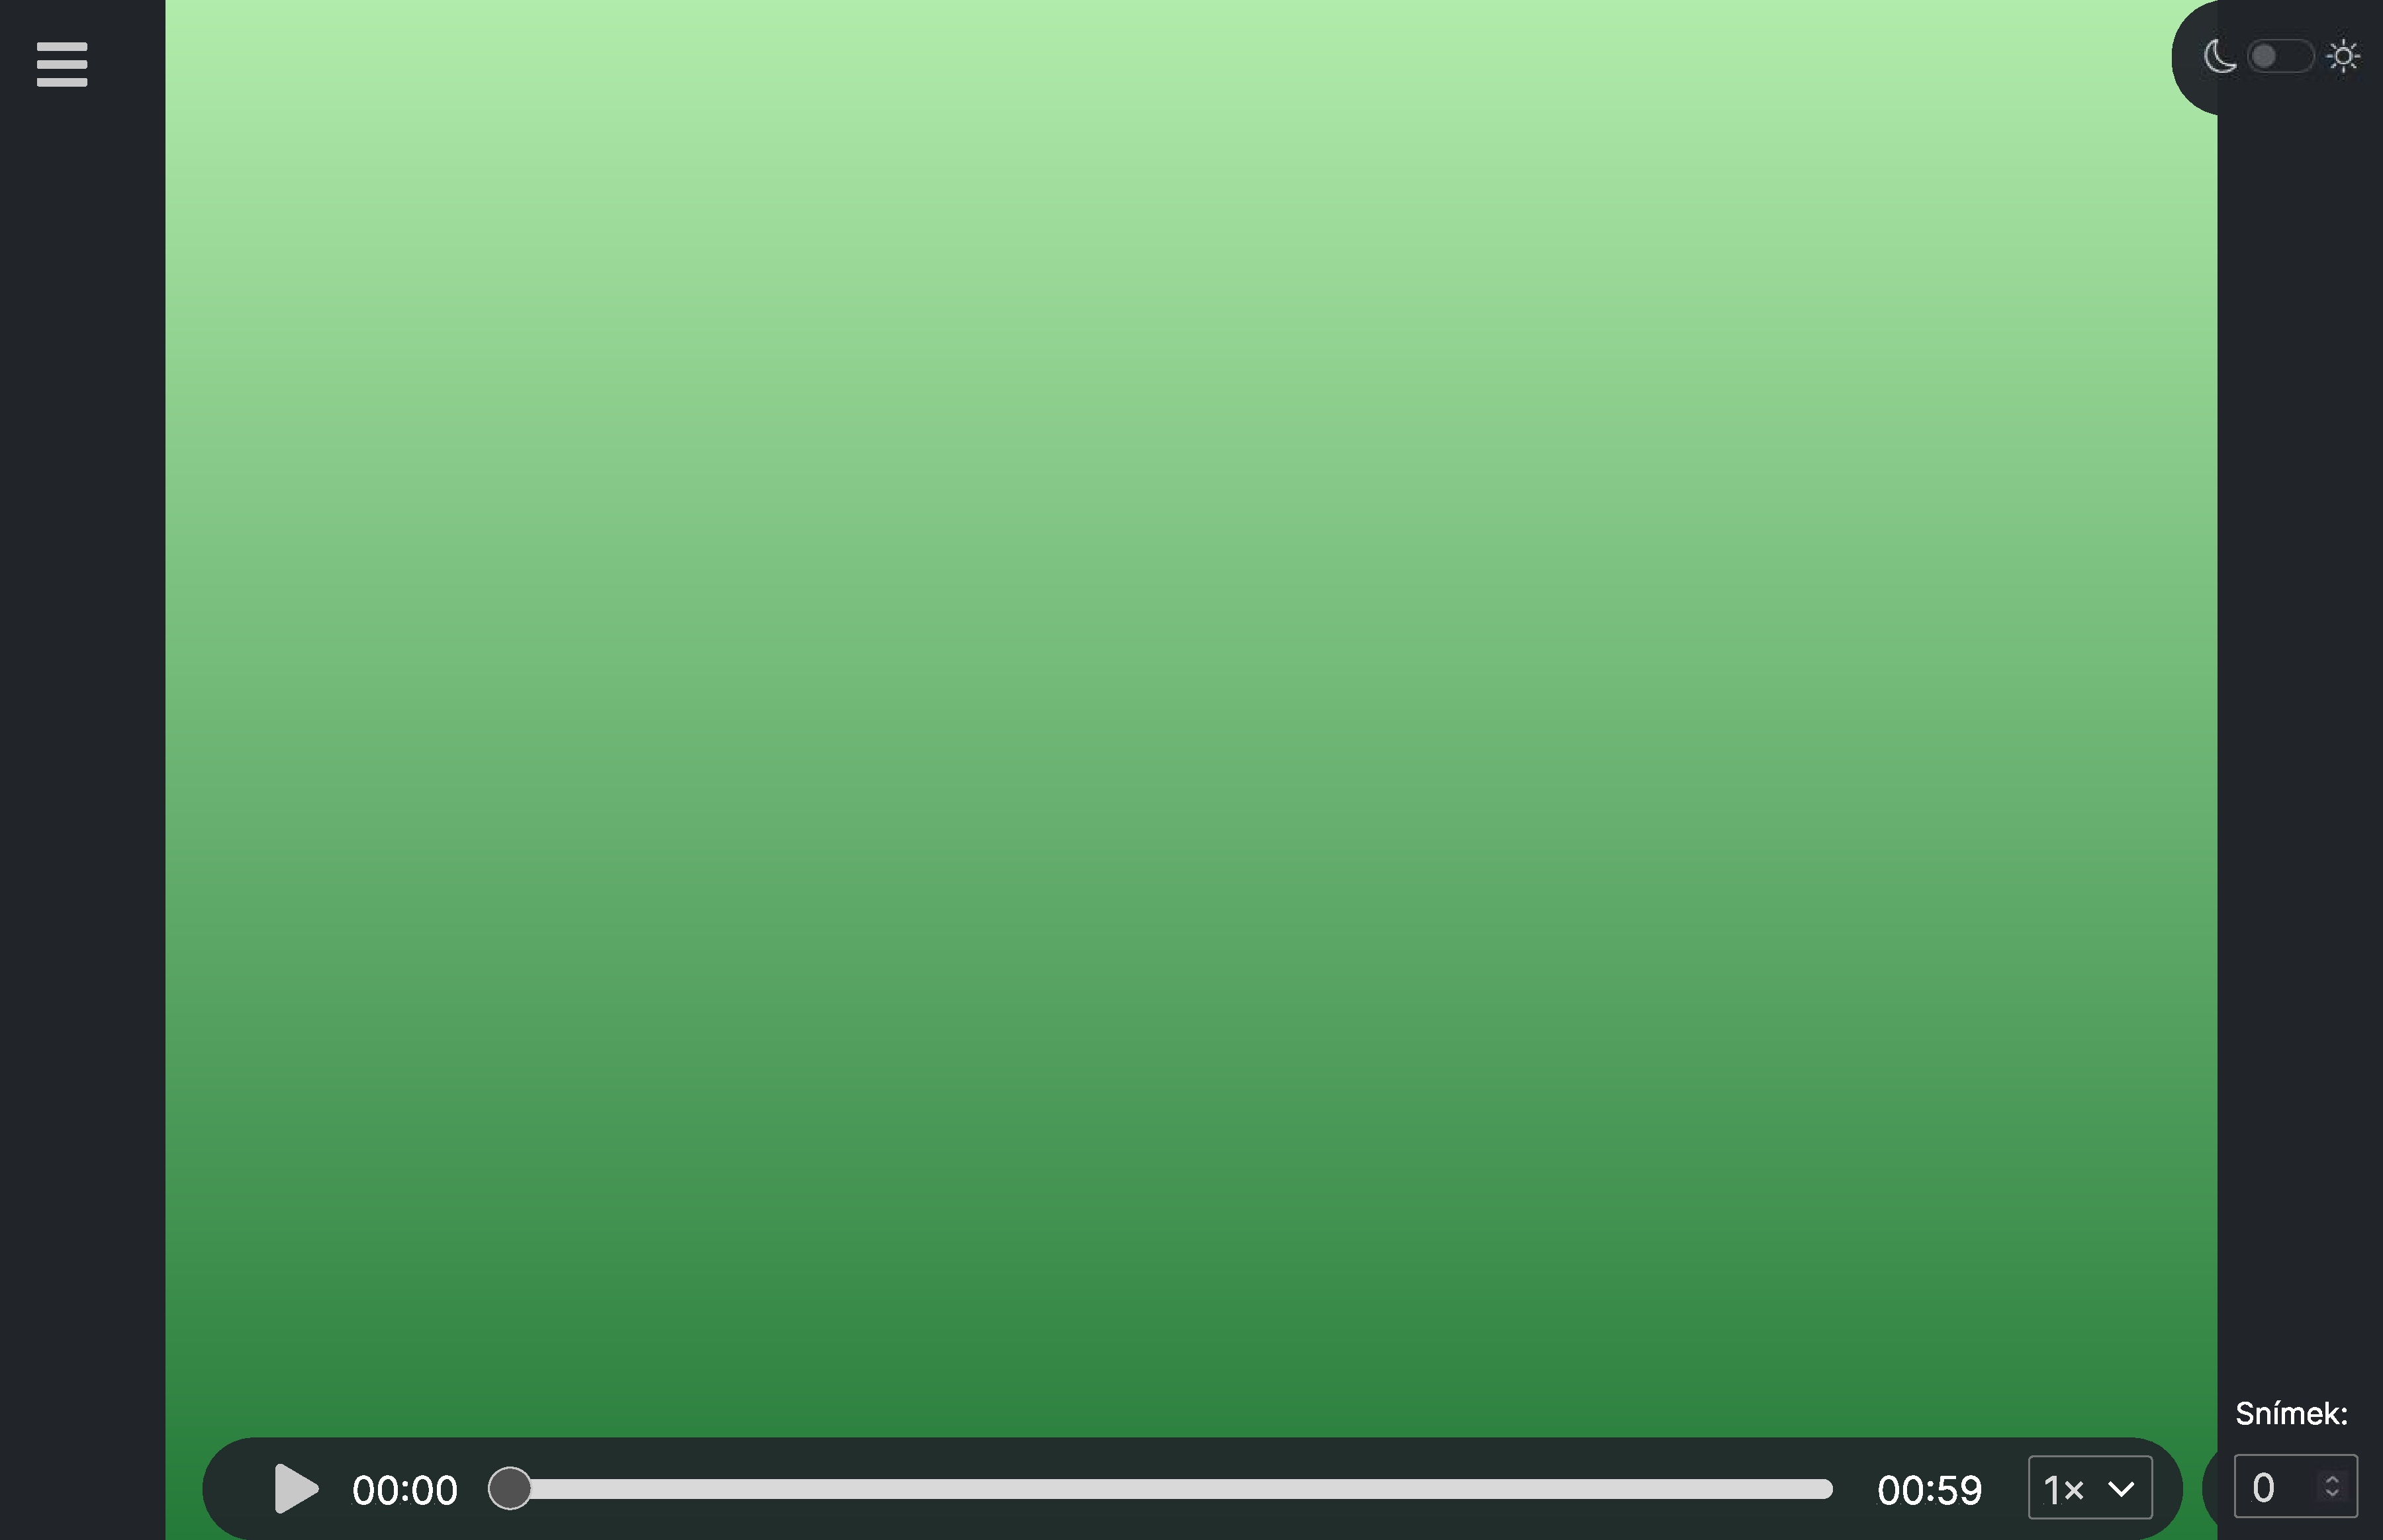
\includegraphics[width=0.9\linewidth]{text_prace/obrazky-figures/navrh1.pdf}
    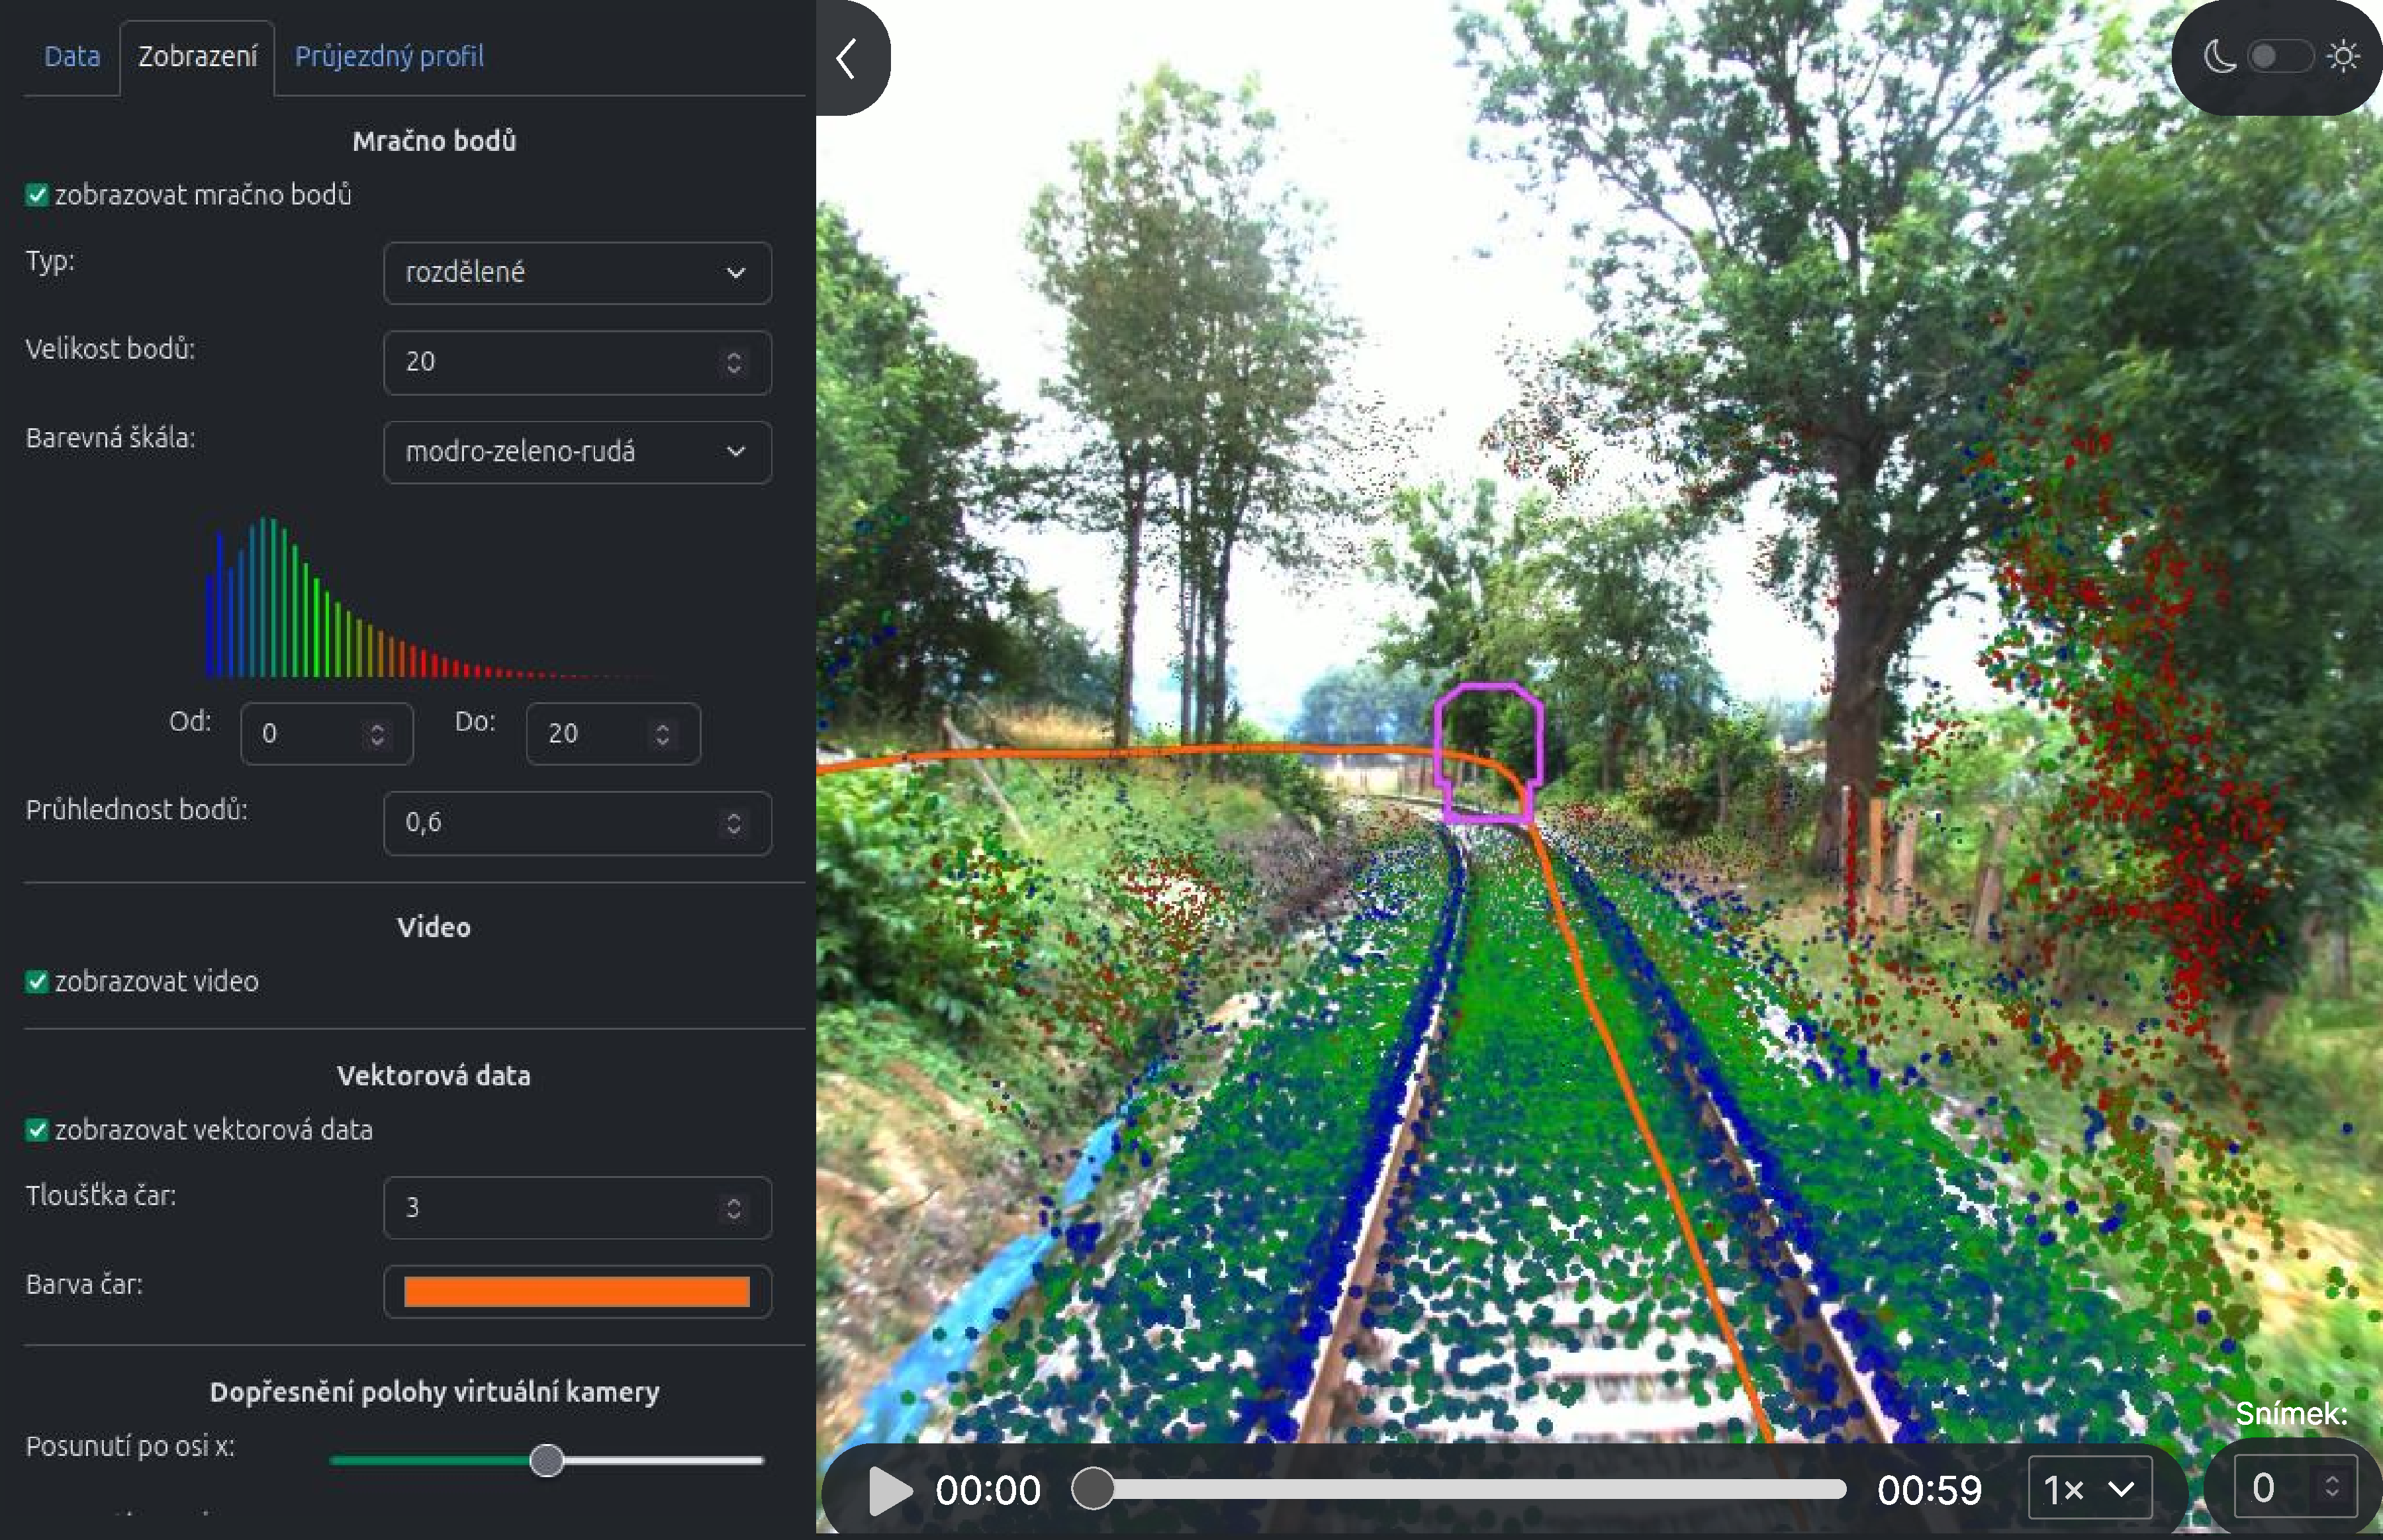
\includegraphics[width=0.9\linewidth]{text_prace/obrazky-figures/navrh2.pdf}
    \caption[Návrh používateľského rozhrania aplikácie.]{Návrh používateľského rozhrania aplikácie vytvorený pomocou nástroja Figma.}
    \label{fig:navrh_gui}
\end{figure}

Hlavnou ideou návrhu je používanie čo najviac štandardných prvkov, aby sa v~aplikácii používatelia ľahko zorientovali. Tomu napomáha aj použitie knižnice Bootstrap, ktorá je u~webových aplikácií veľmi často používaná, a preto budú jej prvky pravdepodobne pre používateľov intuitívne.

Pre používateľskú prívetivosť by mala aplikácia spĺňať nasledujúce body:

\begin{enumerate}
    \item všeobecné vlastnosti:
    \begin{itemize}
        \item intuitívnosť,
        \item responzívny design,
        \item hladký beh animácií,
        \item možnosť exportu a importu nastavení zobrazenia,
        \item svetlý aj tmavý režim,
        \item kompatibilita s~rôznymi prehliadačmi, prípadnú nekompatibilitu používateľovi ohlásiť,
    \end{itemize}
    \item v~záložke \uv{Dáta}:
    \begin{itemize}
        \item prehľadné zobrazenie, aké dáta boli nahrané, možnosť ich nahradenia inými dátami,
        \item zobrazovanie indikátoru, že práve prebieha nahrávanie dát.
    \end{itemize}
\end{enumerate}

\section{Problém nahrávania dát do aplikácie}

Dáta, ktoré má vyvíjaná webová aplikácia zobrazovať, sú rozdelené do väčšieho množstva súborov rôznych typov. Nahrávať ich do aplikácie klasickým spôsobom po jednom či po nejakých skupinách by bolo síce možné, ale pre používateľov časovo náročné a veľmi nepraktické.

Keďže je aplikácia určená úzkej cieľovej skupine používateľov, môžeme si dovoliť predpokladať, že používateľ bude buď spúšťať server webovej aplikácie lokálne, alebo bude mať k~serveru aspoň prístup. Za tohto predpokladu má problém s~nahrávaním dát veľmi elegantné riešenie, a tým je \textbf{projektový súbor}, teda textový súbor, v~ktorom sú špecifikované cesty k~dátovým súborom uloženým na serveri. Používateľovi stačí nahrať tento súbor a aplikácia podľa neho automaticky nahrá všetky potrebné dátové súbory.

Presný formát projektového súboru bolo potrebné navrhnúť. Kompletný návrh je uvedený v~prílohe \ref{ch:project_file}. Bol zvolený formát TOML, ktorý je jednoduchý, praktický a dobre čitateľný \cite{toml}. U~dátových súborov, ktorých môže byť rôzny počet, napríklad súbory s~dátami z~lidaru, sa do projektového súboru uvedie, v~akom priečinku sa nachádzajú, ako sú pomenované a koľko ich je. Predpokladá sa, že sú tieto súbory jednotne pomenované a očíslované (napríklad \texttt{pcd\_0.pcd}, \texttt{pcd\_1.pcd}, \dots).

Keby však bol projektový súbor jediným možným spôsobom nahrávania dát do aplikácie, malo by to isté nevýhody -- napríklad pre vyskúšanie zmeny v~jednom dátovom súbore by bolo potrebné meniť projektový súbor a znova ho nahrávať.

Preto by mala výsledná aplikácia kombinovať oba prístupy, projektový súbor aj klasické nahrávanie dát. Pre jednoduchosť a prístupnosť by mala umožniť nahranie základných súborov klasickým spôsobom. Naopak pre pokročilejšie použitie by mala mať možnosť nahrania projektového súboru, podľa ktorého by mala nahrať všetky špecifikované dátové súbory. Potom by mal používateľ prehľadne vidieť všetky nahrané súbory a mať možnosť tieto súbory jednotlivo ľubovoľne nahradzovať inými súbormi.

\chapter{Implementácia navrhnutej aplikácie}
\label{ch:implementacia}

Navrhnutá webová aplikácia je implementovaná v~jazyku Python s~využitím frameworku Dash. Pre optimalizáciu obsahuje aplikácia aj skript napísaný v~jazyku Javascript, ktorý používa pre vykresľovanie mračna bodov a vektorových dát hardvérovo akcelerovaný framework deck.gl a na rozdiel od zvyšku kódu aplikácie sa vykonáva priamo na klientovi. Táto štruktúra je schematicky znázornená na obrázku \ref{fig:schema_implementacie}. Snímka obrazovky finálnej implementácie je na obrázku \ref{fig:screenshot}.

Vizuálny štýl používateľského rozhrania čiastočne zabezpečuje knižnica Dash Bootstrap Components, čiastočne je dodefinovaný pomocou CSS.

Zdrojový kód je rozdelený do nasledujúcich súborov:
\begin{itemize}
    \item \texttt{app.py} -- Hlavný modul, inicializuje a spustí aplikáciu.
    \item \texttt{params.py} -- Počiatočné parametre.
    \item \texttt{loading\_functions.py} -- Pomocné funkcie pre načítanie dát zo súborov.
    \item \texttt{general\_functions.py} -- Pomocné funkcie pre výpočet projekčnej matice, transformačných matíc a operácií s~rotáciami.
    \item Moduly s~komponentmi a callbackmi rozdelené podľa štruktúry používateľského rozhrania. Sú to štyri dvojice súborov. V~jednom súbore z~dvojice sú vždy definované komponenty používateľského rozhrania vrátane ich vizuálneho štýlu, v~tom druhom k~nim patriace callbacky.
    \item \texttt{visualization.js} -- Vizualizácia mračna bodov a vektorových dát pomocou frameworku deck.gl, riadenie animácie pohybu vlaku. Činnosť tohto skriptu je podrobnejšie popísaná v~sekciách \ref{sec:vrstvy} a \ref{sec:implementacia_animacie}. Pre pripojenie skriptu k~aplikácii tak, aby sa pripojili aj zdrojové kódy frameworku deck.gl, bolo nutné použiť bundler. V~rámci tejto práce bol použitý bundler Webpack. K~aplikácii sa teda nepripája priamo skript \texttt{visualization.js}, ale modul \texttt{bundle.mjs}, ktorý vytvára bundler a sú v~ňom zahrnuté aj zdrojové kódy frameworku deck.gl. Je nutné použiť modul namiesto obyčajného skriptu, pretože mimo modulu nie je v~jazyku JavaScript možné použiť deklaráciu \texttt{import}, ktorá je nutná pre pripojenie zdrojových kódov frameworku deck.gl. 
\end{itemize}

\begin{figure}[t]
    \centering
    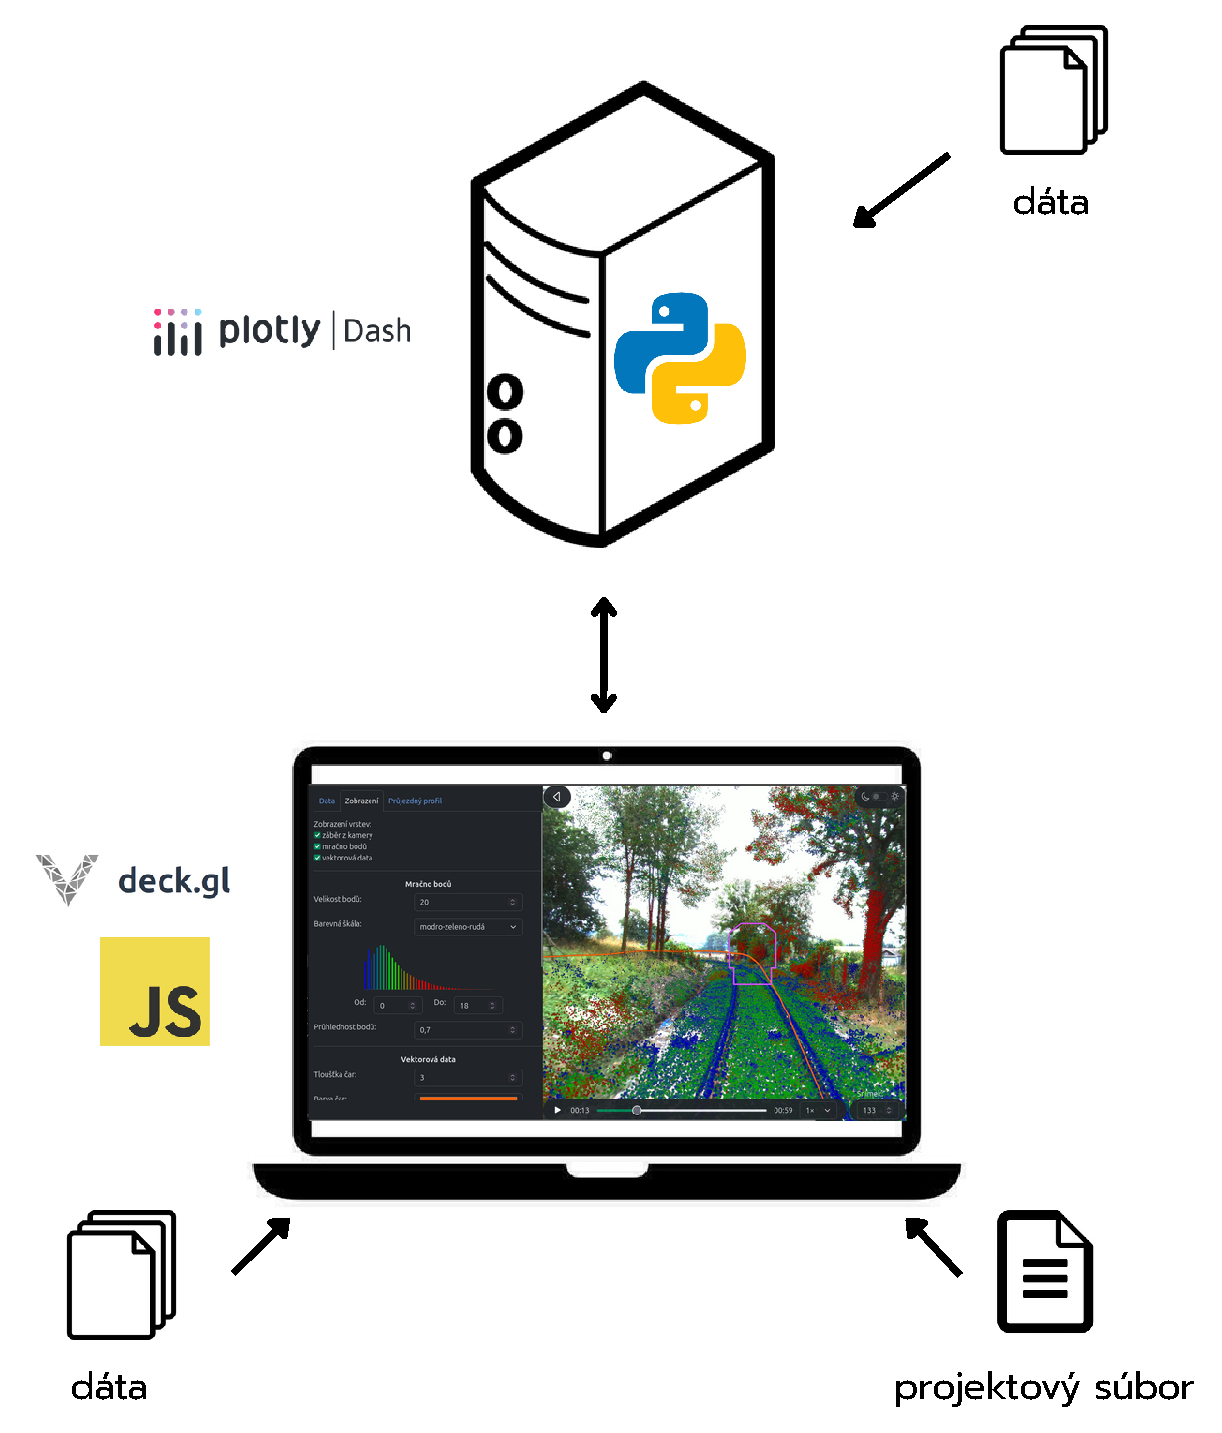
\includegraphics[width=0.7\linewidth]{text_prace/obrazky-figures/schema_implementacie.pdf}
    \caption{Schéma finálnej implementácie.}
    \label{fig:schema_implementacie}
\end{figure}

\begin{figure}[h]
    \centering
    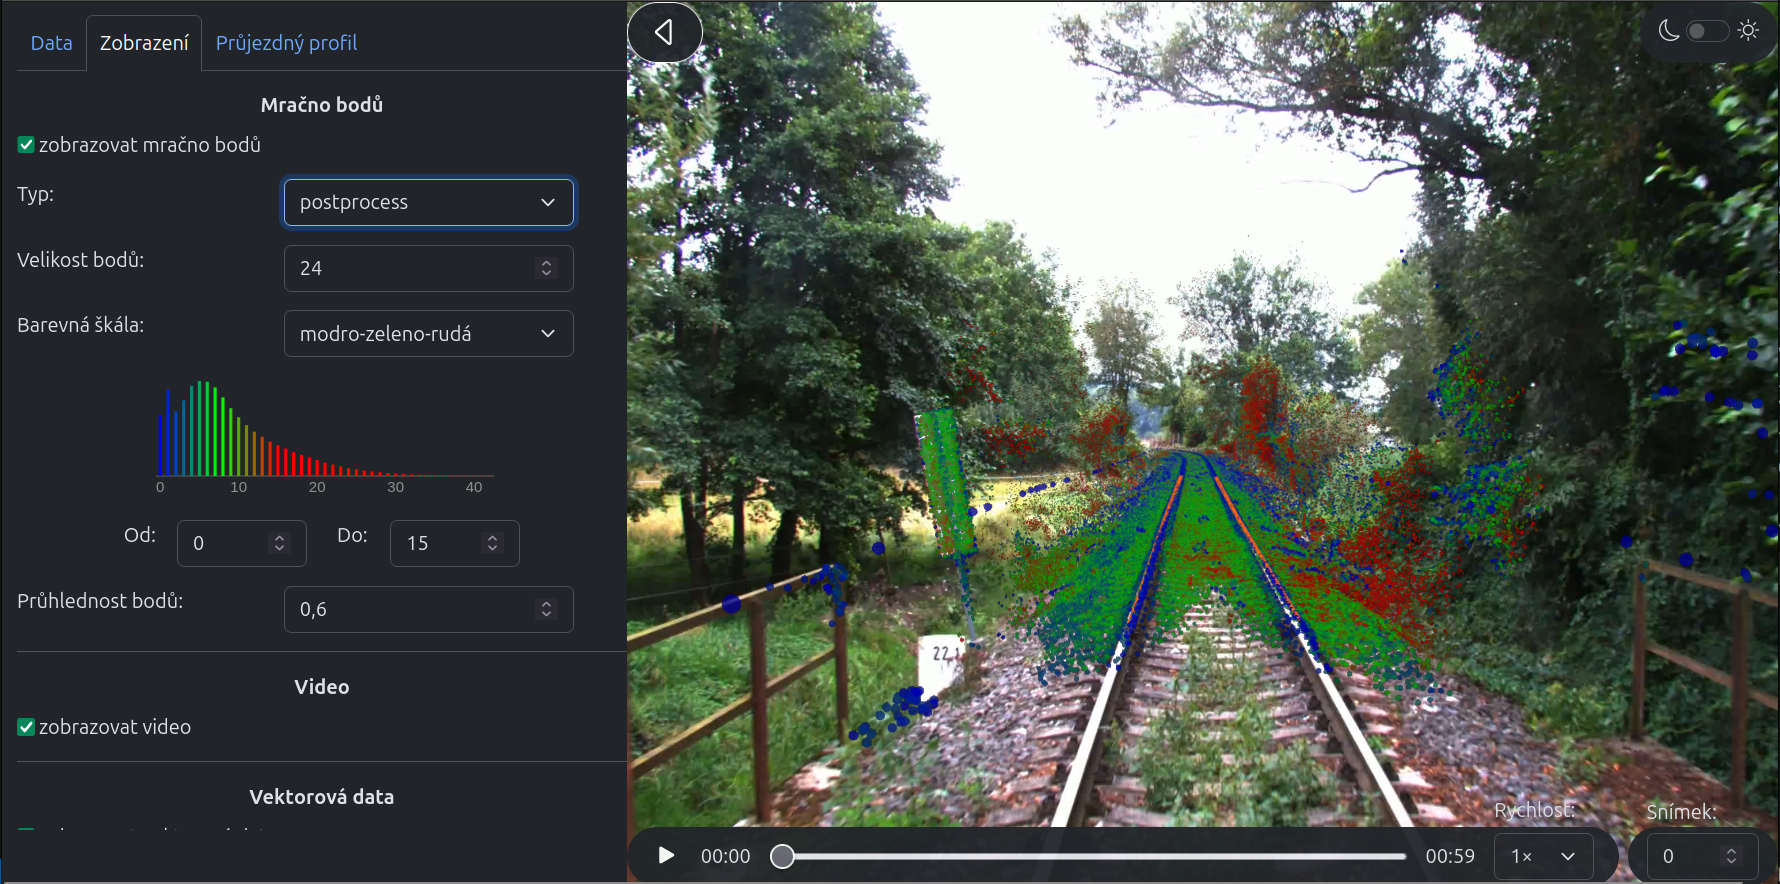
\includegraphics[width=1\linewidth]{text_prace/obrazky-figures/screenshot.png}
    \caption{Snímka obrazovky finálnej implementácie.}
    \label{fig:screenshot}
\end{figure}

\section{Popis modulov}

Táto sekcia sa venuje podrobnejšiemu popisu niektorých modulov.

\subsubsection{Hlavný modul \newline {\normalsize \textmd{(súbor \texttt{app.py})}}}

Načíta zo súborov ukažkové dáta, ktoré aplikácia zobrazí po spustení. Tieto dáta spolu s~počiatočnými parametrami uloží do skladov, z~ktorých ich následne callbacky definované v~module \emph{data} kopírujú do objektu \texttt{window}, aby boli prístupné skriptu \texttt{visualization.js}.

Definuje základné rozloženie a vzhľad aplikácie -- vizualizácia na celú výšku okna, spodný panel, bočný panel s~troma záložkami a prvok na prepínanie svetlého a tmavého režimu. Vizualizácia je zložená z~troch HTML elementov: \texttt{Video}, \texttt{Canvas}, do ktorého vykresľuje dáta framework deck.gl, a druhý \texttt{Canvas} pre implementáciu skreslenia. Toto základné rozloženie je definované väčšinou pomocou CSS pravidiel. Záložka \emph{Data} je obalená komponentom \texttt{Loading} z~knižnice Dash Core Components, ktorý sa používateľovi zobrazuje, keď prebieha aktualizácia niektorého prvku z~tejto záložky, teda keď aplikácia nahráva dáta.

Modul načíta všetky potrebné komponenty a callbacky z~iných modulov, inicializuje a spustí aplikáciu. Obsahuje tri klientske callbacky -- jeden pre inicializáciu vizualizácie, jeden pre vysúvanie bočného panelu a jeden pre prepínanie svetlého a tmavého režimu.

\subsubsection{Modul \emph{animation control} \newline {\normalsize \textmd{
(súbory \texttt{animation\_control\_components.py}, \texttt{animation\_control\_callbacks.py})
}}}

Obsahuje prvky pre ovládanie animácie -- spustenie a zastavenie, posunutie, zmena rýchlosti, výber konkrétneho snímku, -- ktoré sa nachádzajú v~spodnom paneli. Prvky sú rozmiestnené s~využitím CSS mechanizmov \emph{grid} a \emph{flexbox}.

Keďže riadenie animácie prebieha na strane klienta, všetky callbacky v~tomto module sú klientske a väčšinou volajú funkcie definované v~skripte \texttt{visualization.js}. Mechanizmus riadenia animácie je popísaný v~sekcii \ref{sec:implementacia_animacie}.

Zmena rýchlosti animácie prebieha tak, že sa u~videa zmení vlastnosť \texttt{playbackRate}. Tým sa zmení rýchlosť videa, a keďže vykresľovanie mračna bodov a vektorových dát je naviazané na video, zrýchli sa tým celá animácia.

\subsubsection{Modul \emph{data} \newline {\normalsize \textmd{
(súbory \texttt{data\_tab\_components.py}, \texttt{data\_tab\_callbacks.py})
}}}

Tvorí záložku \emph{Data} v~bočnom paneli a riadi nahrávanie dát do aplikácie. Obsahuje komponenty dvoch typov -- \texttt{*\_upload} a \texttt{*\_uploaded\_file[s]}. Komponenty typu \texttt{*\_upload} umožňujú manuálne nahranie súborov do aplikácie. Keď také nahranie prebehne, komponent \texttt{*\_upload} je skrytý a namiesto neho sa zobrazí komponent \texttt{*\_uploaded\_file[s]}, ktorý používateľovi pre kontrolu zobrazuje názov nahraného súboru a obsahuje aj tlačítko v~tvare~x, ktoré skryje komponent \texttt{*\_uploaded\_file[s]} a znova zobrazí komponent \texttt{*\_upload}, čím umožní používateľovi nahrať iný súbor.

Špeciálnym typom nahrávaného súboru je projektový súbor, ktorý vyvolá automatické nahranie všetkých v~ňom definovaných súborov.

Niektoré typy dát nemajú komponent \texttt{*\_upload} a dajú sa nahrať iba pomocou projektového súboru. Sú to tie typy dát, ktoré sa skladajú z~viacerých súborov, a to konkrétne mračno bodov typu real-time, vektorové dáta a polohy prejazdného profilu.

Väčšina callbackov je napísaná v~Pythone, spracúvajú nahrané súbory a spracované dáta ukladajú do skladov (komponenty \texttt{Store}).

Isté špecifiká sú u~nahrávania súboru s~mračnom bodov a videa. Framework Dash totiž načítané súbory odovzdáva callbackom ako pole bytov, ale použitá knižnica \texttt{pypcd4} dokáže načítať súbor vo formáte \texttt{pcd} iba podľa cesty k~súboru. Preto je nahraný súbor s~mračnom bodov uložený ako dočasný súbor do priečinka \texttt{assets/temp}, odtiaľ nahraný a potom hneď zmazaný.

Podobne je to u~videa, ktoré je tiež potrebné uložiť ako dočasný súbor a potom nastaviť cestu k~nemu do atribútu \texttt{src} komponentu \texttt{html.Video}. Na rozdiel od súboru s~mračnom bodov ho však nie je možné zmazať hneď v~tom istom callbacku, musí v~priečinku \texttt{assets/temp} po istú dobu zostať, pretože jeho nahranie do aplikácie nejakú dobu trvá. Preto je definovaný špeciálny callback, ktorý sa spustí každé dve minúty a vymaže všetky dočasné súbory staršie než dve minúty. Okrem toho novému videu po nahraní musí byť nastavený rovnaký čas, ako malo to predchádzajúce, čo je zabezpečené ďalším callbackom.

Ďalej sú v~tomto module ešte klientske callbacky, ktoré kopírujú nové dáta zo skladov do objektu \texttt{window}, aby boli prístupné skriptu \texttt{visualization.js}.

\subsubsection{Modul \emph{visualization} \newline {\normalsize \textmd{
(súbory \texttt{visualization\_tab\_components.py}, \texttt{visualization\_tab\_callbacks.py})
}}}

Tvorí záložku \emph{Zobrazení} v~bočnom paneli a obsahuje všeobecné nastavenia týkajúce sa zobrazenia. Dôležitou funkciou je voľba typu zobrazovaného mračna bodov -- postprocess alebo real-time.

Najzložitejším komponentom je graf, ktorý zobrazuje rozloženie bodov podľa intenzity a zároveň aj farebnú škálu (ukážka je na obrázku \ref{fig:farebna_skala}). Ďalej táto záložka obsahuje aj posuvníky pre upresnenie polohy kamery a tlačidlá pre export a import nastavení zobrazenia. Nastavenia sa exportujú vo formáte \texttt{toml}. Táto možnosť je užitočná najmä pre uloženie nastavenia posuvníkov, ale ukladá aj všetky ostatné nastavenia zo záložiek \emph{Zobrazení} a \emph{Průjezdný profil}.

Nachádza sa tu aj možnosť zapnutia a vypnutia skreslenia vizualizácie podľa parametrov skreslenia kamery.

Modul obsahuje niekoľko klientskych callbackov, ktoré volajú funkcie definované v~skripte \texttt{visualization.js}.

Ďalej je tu viacero callbackov patriacich ku grafu zobrazujúcemu farebnú škálu. Keďže je to zložitý komponent, obsahuje štyri sklady, do ktorých sa ukladá typ farebnej škály, jej rozsah a agregácia mračna bodov oboch typov, ktoré aplikácia zobrazuje. Graf sa aktualizuje, keď sa zmení ktorýkoľvek z~týchto údajov, alebo keď sa zmení typ zobrazovaného mračna bodov.

V~module sa ešte nachádzajú callbacky pre počítanie skreslenia, ktoré sú bližšie popísané v~sekcii \ref{sec:implementacia_skreslenia}.

\subsubsection{Modul \emph{profile} \newline {\normalsize \textmd{
(súbory \texttt{profile\_tab\_components.py}, \texttt{profile\_tab\_callbacks.py})
}}}

Tvorí záložku \emph{Průjezdný profil} v~bočnom paneli a obsahuje iba nastavenia týkajúce sa zobrazenia prejazdného profilu a čiary cez polohy prejazdného profilu. Umožnuje používateľovi vybrať si, ktorú predikciu chce vidieť -- na 25, 50, 75 alebo 100 metrov.

Callbacky sú klientske a volajú funkcie definované v~skripte \texttt{visualization.js}.

\section{Rozdelenie dát do vrstiev}
\label{sec:vrstvy}

Pri vizualizácii dát pomocou frameworku deck.gl sú použité dva typy vrstiev:
\begin{itemize}
    \item \texttt{PointCloudLayer} pre mračno bodov,
    \item \texttt{PathLayer} pre vektorové dáta.
\end{itemize}
Rozdelenie vizualizácie na vrstvy je znázornené na obrázku \ref{fig:vrstvy}.

\begin{figure}[h]
    \centering
    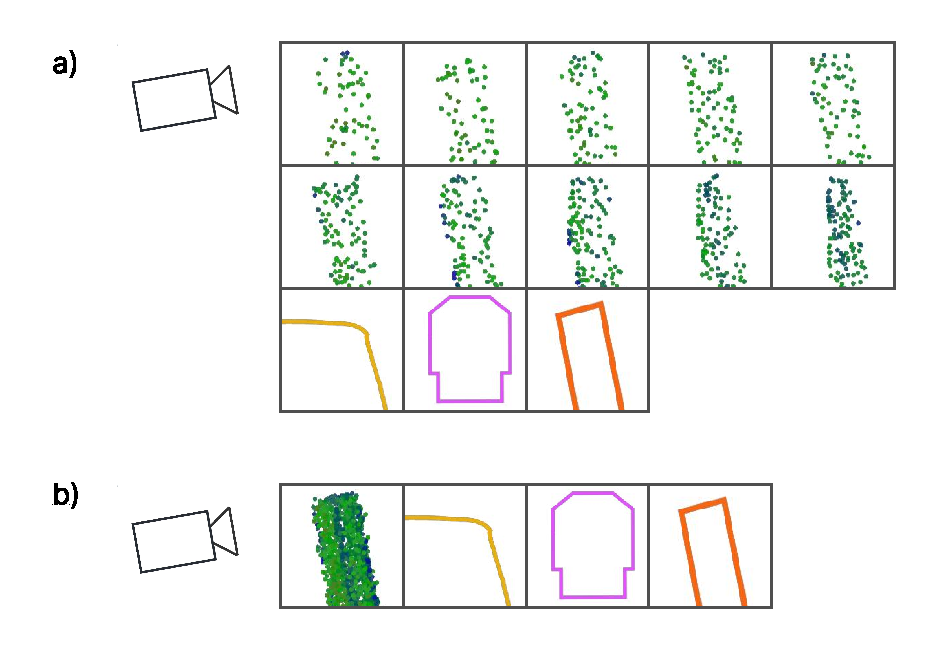
\includegraphics[width=0.8\linewidth]{text_prace/obrazky-figures/vrstvy.pdf}
    \caption[Schéma rozdelenia dát do vrstiev.]{Schéma rozdelenia dát do vrstiev. Počet vrstiev s~mračnom bodov závisí od typu zobrazovaného mračna bodov.}
    \label{fig:vrstvy}
\end{figure}

Na začiatku tvorby práce bola na zobrazenie vektorových dát použitá vrstva \texttt{LineLayer}. Ukázalo sa však, že vstva \texttt{LineLayer} je prispôsobená iba pre zobrazovanie čiar na mapách a pri použití nemapového pohľadu ako \texttt{FirstPersonView} nefunguje dobre -- niektoré čiary sa otáčajú kolmo ku kamere a tým pádom sa ich šírka zmenšuje, niekedy až tak, že úplne prestanú byť viditeľné. Toto správanie u~vrstvy \texttt{LineLayer} nie je možné zmeniť. Naopak u~vrstvy \texttt{PathLayer} je možné nastaviť vlastnosť \texttt{billboard}, ktorá znamená otočenie čiar smerom ku kamere, preto bola nakoniec táto vrstva použitá namiesto vrstvy \texttt{LineLayer}. \texttt{PathLayer} sa od \texttt{LineLayer} líši ešte tým, že čiary majú pevnú šírku v~pixeloch a nezužujú sa podľa toho, ako ďaleko sú od kamery.

Vizualizácia obsahuje nasledujúce vrstvy:
\begin{itemize}
    \item Mračno bodov. Ak aplikácia zobrazuje mračno bodov typu real-time, teda malé, postupne nasnímané časti s~časovými razítkami, tak je vrstiev desať a zobrazujú desať z~týchto častí -- jednu, ktorá zodpovedá danej pozícii, a deväť predchádzajúcich (obrázok \ref{fig:vrstvy}, časť a)). Ak aplikácia zobrazuje mračno bodov typu postprocess, tak je celé v~jednej vrstve (obrázok \ref{fig:vrstvy}, časť b)).
    \item Čiara spájajúca predikované polohy prejazdného profilu vlaku.
    \item Prejazdný profil vlaku v~predikovanej polohe. Od ostatných vektorových dát sa líši tým, že sa jeho poloha mení pri zmene polohy kamery. To je v~implementácii dosiahnuté pomocou špeciálnej prístupovej funkcie \texttt{profileGetPath} (prístupové funkcie boli popísané v~sekcii \ref{sec:nastavenie_polohy_kamery}, podsekcia Aplikovanie transformácií na dáta). 
    \item Ďalšie vektorové dáta.
\end{itemize}

\subsubsection{Farebné škály}

Okrem polohy má každý bod v~mračne bodov v~dodanej sade dát určenú ešte jednu vlastnosť -- intenzitu v~rozmedzí od 0 do 42, ktorú je vhodné farebne rozlíšiť.

Boli implementované dve farebné škály, klasická modro-zeleno-červená a žlto-fialová, pričom u~oboch si môže používateľ zvoliť, od akej intenzity začína a pri akej končí. Ak je napríklad nastavená žlto-fialová farebná škála od 0 do 20, tak to znamená, že body s~intenzitou 0 budú mať žltú farbu, body s~intenzitou 20 a vyššou fialovú farbu a body s~intenzitou od 1 do 19 kombinovanú farbu.

Pre prehľadnosť bol tiež implementovaný graf, ktorý používateľovi ukazuje relatívne počty bodov s~jednotlivými intenzitami a aké majú nastavené farby. Ukážky možných nastavení sú na obrázku \ref{fig:farebna_skala}.

\begin{figure}[h]
    \centering
    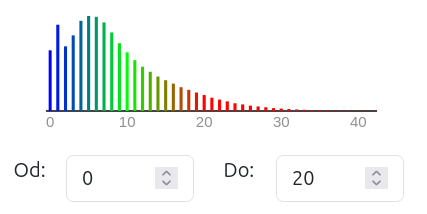
\includegraphics[width=0.35\linewidth]{text_prace/obrazky-figures/farebna_skala1.png}
    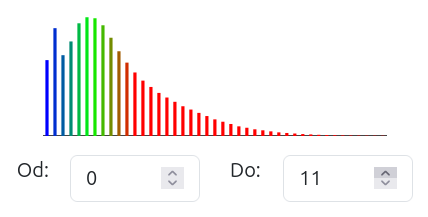
\includegraphics[width=0.35\linewidth]{text_prace/obrazky-figures/farebna_skala2.png}
    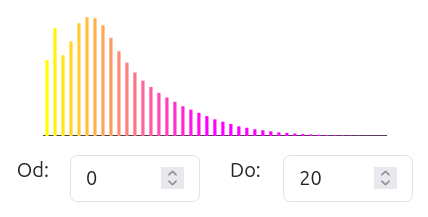
\includegraphics[width=0.35\linewidth]{text_prace/obrazky-figures/farebna_skala3.png}
    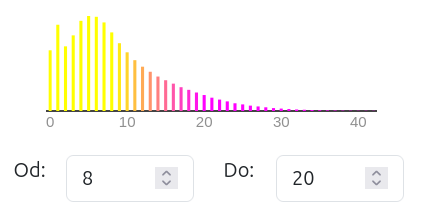
\includegraphics[width=0.35\linewidth]{text_prace/obrazky-figures/farebna_skala4.png}
    \caption[Nastaviteľná farebná škála pre mračno bodov.]{Nastaviteľná farebná škála pre mračno bodov. Vodorovná os predstavuje intenzitu, vertikálna os predstavuje počet bodov.}
    \label{fig:farebna_skala}
\end{figure}

\section{Implementácia animácie pohybu vlaku}
\label{sec:implementacia_animacie}

Animácia pohybu vlaku sa vykonáva výhradne na strane klienta, bez komunikácie so serverom. Zabezpečujú ju tri javascriptové funkcie, ktorých definícia sa nachádza v~súbore \texttt{visualization.js}: \texttt{runDeckAnimation}, \texttt{stopDeckAnimation} a \texttt{animationStep}.

V~tejto sekcii je popísaný princíp fungovania animácie, pre prehľadnosť boli vynechané niektoré menej dôležité implementačné detaily.

Keď používateľ klikne na tlačítko pre prehranie animácie, spustí sa klientsky callback, ktorý vykoná nasledujúci kód:

\begin{lstlisting}
const video = document.getElementById('background-video');
window.runDeckAnimation();
video.play();
video.onpause = function(){ window.stopDeckAnimation() };
\end{lstlisting}

Funkcia \texttt{runDeckAnimation} reinicializuje niektoré parametre, ak je to potrebné, a potom zavolá funkciu \texttt{animationStep}.

Funkcia \texttt{animationStep} vykonáva tieto kroky:

\begin{enumerate}
    \item Najprv zabezpečí, aby sa zavolala znova pri najbližšom vykreslení nového snímku vo videu:
    \begin{lstlisting}
const video = document.getElementById('background-video');
video.requestVideoFrameCallback(animationStep);
    \end{lstlisting}

    \item Potom na základe časových razítok polôh kamery v~mračne bodov a aktuálneho času videa vypočíta aktualizovanú polohu kamery. Ak je to posledná poloha, zastaví video metódou \texttt{pause}.

    \item Ak aplikácia zobrazuje mračno bodov typu real-time, tak následne na základe časových razítok mračna bodov zistí, či by sa nemali zobraziť nejaké nové časti. Vymieňanie častí prebieha efektívnym cyklickým spôsobom, ktorý je znázornený na obrázku \ref{fig:vrstvy_animacia}.

    \item Potom prebehne samotná aktualizácia vizualizácie (v~skripte funkcia \texttt{updateDeck}), kedy sa kamera posunie na novú polohu a aktualizujú sa vrstvy (v~skripte funkcia \texttt{createLayers}), čím sa posunie prejazdný profil a prípadne sa vymenia časti mračna bodov.

    \item Ako posledné sa aktualizujú prvky v~grafickom používateľskom rozhraní, ktoré ukazujú stav animácie -- posuvník, čas a vstupné pole s~číslom snímky.
\end{enumerate}

\begin{figure}[t]
    \centering
    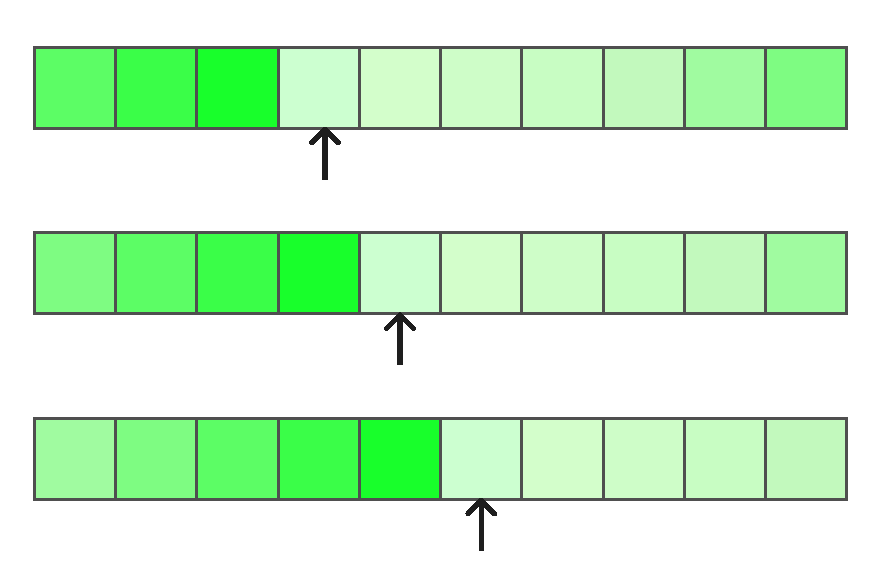
\includegraphics[width=0.4\linewidth]{text_prace/obrazky-figures/vrstvy_animacia.pdf}
    \caption[Schéma cyklického prepisovania deck.gl vrstiev obsahujúcich mračno bodov typu real-time.]{Schéma cyklického prepisovania deck.gl vrstiev obsahujúcich mračno bodov typu real-time. Vizualizácia obsahuje vždy desať vrstiev, ktoré zobrazujú desať častí mračna bodov. Ak podľa časových razítok má byť zobrazená nejaká nová časť, tak sa prepíše vždy tá najstaršia.}
    \label{fig:vrstvy_animacia}
\end{figure}

Animácia sa končí buď tak, že používateľ klikne na tlačítko pre zastavenie animácie, čím sa spustí klientsky callback, ktorý zastaví video metódou \texttt{pause}, alebo tak, že skončí video, alebo tak, že je dosiahnutá posledná poloha kamery. V~každom prípade sa spustí funkcia \texttt{stopDeckAnimation}, pretože bola na začiatku animácie nastavená ako callback pre udalosť zastavenia videa.

Funkcia \texttt{stopDeckAnimation} upovedomí framework Dash o~novej hodnote posuvníka, času a vstupného poľa s~číslom snímku. Toto sa nevykonáva počas animácie, pretože je to výkonovo náročné.

\section{Implementácia skreslenia}
\label{sec:implementacia_skreslenia}

Pri zobrazovaní mračna bodov a vektorových dát tak, aby zobrazenie čo najpresnejšie sedelo na záznam z~kamery, je potrebné vziať do úvahy aj skreslenie kamery, ktoré bolo popísané v~sekcii \ref{sec:skreslenie}. 

Parametre skreslenia boli súčasťou dodaných dát. Existuje niekoľko možností, ako ich použiť:
\begin{enumerate}
    \item Odstrániť skreslenie zo záznamu z~kamery.
    \item Aplikovať skreslenie na mračno bodov, a to:
    \begin{enumerate}
        \item meniť súradnice bodov v~rámci niektorej transformácie vo vykresľovacom reťazci,
        \item aplikovať skreslenie až na finálny obraz.
    \end{enumerate}
\end{enumerate}

Možnosti 1 a 2b) sú výkonovo približne rovnako náročné a výkonnosť závisí od rozmerov vizualizácie v~pixeloch.

Možnosť 2a) by bola v~rámci frameworku realizovateľná dvoma spôsobmi: buď výpočtom skreslenia v~prístupových funkciách, alebo implementáciou vlastných vrstiev a napísaním vlastného kódu pre vertex shader. Akékoľvek výpočty v~prístupových funkciách však majú výrazný vplyv na výkon, výpočet skreslenia je pomerne zložitý (oproti napríklad násobeniu maticou, ktoré sa u~bežných transformácii používa) a výkonnosť by sa naviac zhoršovala s~počtom vykresľovaných bodov. Druhý spôsob je implementačne náročný a realizácia by zabrala veľa času.

Preto bola zvolená a implementovaná možnosť 2b).

Pri hľadaní existujúcich riešenení podobných problémov bol nájdený článok od J. Balocha, ktorý sa zaoberá aplikáciou rôznych efektov na obrázky vo webových stránkach pomocou Javascriptu \cite{baloch_distortion_in_js}.

Toto riešenie funguje tak, že vytvorí element \texttt{Canvas} rovnakej veľkosti ako pôvodný obrázok, cyklom prechádza všetky pixely obrázku a pre každý pixel vypočíta jeho novú polohu a vykreslí ho do elementu \texttt{Canvas}.

Myšlienka tohto riešenia bola využitá aj pri implementácii skreslenia v~tejto práci, ale s~niekoľkými rozdielmi.

Poprvé, pixely sa nečítajú z~obrázku, ale z~elementu \texttt{Canvas}, do ktorého vykresľuje zobrazenie framework deck.gl. Keďže je tento element naviazaný na framework deck.gl, nie je možné z~neho prečítať pixel jednoducho príkazmi 

\begin{lstlisting}
ctx = canvas.getContext("2d");
pixelData = ctx.getImageData(...);
\end{lstlisting}

Namiesto toho je nutné použiť rozhranie WebGL:

\begin{lstlisting}
const gl_ctx = canvas.getContext("webgl2");
const pixelData = new Uint8Array(width * height * 4);
gl_ctx.readPixels(0, 0, width, height, gl_ctx.RGBA, gl_ctx.UNSIGNED_BYTE, 
    pixelData);
\end{lstlisting}

Podruhé, keďže vo vyvíjanej aplikácii je potrebné počítať skreslenie mnohokrát s~tými istými parametrami a rozmermi obrazu, bolo by neefektívne pri každom výpočte počítať novú polohu pre každý pixel, pretože tieto hodnoty sa nemenia.

Preto je skreslenie implementované dvoma klientskymi callbackmi. Ten prvý vypočíta pre každý pixel jeho novú polohu v~skreslenom obraze a výsledky uloží do poľa v~objekte \texttt{window}. Tento výpočet je nutné zopakovať iba vtedy, keď sa zmenia rozmery vizualizácie. Ten druhý reaguje na vypnutie a zapnutie skreslenia používateľom. Keď je skreslenie zapnuté, skryje element \texttt{visualization-canvas}, do ktorého vykresľuje zobrazenie deck.gl, zviditeľní namiesto neho element \texttt{distorted-visualization-canvas}, ktorý má rovnakú veľkosť a pozíciu, a zaregistruje javascriptový callback, ktorý po každom vykreslení zobrazenia frameworkom deck.gl prečíta hodnotu všetkých pixelov a prekreslí ich na predpočítané pozície do elementu \texttt{distorted-visualization-canvas}.

\chapter{Testovanie a evaluácia}
\label{ch:vyhodnotenie}

Pri vývoji aplikácie bola k~dispozícii iba jedna sada dát, ktorú bolo možné použiť pre testovanie.

Už pri prvých pokusoch o~zobrazenie mračna bodov sa ukázalo, že údaje o~polohách kamery sú v~inom súradnicovom systéme ako mračno bodov, pretože sa líši poradie ôs, čomu bola implementácia prispôsobená.

Ďalej sa ukázalo, že aj pri zobrazení mračna bodov presne podľa dodanej polohy kamery a kalibračnej matice zobrazenie nesedí presne na záznam z~kamery a je potrebné pridať isté posunutie a rotáciu. Preto boli do používateľského rozhrania aplikácie pridané posuvníky, ktorými si používateľ môže prispôsobiť polohu virtuálnej kamery (posunutím a otočením v~istom rozsahu), a tým opraviť nepresnosti v~dátach.

\begin{figure}[h]
    \centering
    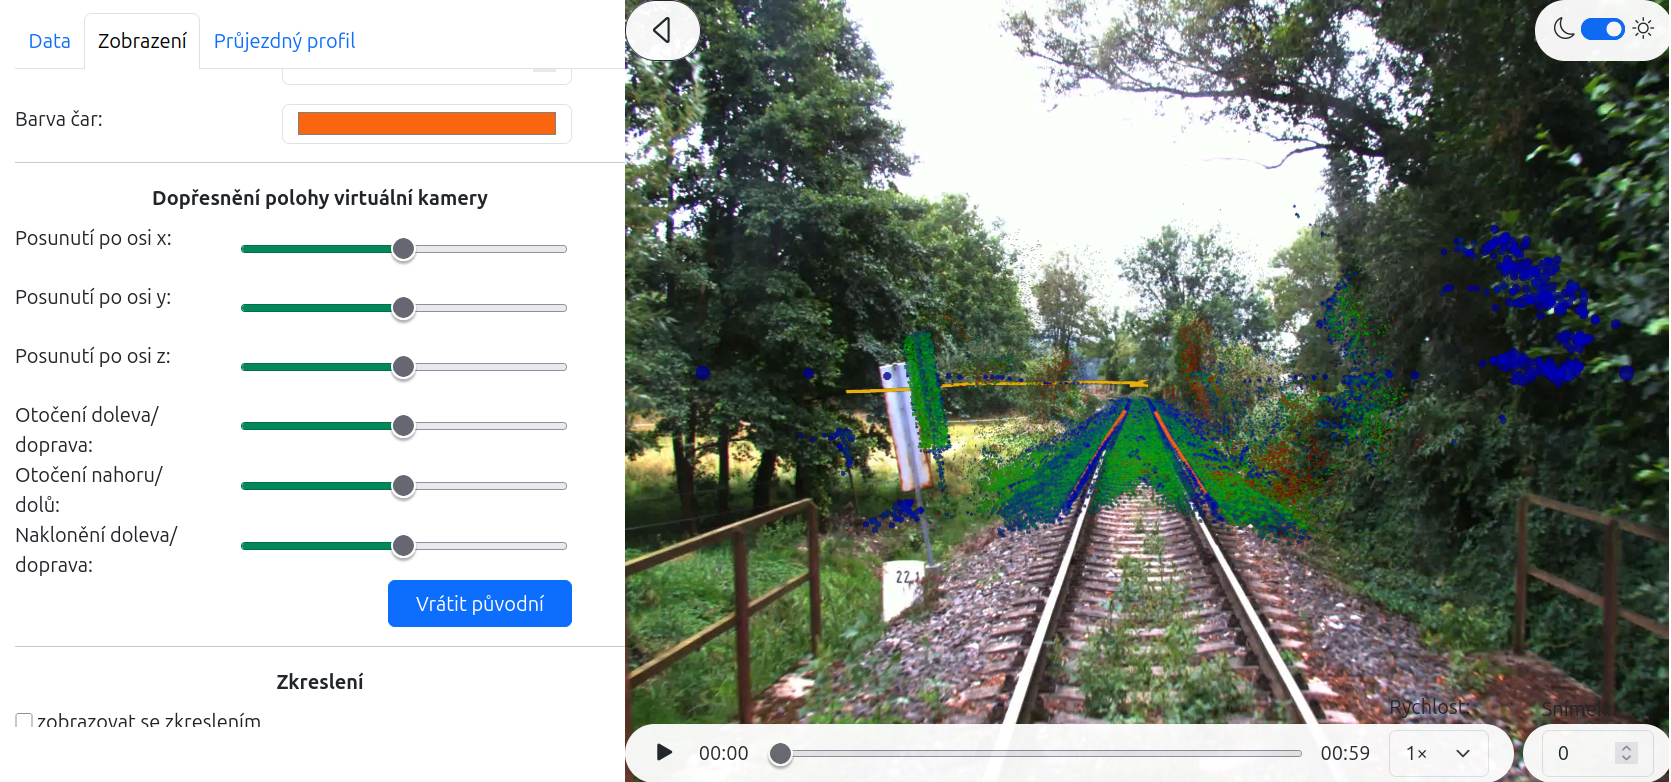
\includegraphics[width=0.9\linewidth]{text_prace/obrazky-figures/posuvniky1.png}
    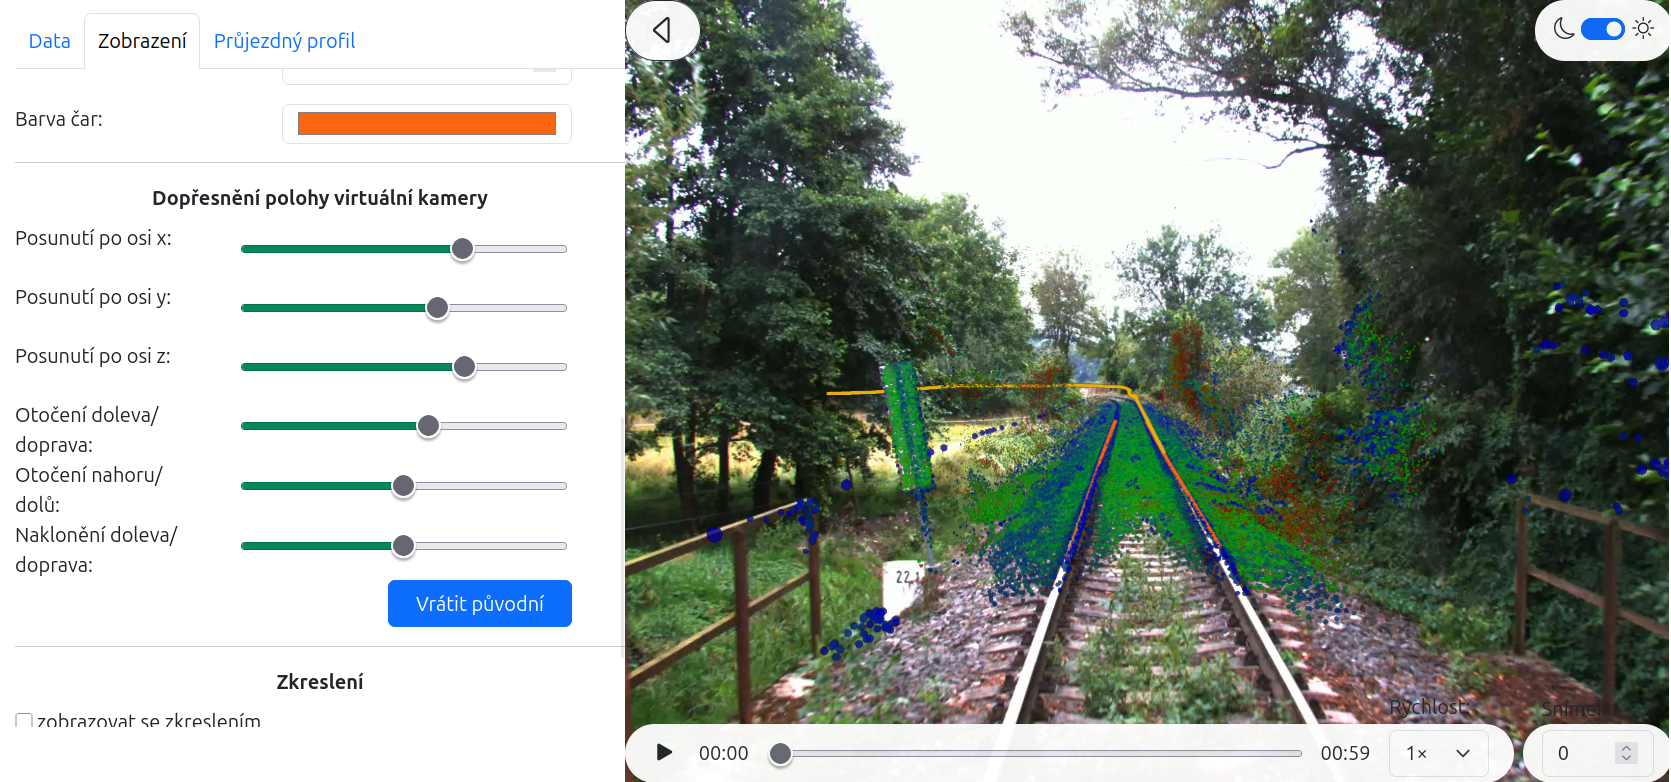
\includegraphics[width=0.9\linewidth]{text_prace/obrazky-figures/posuvniky2.png}
    \caption[Funkcionalita posuvníkov pre prispôsobenie polohy virtuálnej kamery.]{Funkcionalita posuvníkov pre prispôsobenie polohy virtuálnej kamery. Hore je zobrazenie bez prispôsobenia, dole s~prispôsobením.}
    \label{fig:posuvniky}
\end{figure}

\section{Optimalizácia vykresľovania mračna bodov}

V~priebehu implementácie bolo postupne vyskúšaných a porovnaných päť rôznych spôsobov vykresľovania mračna bodov:
\begin{enumerate}
    \item Použitie knižníc Pydeck a Dash Deck tak, ako je to vo vzorových príkladoch v~dokumentácii knižnice Dash Deck. Počítanie transformácií v~prístupových funkciách.
    \item Použitie iba knižnice Dash Deck, definícia vizualizácie pomocou slovníka. Počítanie transformácií v~prístupových funkciách.
    \item Použitie frameworku deck.gl priamo pomocou kódu v~jazyku JavaScript, riadenie animácie pomocou komponentu \texttt{Interval}\footnote{Funkcionalita komponentu \texttt{Interval} frameworku Dash spočíva v~tom, že periodicky spúšťa callback, pričom periódu určuje parameter \texttt{interval}.}. Počítanie transformácií v~prístupových funkciách. 
    \item Použitie frameworku deck.gl a riadenie animácie priamo pomocou kódu v~jazyku JavaScript. Počítanie transformácií v~prístupových funkciách.
    \item Použitie frameworku deck.gl a riadenie animácie priamo pomocou kódu v~jazyku JavaScript. Aplikovanie transformácií iba na kameru.
\end{enumerate}

Ukázalo sa, že každý z~týchto spôsobov je lepší ako tie uvedené pred ním, takže finálna implementácia, ako už bolo popísané v~predchádzajúcej kapitole, používa 5. spôsob.

Cieľom tejto sekcie je porovnať všetky tieto spôsoby a zdôvodniť, prečo je práve 5. spôsob najlepší.

Všetky v~tejto sekcii uvedené merania prebiehali na notebooku s~operačným systémom Ubuntu 24.04.1, procesorom Intel Core i5-9300H~×~8, grafickou kartou Intel UHD Graphics 630 (CFL GT2) a veľkosťou operačnej pamäte 16~GiB. Vykresľované mračno bodov obsahovalo 201~880 bodov a spolu s~jeho zobrazovaním sa prehrávalo aj video.

\subsubsection{1. spôsob}

Prvý spôsob je výrazne neefektívny. Pri implementácii týmto spôsobom jedno vykreslenie mračna bodov zaberá zhruba 3 sekundy, čo je spôsobené transformáciami medzi rôznymi formátmi, ako to bolo popísané v~sekcii \ref{sec:deck_gl}.

\subsubsection{2. spôsob}

 Meranie výkonnosti je uvedené v~tabuľke \ref{tab:meranie_sposob_2} a predstavuje najlepší výsledok, aký bolo možné dosiahnuť iba pomocou kódu v~jazyku Python, bez použitia jazyka JavaScript.

\begin{table}[h]
    \centering
    \begin{tabular}{>{\centering\arraybackslash}m{10em}|>{\centering\arraybackslash}m{13em}|>{\centering\arraybackslash}m{12em}}
        {\RaggedRight Nastavenie parametra \texttt{interval} [ms]} &  {\RaggedRight Čas, za ktorý prebehla celá animácia (100 snímok) [s]} & {\RaggedRight Priemerný čas vykreslenia jednej snímky [ms]} \\ \hline
        1000 & 101 & 1010 \\
        800 & 80 & 800 \\
        750 & 76 & 760 \\
        700 & 72 & 720 \\
        650 & 71 & 710 \\
        600 & 70 & 700 \\
    \end{tabular}
    \caption{Výkonnosť animácie pohybu vlaku pri použití 2. spôsobu vykresľovania mračna bodov (použitie knižnice Dash Deck). Z~nameraných údajov vyplýva, že minimálny čas potrebný na vykreslenie jednej snímky je asi 750~ms, čo znamená, že rýchlosť nedosahuje ani 2 snímky za sekundu.}
    \label{tab:meranie_sposob_2}
\end{table}

Podľa nameraných údajov tento spôsob predstavuje významné zlepšenie oproti prvému spôsobu, ani on však nie je dosť výkonný na to, aby umožnil hladký beh animácie pohybu vlaku. Príčina neefektivity je v~spôsobe implementácie knižnice Dash Deck, ktorá zrejme, podobne ako Pydeck, nie je stavaná na to, aby sa vo vizualizácii robili časté zmeny.

\subsubsection{3. spôsob}

Ide vlastne o~medzistupeň medzi 2. a 4. spôsobom, kedy je už vizualizácia riadená priamo pomocou kódu v~jazyku JavaScript, ale riadenie animácie zostáva v~réžii frameworku Dash.

Meranie výkonnosti je v~tabuľke \ref{tab:meranie_sposob_3} a profiling na obrázku \ref{fig:profiling_interval}.

\begin{table}[h]
    \centering
    \begin{tabular}{>{\centering\arraybackslash}m{10em}|>{\centering\arraybackslash}m{13em}|>{\centering\arraybackslash}m{12em}}
         Nastavenie parametra \texttt{interval} [ms] &  Čas, za ktorý prebehla celá animácia (500 snímok) [s] & Priemerný čas vykreslenia jednej snímky [ms] \\ \hline
        250 & 126 & 252 \\
        200 & 101 & 202 \\
        150 & 76 & 152 \\
        125 & 68 & 136 \\
        100 & 63 & 126 \\
         75 & 62 & 124 \\
    \end{tabular}
    \caption{Výkonnosť animácie pohybu vlaku pri použití 3. spôsobu vykresľovania mračna bodov (riadenie vizualizácie v~JavaScripte, riadenie animácie v~Pythone). Použité technológie: Python, Dash, Javascript, deck.gl. Z~nameraných údajov vyplýva, že minimálny čas potrebný na vykreslenie jednej snímky je asi 150~ms, čo zodpovedá rýchlosti asi 6 snímok za sekundu.}
    \label{tab:meranie_sposob_3}
\end{table}

Aj tento spôsob priniesol zlepšenie oproti tomu predchádzajúcemu, ale stále nie je dostatočný na hladký beh animácie. Riadenie animácie pomocou komponentu \texttt{Interval} frameworku Dash je totiž pomerne ťažkopádne, pretože funguje na základe komunikácie medzi klientom a serverom a tým animáciu spomaľuje. Preto bolo vhodné nahradiť ho riadením animácie v~jazyku JavaScript výhradne na strane klienta.

\begin{figure}
    \centering
    \begin{subfigure}[b]{1\textwidth}
        \centering
        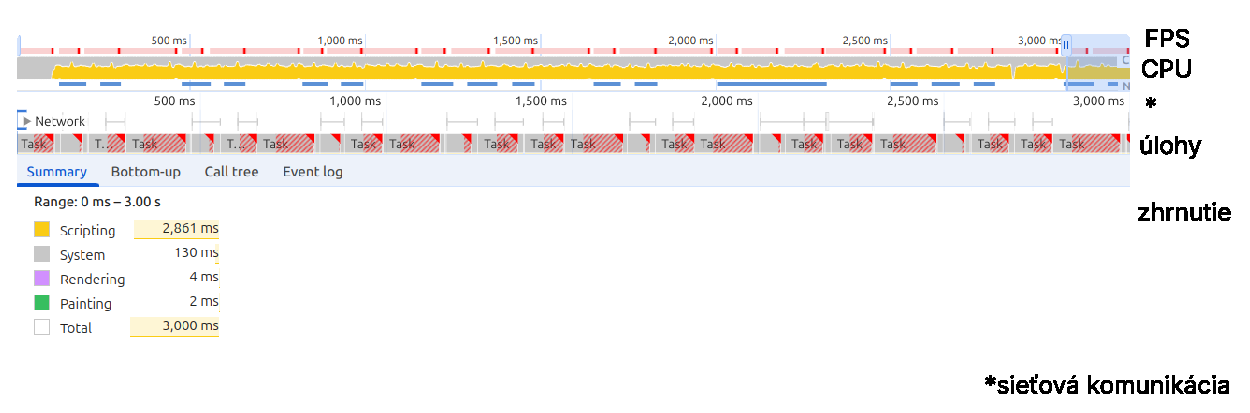
\includegraphics[width=1\linewidth]{text_prace/obrazky-figures/profiling_interval.pdf}
        \caption{3. spôsob, riadenie pomocou komponentu \texttt{Interval} a počítanie transformácií v~prístupových funkciách.}
        \label{fig:profiling_interval}
    \end{subfigure}
    \hfill
    \begin{subfigure}[b]{1\textwidth}
        \centering
        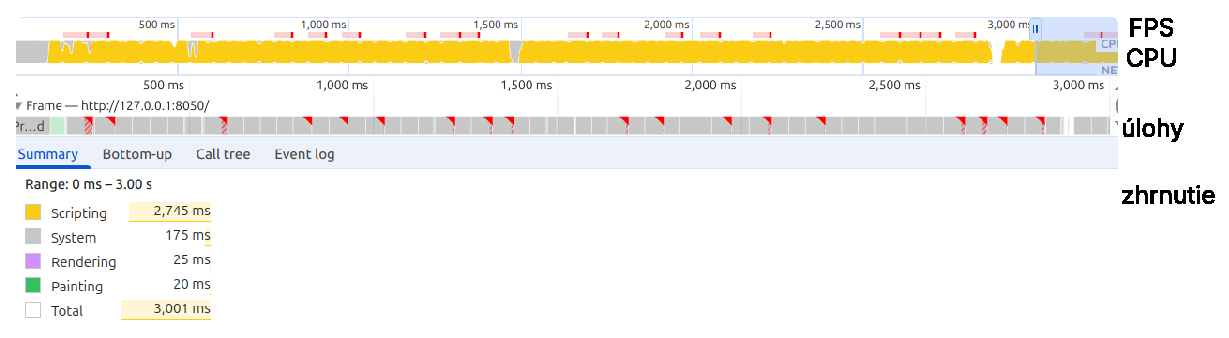
\includegraphics[width=1\linewidth]{text_prace/obrazky-figures/profiling1.pdf}
        \caption{4. spôsob, riadenie pomocou kódu v~jazyku JavaScript a počítanie transformácií v~prístupových funkciách.}
        \label{fig:profiling1}
    \end{subfigure}
    \hfill
    \begin{subfigure}[b]{1\textwidth}
        \centering
        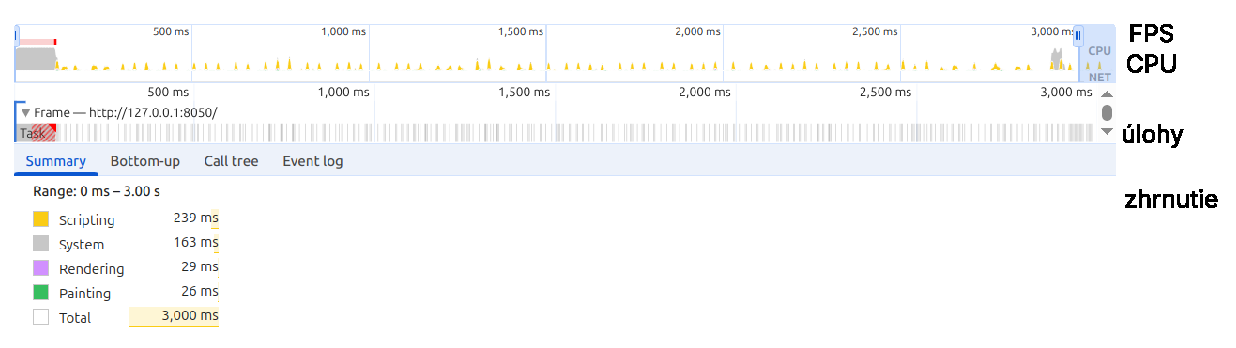
\includegraphics[width=1\linewidth]{text_prace/obrazky-figures/profiling2.pdf}
        \caption{5. spôsob, riadenie pomocou kódu v~jazyku JavaScript a aplikovanie transformácií iba na kameru.}
        \label{fig:profiling2}
    \end{subfigure}
    \caption[Profiling animácie pohybu vlaku pri použití rôznych spôsobov vykresľovania mračna bodov.]{Profiling animácie pohybu vlaku pri použití rôznych spôsobov vykresľovania mračna bodov. Každý graf zachytáva tri sekundy behu animácie. Profiling prebiehal v~prehliadači Google Chrome 133.0.6943.126 s~rozmermi okna 1480×832 pixelov. Bol použitý profiler vstavaný v~tomto prehliadači.}
    \label{fig:profiling}
\end{figure}

\subsubsection{4. spôsob}

Zmenu oproti predchádzajúcemu spôsobu je iba iný typ riadenia animácie, ktorý je použitý aj vo finálnej verzii implementácie a detailne popísaný v~sekcii \ref{sec:implementacia_animacie}.

Profiling tohto spôsobu je na obrázku \ref{fig:profiling1}. Pri porovnaní s~profilingom predchádzajúceho spôsobu sa ukázalo, že hoci sa zvýšilo zaťaženie procesora, výrazne sa znížil čas potrebný na vykreslenie jednej snímky animácie, čo umožnilo vykreslenie väčšieho počtu snímok za sekundu (v~grafoch sekcia \emph{úlohy}).

U~tohto spôsobu už animácia vyzerala plynulo, ale výkon aplikácie stále nebol vyhovujúci, pretože animácia výrazne zaťažovala procesor a hodnota snímkovej frekvencie stále miestami dosahovala príliš nízke hodnoty (v~grafoch červené čiary v~sekcii \emph{FPS}).

\subsubsection{5. spôsob}

V~sekcii \ref{sec:nastavenie_polohy_kamery} boli popísané dva rôzne spôsoby nastavenia polohy kamery vo frameworku deck.gl. U~vyššie popísaných spôsobov vykresľovania mračna bodov bol použitý ten prvý, teda výpočet transformácií pomocou prístupových funkcií, pretože je implementačne jednoduchší. Tento posledný, 5. spôsob sa od 4. spôsobu líši iba tým, že nepoužíva prístupové funkcie a transformácie aplikuje iba na kameru, nie na body. 

Profiling tohto spôsobu vykresľovania mračna bodov je na obrázku \ref{fig:profiling2}. Z~nameraných údajov vyplýva, že táto optimalizácia veľmi výrazne znížila zaťaženie procesora. Zatiaľ čo pri 4. spôsobe sa počas trojsekudového intervalu vykonával javascriptový kód 2,745 sekúnd, pri tomto spôsobe to bolo iba 239 milisekúnd, čo predstavuje viac než desaťnásobné zníženie.

Dôležitou metrikou pri posudzovaní výkonnosti animácií je snímková frekvencia meraná v~FPS (\emph{frames per second}, počet vykreslených snímok za sekundu). V~ideálnom prípade by sa snímková frekvencia mala blížiť 60~FPS, pretože vtedy sa animácia ľudskému oku zdá hladká \cite{chrome_profiling}.

Podľa vstavaného ukazovateľa snímkovej frekvencie v~prehliadači Google Chrome dosahovala skúmaná animácia pri 4. spôsobe vykresľovania mračna bodov zhruba 28 až 34~FPS, zatiaľ čo pri 5. spôsobe 51 až 55~FPS. Aj v~tomto ohľade teda nastalo významné zlepšenie.

\section{Výkonnosť}

Na výkonnosť aplikácie má najväčší vplyv mračno bodov. Táto sekcia obsahuje merania, aký výkon dosahuje aplikácia pri prehrávaní animácie s~mračnami bodov rôznych veľkostí. Merania prebiehali s~rovnakými technológiami ako v~predchádzajúcej kapitoly, na meranie záťaže procesora a využitia pamäte bol použitý nástroj Chrome Task Manager.

Výsledky merania výkonnosti animácie s~mračnom bodov typu postprocess sú v~tabuľkách \ref{tab:vykonnost_postprocess} a \ref{tab:vykonnost_postprocess_so_skreslenim}. 

U~animácie bez skreslenia bola snímková frekvencia (FPS) dobrá až do menších jednotiek miliónov bodov, potom začala klesať. Deväť miliónov bodov už aplikácia nezvládla vôbec, pretože veľkosť dát spôsobila chybu vo frameworku Dash. Aby bola aplikácia schopná zobrazovať mračná bodov obsahujúce viac než osem miliónov bodov, musela by prejsť úpravou a deliť dáta na viacero častí. 

Naopak u~animácie so skreslením bola snímková frekvencia veľmi zlá aj pri menšom počte bodov, z~čoho vyplýva, že je implementovaná neefektívne a že režim so zobrazením skreslenia nie je vhodný na prehrávanie animácie.

Okrem snímkovej frekvencie bolo merané aj zaťaženie procesora. 100~\% hodnoty CPU v~tabuľke zodpovedá jednému plne bežiacemu jadru procesora. Táto hodnota je veľmi variabilná, ale u~animácie s~výpočtom skreslenia je mierne vyššia, čo je očakávané, pretože výpočet skreslenia prebieha na procesore.

\begin{table}[t]
    \centering
    \begin{tabular}{r||c|c}
        Počet bodov & FPS & CPU (\%) \\ \hline
        $200\times10^3$ & 51-54 & 70-210 \\
        $500\times10^3$ & 48-51 & 90-160 \\
        $1\times10^6$ & 47-50 & 60-190 \\
        $2\times10^6$ & 45-50 & 70-170 \\
        $5\times10^6$ & 30-42 & 70-250 \\
        $8\times10^6$ & 21-24 & 70-190 \\
        $9\times10^6$ & -- & -- \\
    \end{tabular}
    \caption{Výkonnosť vykresľovania mračna bodov typu postprocess \emph{bez výpočtu skreslenia} v~závislosti od počtu bodov, so zmenou polohy kamery desaťkrát za sekundu. V~dodaných dátach jeden milión bodov zodpovedal približne štyridsiatim sekundám záznamu z~lidaru.}
    \label{tab:vykonnost_postprocess}
\end{table}

\begin{table}[t]
    \centering
    \begin{tabular}{r||c|c}
        Počet bodov & FPS & CPU (\%) \\ \hline
        $50\times10^3$ & 4-5 & 140-200 \\
        $100\times10^3$ & 3-4 & 130-240 \\
        $200\times10^3$ & 2-4 & 150-180 \\
        $500\times10^3$ & 1-3 & 130-180 \\
        $1\times10^6$ & 2-4 & 70-230 \\
        $2\times10^6$ & 1-3 & 70-230 \\
    \end{tabular}
    \caption{Výkonnosť vykresľovania mračna bodov typu postprocess \emph{s~výpočtom skreslenia} v~závislosti od počtu bodov, so zmenou polohy kamery desaťkrát za sekundu.}
    \label{tab:vykonnost_postprocess_so_skreslenim}
\end{table}

Ďalej prebehlo meranie výkonnosti animácie s~mračnom bodov typu real-time, ktorého výsledky sú v~tabuľke \ref{tab:vykonnost_postprocess}.

Z~meraní vyplýva, že snímková frekvencia je veľmi dobrá a aplikácii nerobí problém ani zvýšenie počtu bodov či frekvencie striedania častí. Zaťaženie procesora je dokonca menšie a~menej variabilné než u~mračna bodov typu postprocess.

Celkovým záverom z~tohto testovania je, že animácia má dobrú výkonnosť, ale iba bez výpočtu skreslenia. U~mračna bodov typu postprocess sa výkon začína zhoršovať u~nižších jednotiek miliónov bodov a maximálny počet bodov, ktorý aplikácia zvládne vykresliť, je osem miliónov.

\begin{table}[t]
    \centering
    \begin{tabular}{c|c||c|c}
        Počet bodov v~1 časti & Frekvencia snímania ($s^{-1}$) & FPS & CPU (\%) \\ \hline
        { }$1\times10^3$ & 10 & 50-55 & 70-90 \\
        { }$2\times10^3$ & 10 & 50-54 & 70-90 \\
        { }$5\times10^3$ & 10 & 49-53 & 70-120 \\
        $10\times10^3$ & 10 & 49-54 & 70-110 \\ \hline
        { }$1\times10^3$ & 25 & 48-53 & 70-90 \\
        { }$2\times10^3$ & 25 & 48-54 & 80-110 \\
        { }$5\times10^3$ & 25 & 48-53 & 80-110 \\
        $10\times10^3$ & 25 & 47-52 & 90-120 \\
    \end{tabular}
    \caption{Výkonnosť vykresľovania mračna bodov typu real-time \emph{bez výpočtu skreslenia} v~závislosti od počtu bodov v~jednej časti mračna bodov a frekvencie snímania týchto častí lidarom. Frekvencia zmien polohy kamery bola pri testovaní totožná s~frekvenciou snímania. V~dodaných dátach bolo v~jednej časti priemerne 2615 bodov a frekvencia snímania bola približne 10 častí za sekundu.}
    \label{tab:vykonnost_realtime}
\end{table}

\section{Vyhodnotenie používateľskej prívetivosti}

Zisťovanie použítaveľskej prívetivosti aplikácie prebiehalo v~dvoch etapách.

V~prvej etape bolo malému počtu účastníkov dané za úlohu iba oboznámiť sa s~aplikáciou a zistiť, aká je jej funkcionalita. Účastníci boli pritom osobne sledovaní a cieľom bolo zistiť, či je aplikácia dostatočne intuitívna, teda či je na prvý pohľad zrejmá funkcionalita každého prvku.

\pagebreak

Závery boli nasledujúce:
\begin{itemize}
    \item Prvky v~používateľskom rozhraní nie sú dobre usporiadané, je potrebné ich preskupiť.
    \item K~niektorým prvkom je potrebné pridať popis.
    \item Pre používateľov by bolo intuitívnejšie meniť farebnú škálu klikaním do grafu než použitím číselných vstupov pod ním.
\end{itemize}

Prvé dva body boli vyriešené, tretí nie, pretože je implementačne náročnejší.

Druhá etapa testovania mala jedenásť dobrovoľných účastníkov a prebiehala pomocou dotazníka. Používatelia dostali štyri úlohy, ktoré sa mali pokúsiť pomocou aplikácie vyriešiť, a potom vyplniť~dotazník. Úlohy boli zámerne jednoduché, pretože ich cieľom bolo iba to, aby si účastníci vyskúšali prácu s~aplikáciou.

Nedokonalosťou testovania bola skutočnosť, že používatelia, s~ktorými bola aplikácia testovaná, neboli cieľovými používateľmi, teda ľuďmi, ktorí pracujú s~dátami z~mobilných mapovacích systémov, ale na túto skutočnosť bol braný ohľad a veci, ktoré by im mohli byť nejasné, boli vysvetlené.

Prvou časťou dotazníka bolo meranie použiteľnosti metódou \emph{System Usability Scale} (SUS). Táto metóda je rýchla a jednoduchá a zakladá sa na desiatich tvrdeniach, na ktoré účastník testovania vyberá odpoveď v~rozmedzí \uv{rozhodne nesúhlasím -- skôr nesúhlasím -- neviem -- skôr súhlasím -- rozhodne súhlasím}. Tvrdenia sú usporiadané tak, že sa striedajú tie, na ktoré majú účastníci tendenciu odpovedať skôr kladne a tie, na ktoré majú tendenciu odpovedať skôr záporne, čo ich núti neodpovedať mechanicky a skutočne sa nad každým tvrdením zamyslieť. Odpovede sa následne obodujú a spočíta sa skóre od 0 do 100 \cite{brooke_sus}.

Podľa článku J. Saura na stránke spoločnosti MeasuringU sa SUS stalo široko používanou metódou a systémy dosahujú priemerné SUS skóre 68 \cite{sauro_sus}. Testovaná aplikácia získala skóre 78,2, čo podľa grafu publikovaného v~tomto článku zodpovedá približne percentilu 82, a je to teda nadpriemerný výsledok.

V~druhej časti dotazníka mali účastníci testovania priestor na napísanie postrehov a návrhov na vylepšenia. Podali nasledovné návrhy:
\begin{enumerate}
    \item panel nástrojov by mal byť implicitne otvorený akebo lepšie zviditeľnený ($3\times$),
    \item aplikácia by mala obsahovať nápovedy ($2\times$),
    \item pridanie ovládania pomocou klávesnice,
    \item zobrazenie \uv{progress baru} pri načítaní,
    \item pridanie legendy ku grafu,
    \item skrytie nastavení farieb a hrúbok čiar, pretože to nie je dôležitá vlastnosť,
    \item pridanie prednastavených módov.
\end{enumerate}

Jeden účastník upozornil na chybu, ktorú sa podarilo reprodukovať v~prehliadači Google Chrome a následne opraviť.

\chapter{Záver}

Cieľom tejto práce bolo vytvoriť systém pre vizualizáciu dát z~mobilného mapovacieho systému. Tento cieľ bol splnený.

Návrh systému zahŕňal návrh funkcionality aj používateľského rozhrania. Systém bol implementovaný ako webová aplikácia v~programovacom jazyku Python s~využitím frameworku Dash\footnote{Zdrojové kódy vytvorenej aplikácie sú voľne dostupné na stránke \url{https://github.com/xmiska03/RailwayDataVisualization}.}. Bolo preskúmaných niekoľko rozdielnych spôsobov implementácie vykresľovania mračna bodov pomocou rôznych technológií, z~ktorých bol vybraný ten najlepší, a~to vloženie skriptu v~jazyku JavaScript, ktorý beží na strane klienta a využíva hardvérovo akcelerovaný framework deck.gl. Bola vyhodnotená výkonnosť a používateľská prívetivosť aplikácie.

Pre zjednodušenie nahrávania dát do aplikácie bol navrhnutý špeciálny projektový súbor, ktorý je možné využiť, ak má používateľ prístup k~serveru, na ktorom aplikácia beží.

Výsledná aplikácia má dobrú výkonnosť s~výnimkou výpočtu skreslenia. U~mračna bodov typu postprocess sa výkon začína zhoršovať u~nižších jednotiek miliónov bodov a aplikácia zvládne mračná bodov do maximálnej veľkosti 8 miliónov bodov. Aplikácia spĺňa v~dostatočnej miere všetky vlastnosti popísané v~návrhu.

Aplikácia bola testovaná s~použitím metódy \emph{System Usability Scale}. Testovanie zahŕňalo jedenásť účastníkov, ktorí dali aplikácii nadpriemerné hodnotenie a navyše poskytli aj užitočné podnety na jej ďalšie zlepšenie.

V~práci by bolo možné pokračovať pridaním možnosti zobrazovať dáta streamované v~reálnom čase. Existuje ešte mnoho možných zlepšení funkcionality aj používateľského rozhrania, napríklad rozšírenie možností nahrávania dát, umožnenie nastavenia farebnej škály klikaním do grafu, filtrácia mračna bodov a optimalizácia výpočtu skreslenia. Hodilo by sa pridať validáciu nahrávaných dát a upozorniť používateľa chybovou hláškou, ak nahrá dáta v~nesprávnom formáte.

V~dlhodobejšom horizonte by bolo možné prácu rozšíriť okrem vizualizácie aj o~niektoré možnosti spracovania mračna bodov, napríklad kolorizáciu podľa videa.

%===============================================================================

% Pro kompilaci po částech (viz projekt.tex) nutno odkomentovat
%\end{document}


  \fi
  
  % Kompilace po částech (viz výše, nutno odkomentovat a zakomentovat input výše)
  % Compilation piecewise (see above, it is necessary to uncomment it and comment out input above)
  %\subfile{chapters/projekt-01-uvod-introduction}
  % ...
  %\subfile{chapters/projekt-05-zaver-conclusion}

  % Pouzita literatura / Bibliography
  % ----------------------------------------------
\ifslovak
  \makeatletter
  \def\@openbib@code{\addcontentsline{toc}{chapter}{Literatúra}}
  \makeatother
  \bibliographystyle{bib-styles/Pysny/skplain}
\else
  \ifczech
    \makeatletter
    \def\@openbib@code{\addcontentsline{toc}{chapter}{Literatura}}
    \makeatother
    \bibliographystyle{bib-styles/Pysny/czplain}
  \else 
    \makeatletter
    \def\@openbib@code{\addcontentsline{toc}{chapter}{Bibliography}}
    \makeatother
    \bibliographystyle{bib-styles/Pysny/enplain}
  %  \bibliographystyle{alpha}
  \fi
\fi
  \begin{flushleft}
  \bibliography{xmiska03-Zobrazeni_dat_z_zeleznicniho_MMS-20-literatura-bibliography}
  \end{flushleft}

  % vynechani stranky v oboustrannem rezimu
  % Skip the page in the two-sided mode
  \iftwoside
    \cleardoublepage
  \fi

  % Prilohy / Appendices
  % ---------------------------------------------
  \appendix
\ifczech
  \renewcommand{\appendixpagename}{Přílohy}
  \renewcommand{\appendixtocname}{Přílohy}
  \renewcommand{\appendixname}{Příloha}
\fi
\ifslovak
  \renewcommand{\appendixpagename}{Prílohy}
  \renewcommand{\appendixtocname}{Prílohy}
  \renewcommand{\appendixname}{Príloha}
\fi
%  \appendixpage

% vynechani stranky v oboustrannem rezimu
% Skip the page in the two-sided mode
%\iftwoside
%  \cleardoublepage
%\fi
  
\ifslovak
%  \section*{Zoznam príloh}
%  \addcontentsline{toc}{section}{Zoznam príloh}
\else
  \ifczech
%    \section*{Seznam příloh}
%    \addcontentsline{toc}{section}{Seznam příloh}
  \else
%    \section*{List of Appendices}
%    \addcontentsline{toc}{section}{List of Appendices}
  \fi
\fi
  \startcontents[chapters]
  \setlength{\parskip}{0pt} 
  % seznam příloh / list of appendices
  % \printcontents[chapters]{l}{0}{\setcounter{tocdepth}{2}}
  
  \ifODSAZ
    \setlength{\parskip}{0.5\bigskipamount}
  \else
    \setlength{\parskip}{0pt}
  \fi
  
  % vynechani stranky v oboustrannem rezimu
  \iftwoside
    \cleardoublepage
  \fi
  
  % Přílohy / Appendices
  \ifenglish
    \input{xmiska03-Zobrazeni_dat_z_zeleznicniho_MMS-30-prilohy-appendices-en}
  \else
    % Tento soubor nahraďte vlastním souborem s přílohami (nadpisy níže jsou pouze pro příklad)

% Pro kompilaci po částech (viz projekt.tex), nutno odkomentovat a upravit
%\documentclass[../projekt.tex]{subfiles}
%\begin{document}

% Umístění obsahu paměťového média do příloh je vhodné konzultovat s vedoucím
%\chapter{Obsah přiloženého paměťového média}

%\chapter{Manuál}

\chapter{Projektový súbor}
\label{ch:project_file}

Pre nahrávanie dát do implementovanej aplikácie bol navrhnutý jednoduchý jednoúrovňový projektový súbor vo formáte TOML, ktorého štruktúra je popísaná tabuľkou \ref{tab:projektovy_subor}.

\begin{landscape}
\begin{longtable}{>{}p{20em}|>{}p{8em}|>{}p{28em}}
    \caption{Štruktúra projektového súboru.}
    \label{tab:projektovy_subor} \\
    
    Názov premennej & Dátový typ & Popis \\ \hline \hline
    \texttt{project\_path} & reťazec & Absolútna cesta k~priečinku s~projektom. Všetky ostatné cesty sú relatívne vzhľadom k~tomuto priečinku. \\ \hline
    \texttt{postprocess\_pcd\_path} & reťazec & Relatívna cesta k~súboru s~mračnom bodov typu postprocess vo formáte \texttt{pcd}. \\ \hline
    \texttt{realtime\_pcd\_path} & reťazec & Relatívna cesta k~priečinku so súbormi s~mračnom bodov typu real-time vo formáte \texttt{pcd}. \\ \hline
    \texttt{realtime\_pcd\_filename\_prefix} & reťazec & Prefix názvov týchto súborov\footnote{Jednotlivé súbory musia byť pomenované \texttt{[prefix]\_0.pcd}, \texttt{[prefix]\_1.pcd}, atď.}. \\ \hline
    \texttt{realtime\_pcd\_files\_cnt} & prirodzené číslo & Počet týchto súborov. \\ \hline
    \texttt{realtime\_pcd\_timestamps\_path} & reťazec & Relatívna cesta k~súboru s~časovými razítkami mračna bodov typu real-time vo formáte \texttt{txt}\footnote{Každý riadok súboru musí byť vo formáte \texttt{[cislo\_riadku] [casove\_razitko]}.}. \\ \hline
    \texttt{video\_path} & reťazec & Relatívna cesta k~súboru s~videom vo formáte \texttt{mp4}, s~kódovaním H.264. \\ \hline
    \texttt{vector\_data\_path} & reťazec & Relatívna cesta k~priečinku so súbormi s~vektorovými dátami vo formáte \texttt{csv}. \\ \hline
    \texttt{translations\_path} & reťazec & Relatívna cesta k~súboru s~transláciami kamery vo formáte \texttt{csv}. \\ \hline
    \texttt{rotations\_path} & reťazec & Relatívna cesta k~súboru s~rotáciami kamery vo formáte \texttt{csv}. \\ \hline
    \texttt{timestamps\_path} & reťazec & Relatívna cesta k~súboru s~časovými razítkami polôh kamery vo formáte \texttt{csv}. \\ \hline
    \texttt{profile\_translations\_path} & reťazec & Relatívna cesta k~priečinku so súbormi s~transláciami prejazdného profilu vo formáte \texttt{csv}\footnote{Každý riadok súboru musí byť vo formáte \texttt{[x] [y] [z]}. Jednotlivé súbory musia byť pomenované \texttt{[prefix]\_25.csv}, \texttt{[prefix]\_50.csv}, \texttt{[prefix]\_75.csv}, \texttt{[prefix]\_100.csv}.}. \\ \hline
    \texttt{profile\_translations\_filename\_prefix} & reťazec & Prefix názvov týchto súborov. \\ \hline
    \texttt{profile\_rotations\_path} & reťazec & Relatívna cesta k~priečinku so súbormi s~rotáciami prejazdného profilu vo formáte \texttt{csv}\footnote{Každý riadok súboru musí byť vo formáte \texttt{[yaw] [pitch] [roll]}.}. \\ \hline
    \texttt{profile\_rotations\_filename\_prefix} & reťazec & Prefix názvov týchto súborov. \\ \hline
    \texttt{calibration\_matrix} & pole 9 čísel & Kalibračná matica. \\ \hline
    \texttt{far\_plane} & prirodzené číslo & Vzdialenosť zadnej orezávacej roviny v metroch. \\ \hline
    \texttt{distortion\_parameters} & pole 5 čísel & Parametre skreslenia kamery.
\end{longtable}
\end{landscape}

%\chapter{Plakát}

% Pro kompilaci po částech (viz projekt.tex) nutno odkomentovat
%\end{document}

  \fi
  
  % Kompilace po částech (viz výše, nutno odkomentovat)
  % Compilation piecewise (see above, it is necessary to uncomment it)
  %\subfile{xmiska03-Zobrazeni_dat_z_zeleznicniho_MMS-30-prilohy-appendices}
  
\end{document}

